\documentclass[
	%parspace, % Add vertical space between paragraphs
	%noindent, % No indentation of first lines in each paragraph
	%nohyp, % No hypenation of words
	%twoside, % Double sided format
	%draft, % Quicker draft compilation without rendering images
	%final, % Set final to hide todos
]{classes/TDK_en}[2023/04/10]


\title{Scalable Distributed Reinforcement Learning in Multi-Agent Environments}
\date{2024}

% Author(s)' metadata
\author{Gergely Magyar}
\degree{Computer Science MSc}
\period{2. grade}
\coauthor{Tamás Takács}
\codegree{Computer Science MSc}
\coperiod{2. grade}
\neptuncode{DEXFD3}
\coneptuncode{CJRNIE}

% Superivsor(s)' metadata
\supervisor{László Gulyás}
\affiliation{Associate Professor\protect\\Department of Artificial Intelligence\protect\\Faculty of Informatics}

% University's metadata
\university{Eötvös Loránd University}
\faculty{Faculty of Informatics}
\department{Dept. of Artificial Intelligence}
\city{Budapest}
\logo{elte_cimer_szines}

% Add bibliography file
\addbibresource{bibliography/TDK_en.bib}

% number subsubsections
\setcounter{secnumdepth}{3}

% The document
\begin{document}

% Set document language
%\documentlang{hungarian}
\documentlang{english}

% List of todos (not in the final document)
%\listoftodos[\todolabel]
%\cleardoublepage

% Cover and title page (mandatory)
%\makecover
\cleardoublepage
\maketitle

% Table of contents (mandatory)
\hypersetup{linkcolor=black}
\tableofcontents
\hypersetup{linkcolor=deepblue}
\cleardoublepage

\clearpage
\newgeometry{left=3.5cm, right=3.5cm, top=2.5cm, bottom=2.5cm}
\chapter*{\centering Abstract}
\addcontentsline{toc}{chapter}{Abstract}
\label{ch:abst}

\noindent Novel reinforcement learning algorithms often face scalability and compatibility issues in multi-agent environments, as they are primarily benchmarked and optimized for single-agent settings. The lack of a standardized method for adapting these algorithms to multi-agent contexts restricts their broader applicability. In multi-agent environments where the number of controllable entities can rapidly change over a short timeframe and can scale up to massive numbers, making the utilization of both monolithic and distributed architectures challenging to orchestrate. This complexity arises from the difficulty of credit assignment, extensive memory usage, and increased computational time, leading to slow, destabilized training and suboptimal resource utilization. In our work, we explore various methods to help alleviate such inefficiencies. We worked in a massively dynamic multi-agent, open-source environment featured in a Kaggle competition called Lux AI. For this setting, we study a novel implementation of a monolithic agent control method from the literature and demonstrate that a single-brain global outlook is insufficient for managing populous environments. We propose a \textbdd{hybrid architecture}, combining the strengths of monolithic and distributed approaches, which led to a \textbdd{30-times reduction in model size} compared to the best-performing reinforcement learning submission to the competition while still being able to learn basic skills needed in the environment \textbdd{24 times faster} in terms of training time and with \textbdd{600-times fewer examples} of training data. We also introduce a technique called \textbdd{trajectory separation} to massively speed up convergence, yielding a \textbdd{3-times speed increase in training speed} over our initial trials. Using our approach, we achieved a \textbdd{5-times reduction in training epochs} needed to reach our designated milestone compared to the baseline model provided by the competition organizers while producing comparable results with \textbdd{2-times less trainable parameters}.

\restoregeometry



\cleardoublepage

% Main content
\chapter{Introduction}
\label{ch:intro}

\vspace{-2.5em}

\noindent In recent years, Multi-agent Reinforcement Learning (MARL) has experienced a significant surge in research activity, driven by the ongoing AI advancements and substantial funding dedicated to this field (\cite{gilbert2023reward}). The global market for MARL was valued at $2.8$ billion in 2022, with projections indicating a robust compound annual growth rate (CAGR) of $41.5\%$ from 2023 to 2032. By 2032, it is anticipated to soar to a remarkable $\$88.7$ billion (\cite{reinforcementLearningMarket2023}). Advancements in academic research indicate an upcoming trend where both implicit and explicit Reinforcement Learning (RL) systems will display heightened efficacy. These systems are poised to find more general applications in user-facing domains, delivering more significant impacts (\cite{kirk2023personalisation}).

\bigskip

\noindent A significant portion of contemporary research dedicates efforts to exploring emergent intelligence within cooperative environments, serving as a bridge between current research and the pursuit of Artificial General Intelligence (AGI) (\textcolor{deepblue}{\cite{lowe2020multiagent}; \cite{foerster2018learning}}). These studies center on environments that abstract real-world scenarios, characterized by interacting agents, diverse interests, varied goals, and the sharing of resources. Such environments inherently possess dynamism, displaying both evolving environmental conditions and fuzzy goal dynamics. Research has also demonstrated that competitive environments often foster heightened cooperation among agents (\textcolor{deepblue}{\cite{openai2019dota}; \cite{baker2020emergent}}). By utilizing multiple trajectories, the learning agent can gain experience from a wider array of interactions, with more players enhancing the diversity of trajectories encountered. In such settings, agent's objectives shift towards overcoming opposing teams, leading to continual refinement of policies until they surpass those of the opposing team. Competition inherently promotes dynamic interactions, devoid of a stable \textbdd{Nash equilibrium}, thereby promoting ongoing adaptation and the perpetual search to outwit the opposing team. Nash Equilibrium is a set of strategies, one for each player, such that no player has an incentive to deviate unilaterally from their strategy, given the strategies of the other players (\cite{doi:10.1073/pnas.36.1.48}; \cite{Nash1951}). In a zero-sum game, the gain of one participant is exactly offset by the losses of other participants, as the total amount of resources available is fixed. Therefore, any resource gained by one player directly results in a loss for another, defining the zero-sum nature of the environment. In such settings, a Nash equilibrium implies a situation where no player would benefit from changing their strategy. However, in reality, using this framework means that one player's gain is another's loss, reflecting the directly opposing payoffs. In 1928, John von Neumann proved the \textbdd{Minimax theorem}, which states that every finite, two-player, zero-sum game has an equilibrium that coincides with the Nash equilibrium (\textcolor{deepblue}{\cite{Neumann1928}; \cite{doi:10.1073/pnas.36.1.48}; \cite{Nash1951}; \cite{books/daglib/0023252}; \cite{SCHULMAN2019336}; \cite{LI202016932}}).

\bigskip

\noindent Current research efforts are further enhanced through crowd-funded or organization-sponsored MARL competitions, strategically designed to fulfill various objectives (\textcolor{deepblue}{\cite{suarez2019neural}; \cite{agapiou2023melting}}). Such collaboration yields advantageous outcomes: organizations streamline research and development expenditures, acquire access to esteemed RL specialists, and stimulate a creative momentum for participants, enabling ongoing learning and advancement within the field. 

\bigskip

\noindent Environments such as LuxAI (\textcolor{deepblue}{\cite{lux-ai-season-2}}), upon which our work is centered, introduce inherent dynamism stemming from the evolving population dynamics. This dynamism facilitates intricate social scenarios, necessitating a high degree of interdependence among collaborating agents. However, it also presents a challenge regarding the compatibility of standard reinforcement learning algorithms (\textcolor{deepblue}{\cite{wong2022deep}}), typically designed for single-agent or static environments. Furthermore, the calculation of rewards emerges as a critical research area, with prevailing solutions often adopting a global reward framework, sometimes called \textcolor{deepblue}{\texttt{perfectly-cooperative}} games (\textcolor{deepblue}{\cite{chen2023emergent}; \cite{agapiou2023melting}; \cite{ye2023global}; \cite{leroy2020qvmix}; \cite{suarez2019neural}}). This approach raises notable concerns, particularly in environments where actions that push the agents towards the predefined goal are infrequent. In such cases, the model risks reinforcing globally detrimental actions initiated by a single agent.

\bigskip

\noindent A MARL solution can be conceptualized along a spectrum of organizational paradigms (\textcolor{deepblue}{\cite{piccoli2023control}}). At one end of the spectrum, the single-brain approach centralizes decision-making, where a collective of agents is treated as a single entity. In this model, a global observation is used to generate a unified trajectory, and rewards are distributed based on collective outcomes, which can inadvertently reinforce negative behaviors. In contrast, a hybrid model utilizes local information from all agents to generate a single trajectory but incorporates a global reward system. 

\bigskip

\noindent Our research improves on this hybrid model by allocating rewards to individual agents or groups based on their specific contributions, thus creating a performance-based environment that operates at the individual or small group level. This approach involves dividing the environment's trajectories among agents or groups, allowing for the calculation of rewards, log probabilities, value estimates, advantages, and entropy for each unit or group. This method bootstraps the learning process by ensuring that rewards only reinforce positive behaviors early on. At the other end of the spectrum is the fully multi-agent approach, where each entity interacting with the environment is treated as an independent learning agent. This significantly complicates the learning process by creating trajectories of varied lengths, as entities may enter or exit the scene, or be destroyed. Consequently, gathering a consistent amount of experience for each entity becomes challenging, especially when some entities may only exist in the environment for a fraction of the time compared to others. This situation leads to computational inefficiencies and data sparsity. Our solution effectively addresses these challenges by offering a framework that mitigates the issues associated with both the single-brain and fully multi-agent approaches. Our research also focuses on evaluating these methodologies in dynamically changing environments and offers insights into addressing computational and emergent intelligence challenges without heavy reliance on domain-specific constraints or rigid rules.

\bigskip

\noindent Our \textbdd{key contributions} are the following:

\begin{itemize}[itemsep=1pt, parsep=0pt]

\item We conducted a novel \textbdd{benchmark study} comparing a broad array of contemporary reinforcement learning algorithms, including PPO, R-PPO, M-PPO, A2C, TRPO, DQN, QR-DQN, and ARS, to test their performance in a multi-agent environment. We evaluated the results and provided a general guideline on which algorithms to use in multi-agent systems.

\item We implemented a \textbdd{single-brain monolithic method as a baseline} for multi-agent reinforcement learning, employing widely used approaches from the literature such as global observations, global rewards, and a unified trajectory for all entities in the environment to assess their performance.

\item We expanded the approach into a \textbdd{hybrid model} by incorporating local observations and a distributed reward system, where entities in the environment received rewards commensurate with their individual or group performance. This modification demonstrated that a distributed reward system significantly enhances the learning process by preventing the reinforcement of negative behaviors early in training. Additionally, we improved on our methods by investigating potential improvements through various grouping methods, such as clustering, random grouping, and expedited training by retaining only the top $N$ performers in a set of trajectories, or opting for a random selection based on metrics such as rewards or advantage. We also showed results with reward assignments based on a combination of individual performance and contributions from a global pool, effectively integrating individual achievement with overall group success. 

\item In our work, we \textbdd{benchmarked our results against one of the baselines} from the Lux repository (\textcolor{deepblue}{\cite{luxai_s2-baseline-source}}) and demonstrated that our solution achieves convergence over 14 times faster, completing training in less than 20 minutes, compared to the original implementation which required two days on an A100, using up to 40GB of memory. In contrast, our approach was implemented on a single V100 and used significantly less memory.

\item As a result of our comprehensive exploration in the problem space, we also \textbdd{provide a general framework for developing a network architecture} tailored for multi-agent applications using one of the policy gradient methods, specifically PPO. We demonstrated that proper initialization and seeding are crucial for convergence, and the necessity of employing robust regularization techniques. Our findings also indicate a threshold in network depth beyond which further deepening does not yield performance improvements. Additionally, we outline effective strategies and best practices for implementing Multi-Agent PPO-based reinforcement learning.

\end{itemize}

\section{Outline}

\noindent Given the complexity involved in fully understanding the environment, problem space, advanced applications of reinforcement learning in multi-agent systems, and the development of a specialized neural network structure for this context, we aim to provide a concise overview. This will cover how we conceptualized the project, aspects that can be simplified or skipped, and how we have presented our results. The introduction section is structured as follows:

\begin{itemize}[itemsep=1pt, parsep=0pt]



\item \autoref{sec:background} introduces basic concepts of reinforcement learning elements, such as \textbdd{agent, policies, value functions, action-value functions, Bellman equations, states, rewards, discounted returns, episodes and optimality}. If the reader is familiar with these topics we recommend skipping to approximation methods (\autoref{sec:Policy-Gradient-Methods}).



\item \autoref{sec:Policy-Gradient-Methods} introduces concepts of \textbdd{policy gradient methods, actor-critic methods, value and policy approximator, value-based methods, value and policiy iterations, linear approximators, neural network approximators and evolutionary algorithms}. If the reader is familiar with these topics, we recommend skipping to to the description of the environment (\autoref{sec:environment}).



\item \autoref{sec:environment} introduces the rules of the \textbdd{Lux AI Competition}. If the reader comfortable with the environment, we recommend completely skipping the introductory section and going straight to the methods section (\autoref{ch:meth}).

\end{itemize}

\noindent The methods and results sections are closely integrated, with our findings presented in three distinct phases, as follows:

\begin{itemize}[itemsep=1pt, parsep=0pt]

\item \textbdd{Single Unit Testbench}: In the methods section, we introduce the novel reinforcement learning algorithms (\autoref{sec:trpo}) used for testing and provide an overview of the feature space, action space, and neural network architecture utilized in the benchmark (\autoref{sec:single-unit-testbench}). We also provide a detailed description of the training environment (\autoref{sec:single-unit-training}) and specific details regarding the evaluation processes (\autoref{sec:single-unit-eval}). The results section details the quantitative outcomes and conclusions drawn from these tests (\autoref{sec:single-unit-testbench-results}), helping us to select the most suitable algorithm for further studies in the subsequent sections.

\item \textbdd{Monolithic Approach}: We established a baseline using novel and contemporary research to create a simple, monolithic approach for our multi-agent reinforcement learning problem (\autoref{sec:monolithic-approach}). Utilizing the top-performing model from the single unit testbench, we expanded the scope to a multi-agent scenario (\autoref{sec:multi-agent-environment}) that includes multi-unit generation. This section proves particularly valuable as it serves as a benchmark; subsequent studies demonstrate significant enhancements over this single-brained method, highlighting the effectiveness of our research. We maintain consistent sections for training (\autoref{sec:monolithic-approach-training}), evaluation (\autoref{sec:monolithic-approach-eval}) and results (\autoref{sec:monolithic-approach-results}) within this monolithic approach.

\item \textbdd{Hybrid Approach}: This is the main novelty of our contribution which explores the expansion of the previously mentioned monolithic method towards a fully multi-agent approach. We incorporate features such as reward groupings, individual and group level trajectories, and calculations for rewards, values, and advantages (\autoref{sec:hybrid-approach}). The methods section in this phase also provides architectural recommendations and insights (\autoref{sec:hybrid-network-architecture}). The results are comprehensive (\autoref{sec:hybrid-approach-results}), including performance tests and ablation studies. For additional details on initialization techniques, seeding, and the limits of neural network architecture, we direct the reader to the discussion chapter, where we delve into less quantified findings from our research (\autoref{ch:disc-init-is-all-you-need}).

\end{itemize}

\section{Related Works}

\noindent In our review of related works, we'll explore solutions proposed during the competition to tackle multi-agent environments with dynamic entity numbers. We'll examine their unique features, discussing why certain approaches excel while others face challenges. This section will employ terminology specific to the Lux environment, which we'll introduce more briefly in \autoref{sec:environment}.

\noindent Numerous approaches to large multi-agent systems rely on logic systems characterized by extensive lines of code, meticulous fine-tuning to handle edge cases, and the accumulation of a comprehensive domain knowledge, upon which rule-based agents operate (\textcolor{deepblue}{\cite{du2024survey}; \cite{Aguayo_Canela_2021}}). Within the Lux Environment, several logic-based solutions have emerged, demonstrating notable success (\textcolor{deepblue}{\cite{ry_andy}; \cite{tigga}; \cite{kostuch}}). However, the primary drawback of these systems lies in their scalability, particularly in terms of code complexity and the interoperability of rules. Furthermore, the exponential growth in environment complexity significantly amplifies the number of edge cases that agents must account for. Reproducibility and comprehensibility of the code after inspection pose additional challenges due to the codebase often exhibiting a notoriously known anti-pattern called spaghetti code (\textcolor{deepblue}{\cite{Politowski_2020}}). These rule-based distributed agents were designed to prioritize efficient resource collection and allocation, employing alternating phases to effectively generate more resources than expended.

\bigskip

\noindent Data-driven methods like Imitation Learning have garnered attention in recent studies, thanks to the abundant hardware resources and investments (\textcolor{deepblue}{\cite{imit_learning}}). These techniques leverage learning from replay methods, allowing IL models to discern patterns from expert replays. These replays can originate from human-generated data or be acquired from larger models, resulting in more compact, distilled models. However, Imitation Learning demands substantial amounts of data and computational resources to operate efficiently (\textcolor{deepblue}{\cite{goecks2022combining}; \cite{garg2022iqlearn}}). Proposed methods within the Lux Environment have shown competitiveness but at significant costs, both in terms of training expenses and data acquisition (\textcolor{deepblue}{\cite{nagradov}}). Imitation Learning has also been used in neural network architecture search (\textcolor{deepblue}{\cite{ferdinand}}), resulting in three months of training and data collection time.

\bigskip

\noindent In the current landscape of deep learning and the large-scale era, deep reinforcement learning models of substantial size have set new benchmarks. For instance, models trained from scratch, such as AlphaGo Zero and GOAT, necessitate a considerable amount of computational power for training, with AlphaGo Zero requiring approximately 7.8e+13 GFLOPs (78 PetaFLOPs) and comprising over 46 million parameters, while GOAT has upwards of 35 million parameters (\textcolor{deepblue}{\autoref{fig:game-trends}}). Language models exemplify this trend even more starkly, with PalM2 possessing an unprecedented 340 billion trainable parameters (\textcolor{deepblue}{\cite{Sevilla_2022}}). 

\bigskip

\begin{figure}[htbp]
    \centering
    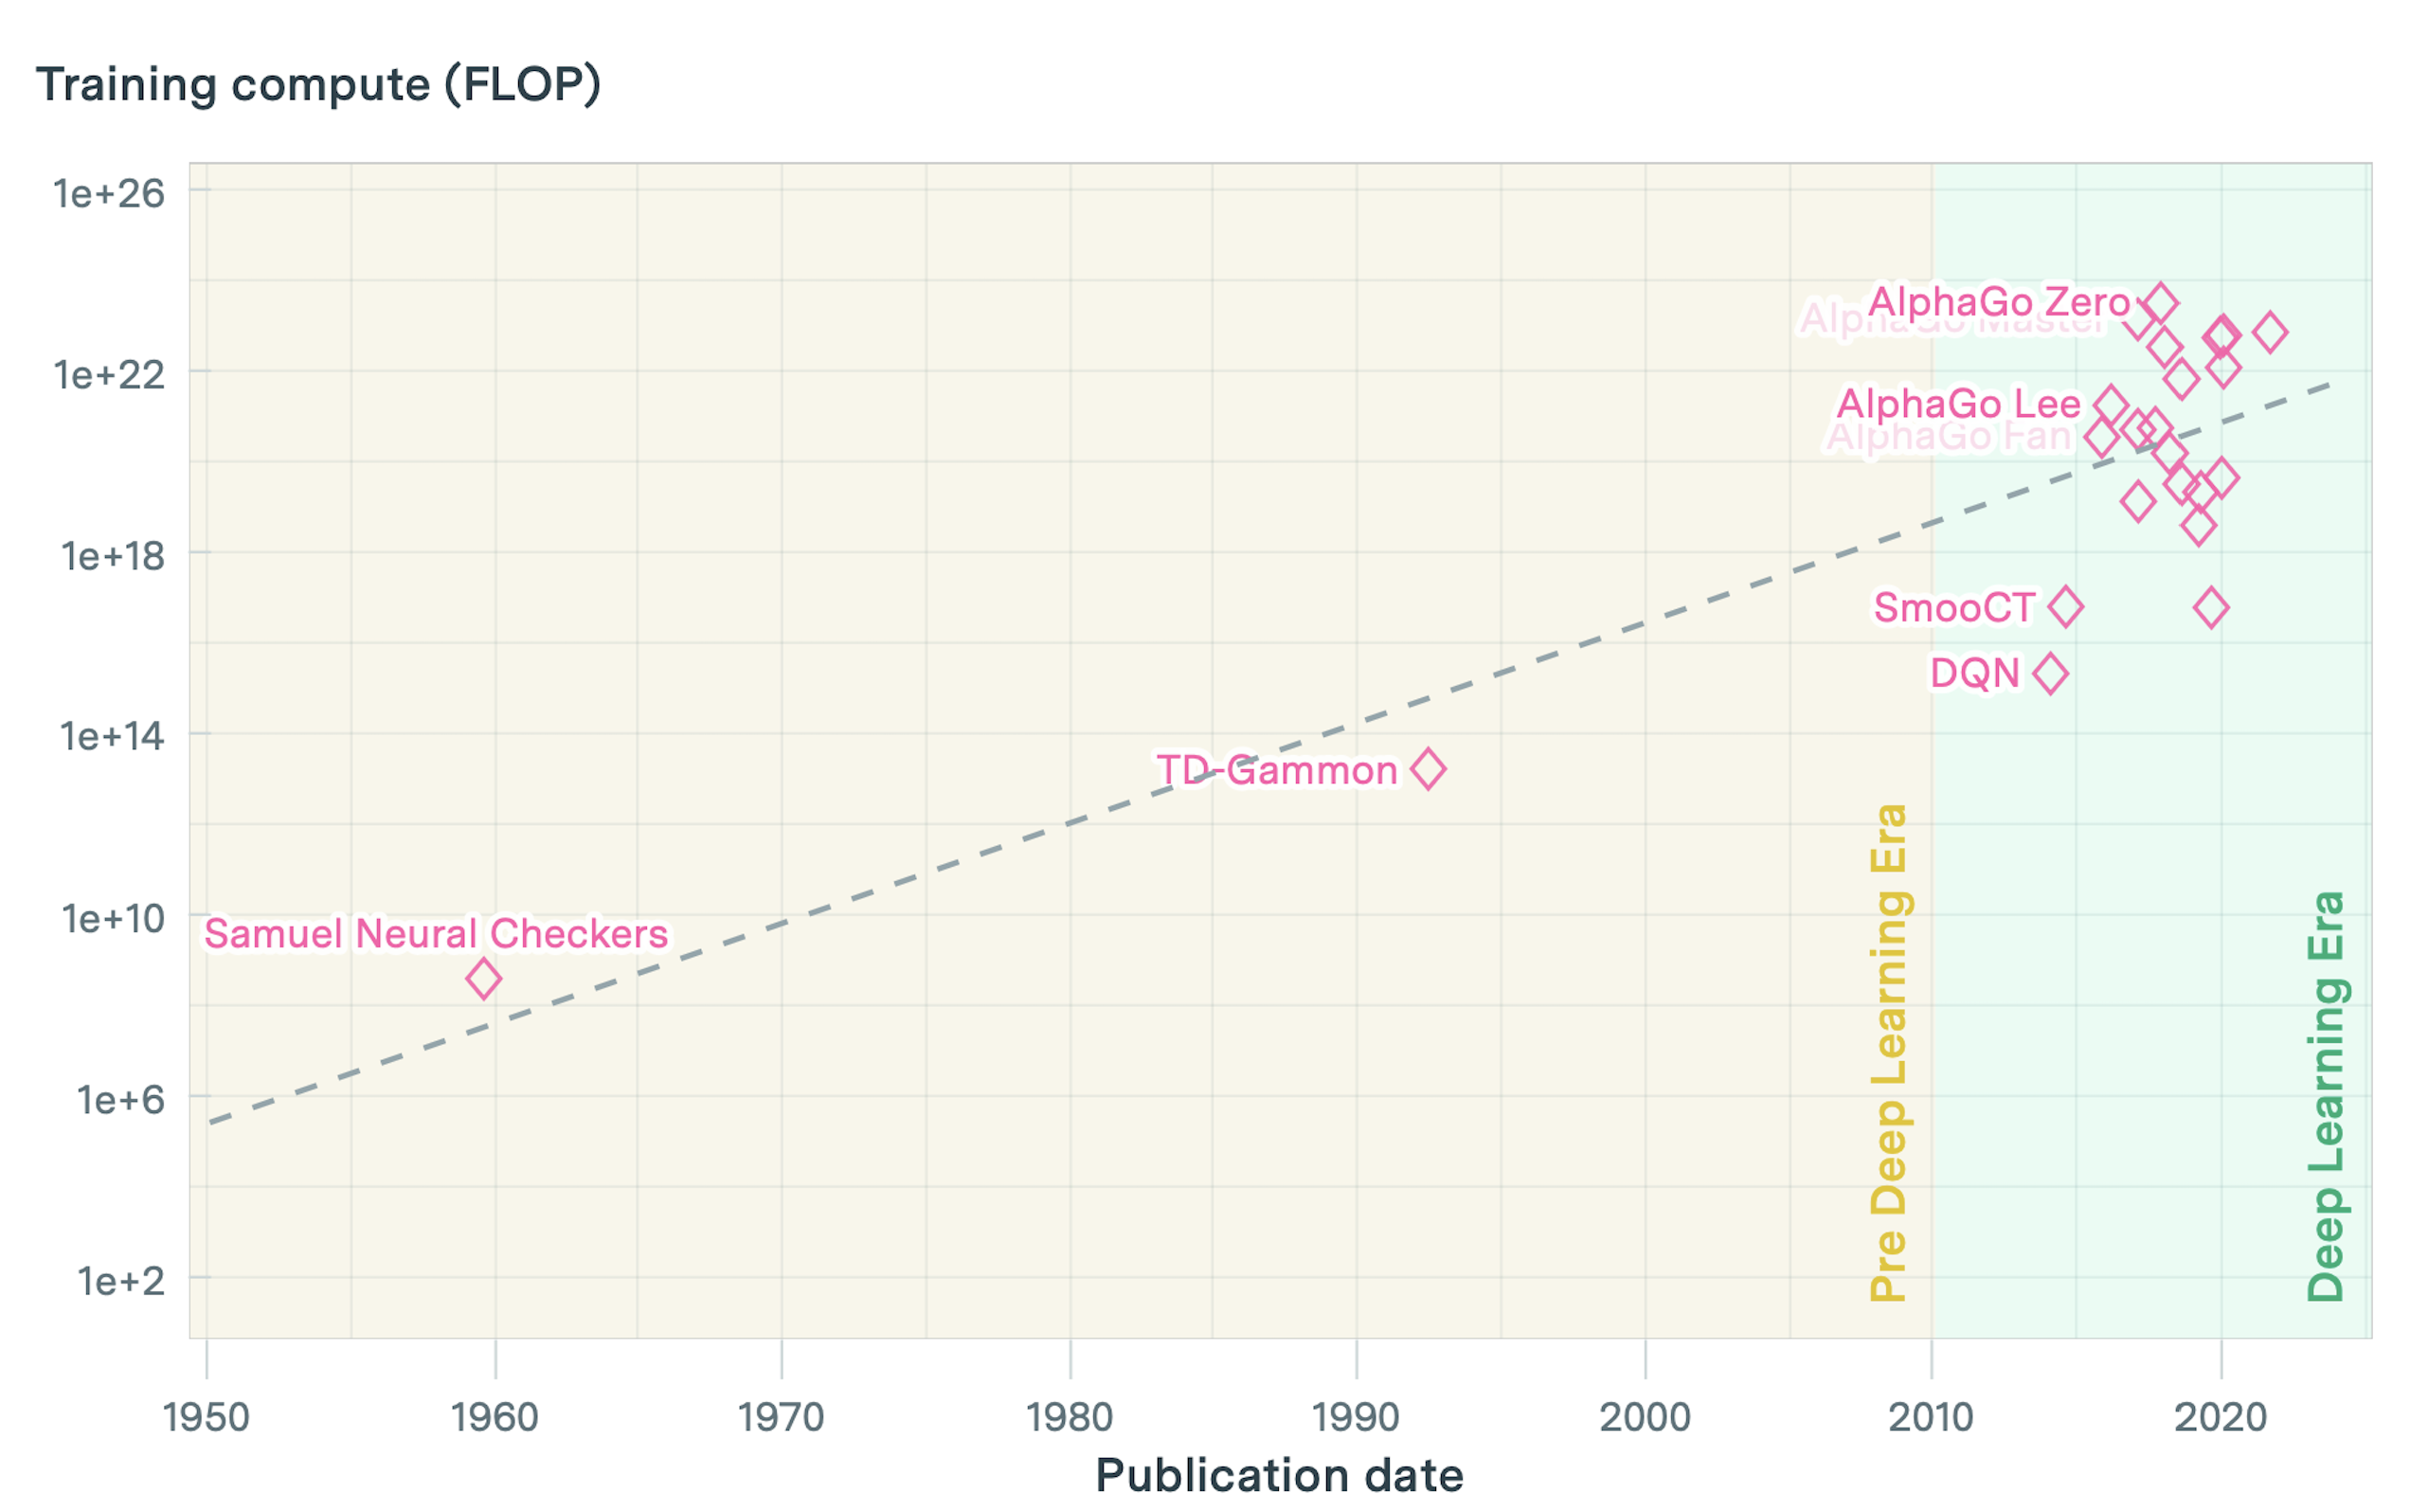
\includegraphics[width=1\linewidth]{images/intro/related_works/game-trends.png}
    \captionsetup{justification=justified, singlelinecheck=false, width=1\linewidth, labelfont=bf}     
    \caption{Exponential growth in training compute requirements for notable AI systems from the 1950s to the present, illustrating the transition from early machine learning to the current Large Scale Era (\textcolor{deepblue}{\cite{epoch2023pcdtrends}}).}
    \label{fig:game-trends}
\end{figure}

\noindent In the domain of complex, high-dimensional grid environments (\textcolor{deepblue}{\cite{eberhardinger2023learning}}), the deployment of deep neural networks is crucial for achieving effective generalization. This requirement is particularly pronounced in the context of the Lux environment, where map heterogeneity is guaranteed by design, where the generation of different environments is seed-dependent. To tackle these issues, (\textcolor{deepblue}{\cite{chen2023emergent}}) proposed a large-scale deep learning solution designed to analyze a wide-ranging, high-dimensional feature space, incorporating diverse environmental attributes like ore maps, ice maps, and distances. They introduced a comprehensive global reward system aimed at recognizing and rewarding any positive developments of an agent, thereby achieving a highly generalized model capable of adapting across various scenarios. This approach necessitated substantial computational resources, specifically requiring an V100 GPU and an additional 600 CPU cores, with the training process extending over multiple phases spanning several days.

\bigskip

\noindent Recent advancements include a deep reinforcement learning algorithm specifically engineered for the complexity of industrial multi-agent systems. Addressing a gap in the research, their approach, the K-nearest multi-agent deep RL (\textcolor{deepblue}{\cite{khorasgani2022knearest}}), is designed to handle scenarios with a fluctuating number of agents and action dependencies among them. Demonstrated through a fleet management simulation by Hitachi, their algorithm showed potential for significant improvements in productivity by optimizing collaborative tasks, such as traffic management, highlighting its applicability in dynamic industrial environments. The paper by (\textcolor{deepblue}{\cite{min2024dynamic}}) presents a novel approach in multi-reward reinforcement learning focused on generating counselor reflections. They introduce two innovative bandit methods, DynaOpt and C-DynaOpt (\textcolor{deepblue}{\cite{min2024dynamic}}), for dynamically adjusting reward weights during training, aiming to optimize text qualities. Their methods outperform existing models, demonstrating significant potential for multi-objective problem decomposition and dynamic rewarding systems. (\textcolor{deepblue}{\cite{Tan_2024}}) propose an adaptive distributed reinforcement learning method for multi-objective optimization in dynamic, distributed Intelligent Transportation Systems. Their approach addresses the challenge of optimizing multiple, potentially conflicting objectives in a changing environment by integrating multi-agent reinforcement learning with adaptive few-shot learning. Tested in an ITS scenario, their algorithm demonstrates superior adaptation and performance across individual and system metrics. (\textcolor{deepblue}{\cite{zheng2024multiagent}}) introduce a novel approach in Multi-Agent Reinforcement Learning (MARL) employing a hierarchy of Reward Machines (RMs) to enhance learning efficiency in cooperative tasks. Their method, MAHRM, adeptly manages complex scenarios with concurrent events and interdependent agents by breaking down tasks into simpler sub-tasks. 


\section{Background}
\label{sec:background}

\noindent Reinforcement Learning (RL) encapsulates all the processes through which agents learn optimal behaviors through exploration and the evaluation of actions based on rewards and penalties. This framework excels in single-agent, single-objective optimization scenarios because it directly aligns an agent's learning process with the maximization (or minimization) of a specific goal, enabling the agent to iteratively refine its strategy towards achieving optimal performance in well-defined environments (\textcolor{deepblue}{\cite{Lee_2020}}). Exploring advanced Reinforcement Learning topics necessitates a solid grasp of the fundamental RL concepts due to the technical complexity of the field. Specifically, Policy Optimization algorithms, which extend basic RL principles, are detailed and form the basis for further discussion. This discourse selectively highlights relevant concepts, omitting details beyond the scope of our research. For a thorough foundational understanding, the seminal work "Reinforcement Learning: An Introduction" by Sutton and Barto (\textcolor{deepblue}{\cite{Sutton1998}}) is an essential reference.

\bigskip

\begin{figure}[htbp]
    \centering
    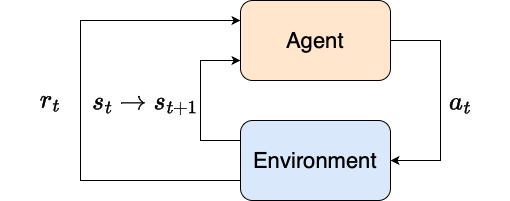
\includegraphics[width=0.6\linewidth]{images/intro/background/rl_simple.png}
    \captionsetup{justification=justified, singlelinecheck=false, width=1\linewidth, labelfont=bf}  
    \caption{The standard representation of the agent-environment control loop depicts the agent as the actuator and the environment as a sensor, sending signals to this actuator. These signals typically consist of reward signals, reflecting the efficacy of the agent's last action $a_t$, and a new environment signal $s_{t+1}$, updated based on the agent's actuator action $a_t$.}
    \label{fig:rl_simple}
\end{figure}

\noindent In reinforcement learning, the foundational components are the \textbdd{environment} and the \textbdd{agents} operating within it. Agents interact with the environment by executing actions informed by \textbdd{observations}, which may vary in terms of their completeness and detail. Based on these observations, the agent decides on \textbdd{actions}, influencing the environment, which can also change independently. The agent aims to maximize its \textbdd{total rewards} over time, known as the return, by learning optimal actions through its interactions. Reinforcement learning techniques enable this learning process by guiding the agent to achieve its goal of reward maximization.

\bigskip

\noindent In deep reinforcement learning, a state $s$ is a detailed representation of the environment, containing all pertinent information, while an observation $o$ provides a subset of this information, possibly omitting crucial details. Deep RL frameworks typically use vectors, matrices, or tensors to model these states and observations. For example, an image might be represented by its RGB values, and a robot's status by vectors of its joint angles and velocities. The environment's \textbdd{observability} is classified based on the agent's access to information: it is fully observed if the agent perceives the entire state, and partially observed if the agent only gets incomplete observations. We will not consider partial observability, since our work focuses only on a fully observed environment (\autoref{sec:environment}).

\bigskip

\noindent The \textbdd{action space} of an environment defines all possible actions an agent can execute. Environments may feature \textbdd{discrete} action spaces, where the choices are finite and distinct (\textcolor{deepblue}{\cite{mnih2013playing}; \cite{SilverHuangEtAl16nature}}), or \textbdd{continuous} action spaces, characterized by actions as real-valued vectors that offer a spectrum of possibilities. This research explores an environment that integrates both discrete and bounded continuous actions (\autoref{sec:environment}; \autoref{fig:lux-actions_ex}).

\bigskip

\noindent Regarding the actions available to the agent, we define the concept known as a \textbdd{policy}. Policies may be \textbdd{deterministic}, implying that, for a given state, the action selected is consistent and not derived from a probability distribution of actions (\textcolor{deepblue}{\cite{Sutton1998}; \autoref{eq:deterministic-policy}}) .

\begin{equation}
    a_t = \mu(s_t)
    \label{eq:deterministic-policy}
\end{equation}

\noindent The chosen action can be \textbdd{stochastic}, derived by sampling from a probability distribution over possible actions (\textcolor{deepblue}{\cite{Sutton1998}; \autoref{eq:stochastic-policy}}).

\begin{equation}
    a_t \sim \pi_{\theta}(\cdot | s_t).
    \label{eq:stochastic-policy}
\end{equation}

\noindent In deep reinforcement learning we are dealing with prameterized policies, which are characterized by their outputs being computable functions reliant on a distinct parameter set, such as the weights inside an \textbdd{artificial neural network} (ANN), that we can adjust dynamically to the modify the actions of the agent via optimization methods. These weights are usually denoted by $\theta$ (\textcolor{deepblue}{\autoref{eq:stochastic-policy}}). In our research, we exclusively focus on stochastic policies to facilitate exploration; hence, discussions on deterministic policies are beyond the scope of this research.

\bigskip

\noindent The two primary stochastic policies implemented in current deep reinforcement learning frameworks are \textbdd{categorical} and \textbdd{diagonal Gaussian policies} (\textcolor{deepblue}{\cite{SpinningUp2018}}). Categorical policies are designed for discrete action spaces. Diagonal Gaussian policies, on the other hand, are appropriate for continuous action spaces. The Lux Environment utilizes discrete and bounded continuous action values within its action space (\autoref{sec:environment}; \autoref{fig:lux-actions_ex}), but for the purposes of simplification, we used a discretization technique known as \textbdd{binning}. This approach significantly improves performance in on-policy optimization (\textcolor{deepblue}{\cite{tang2020discretizing}}), allowing action prediction in continuous domains using categorical policies. These policies serve as classifiers within the action selection mechanisms, utilizing a neural network to process inputs and ending with a linear layer that generates \textbdd{logits} for each possible action. Logits represent the unnormalized scores output by the linear layer, which are then converted into a probabilistic distribution of actions through the softmax function.

\bigskip

\noindent A \textbdd{trajectory} (\textcolor{deepblue}{\cite{Sutton1998}; \autoref{eq:trajectory}}) represents a sequence composed of state-action pairs as experienced within the environment.

\begin{equation}
    \tau = (s_0, a_0, s_1, a_1, \hdots).
    \label{eq:trajectory}
\end{equation}

\noindent Typically, the initial state of the environment is drawn from a \textbdd{starting state distribution} (\textcolor{deepblue}{\cite{Sutton1998}; \autoref{eq:start-state-distrib}}).

\begin{equation}
    s_0 \sim \rho_0(\cdot).
    \label{eq:start-state-distrib}
\end{equation}

\noindent State transitions within an environment are dictated by the environment's inherent dynamics and depend on the previous action executed, represented by $a_t$. These transitions may follow a deterministic or stochastic pattern, as highlighted in (\textcolor{deepblue}{\cite{Sutton1998}; \autoref{eq:transition}}). 

\begin{equation}
    s_{t+1} \sim P(\cdot | s_t, a_t).
    \label{eq:transition}
\end{equation}

\noindent Specifically, the Lux Environment runs under deterministic rules, as detailed in \autoref{sec:environment}, ensuring that each action directly results in a predictable environmental update. Moving forward, we will term trajectories as \textbdd{rollouts}, adopting a standard nomenclature used in RL.

\bigskip

\noindent The reward function, represented by $R$ has diverse notational variations, with a common formulation involving the agent's current state, the action executed in that state, and the subsequent state resulting from the action (\textcolor{deepblue}{\cite{Sutton1998}; \autoref{eq:reward}}).

\begin{equation}
    r_t = R(s_t, a_t, s_{t+1})
    \label{eq:reward}
\end{equation}

\noindent The notation for reward is often simplified to depend solely on the state at timestep $t$, $R(s_t)$, or on both the current state and the recently executed action at timestep $t$, $R(s_t, a_t)$. The objective of the agent is to maximize the total accumulated reward throughout a rollout, denoted as $R(\tau)$ (\textcolor{deepblue}{\cite{Sutton1998}}). However, given the variety of possible returns, this notation can be ambiguous. The first concept of return encountered in the literature is termed the \textbdd{finite-horizon undiscounted return}, which aggregates the rewards collected within a predetermined rollout window (\textcolor{deepblue}{\cite{Sutton1998}; \autoref{eq:reward-undiscounted}}).

\begin{equation}
    R(\tau) = \sum_{t=0}^{T} r_t.
    \label{eq:reward-undiscounted}
\end{equation}

\noindent  Mathematically, the reward may not always converge to a finite value. To address this, the concept of \textbdd{infinite-horizon discounted return} is introduced, which applies a discount factor, $\gamma$ to future rewards. This discounting ensures convergence under suitable conditions. When $\gamma$ is set to 1, it results in the equivalent of an undiscounted return (\textcolor{deepblue}{\cite{Sutton1998}; \autoref{eq:reward-discounted}}).

\begin{equation}
    R(\tau) = \sum_{t=0}^{\infty} \gamma^{t}r_t.
    \label{eq:reward-discounted}
\end{equation}

\noindent The core goal of the agent is to adopt a policy that ensures the maximization of its expected return, regardless of the specific return metric or policy model used. In a deterministic environment, such as the one addressed in our research, the probability function $P(s_{t+1} | s_t, a_t)$ transforms into a deterministic relation $s_{t+1} = f(s_t, a_t)$. This modification indicates that state transitions are directly determined by the current state and action, simplifying the calculation of trajectory probabilities under a given policy $\pi$ (\textcolor{deepblue}{\cite{Sutton1998}; \autoref{eq:prob-func}}).

\begin{equation}
    P(\tau | \pi) = \rho_0(s_0)\prod_{t=0}^{T-1} \pi(a_t|s_t).
    \label{eq:prob-func}
\end{equation}

\noindent Given that the transitions are deterministic, the expectation of the return, $J(\pi)$, remains (\textcolor{deepblue}{\cite{Sutton1998}; \autoref{eq:expected-return}}):

\begin{equation}
    J(\pi) = \int_{\tau} P(\tau | \pi) R(\tau) = \mathbb{E}_{\tau \sim \pi} \text{ }[R(\tau)]
    \label{eq:expected-return}
\end{equation}

\noindent The optimization challenge in reinforcement learning involves identifying the \textbdd{optimal policy} by selecting the argument $\pi$ that maximizes the expected return (\textcolor{deepblue}{\cite{Sutton1998}; \autoref{eq:optimal-policy}}).

\begin{equation}
    \pi^* = \arg \max_{\pi} J(\pi),
    \label{eq:optimal-policy}
\end{equation}

\noindent with $\pi^*$ being the optimal policy.

\bigskip

\noindent \textbdd{Value functions} quantify expected rewards from given states or state-action pairs under defined policies. Value functions estimate the benefit of an agent being in a specific state and play a role, in some form, across nearly all reinforcement learning algorithms (\textcolor{deepblue}{\cite{SpinningUp2018}; \cite{AlMahamid_2021}}). The \textbdd{On-Policy Value Function} calculates the expected reward for being in state $s$ while following a specific policy $\pi$, essentially computing the expected reward across a trajectory $\tau$ (\textcolor{deepblue}{\cite{Sutton1998}; \autoref{eq:value}}).

\begin{equation}
    V^{\pi}(s) = \mathbb{E}_{\tau \sim \pi} \text{ }[R(\tau) | s_0 = s]
    \label{eq:value}
\end{equation}

\noindent The \textbdd{On-Policy Action-Value Function} estimates the value of starting in state $s$, taking an initial arbitrary action $a$, and thereafter adhering to policy $\pi$, providing a measure that parallels the On-Policy Value Function but starts with a specific action $a$ (\textcolor{deepblue}{\cite{Sutton1998}; \autoref{eq:action-value}}).

\begin{equation}
    Q^{\pi}(s, a) = \mathbb{E}_{\tau \sim \pi} \text{ }[R(\tau) | s_0 = s, a_0 = a]
    \label{eq:action-value}
\end{equation}

\noindent \textbdd{Optimal value functions} signify the maximum expected return obtainable from a state $s$ when following the optimal policy within an environment. Conversely, optimal action-value functions indicate the highest expected return achievable by executing an action $a$ in state $s$ and adhering to the optimal policy for all subsequent decisions. The optimal value function is defined as (\textcolor{deepblue}{\cite{Sutton1998}; \autoref{eq:optimal-value}}):

\begin{equation}
    V^{*}(s) = \underset{\pi}{\text{max }} \mathbb{E}_{\tau \sim \pi} \text{ }[R(\tau) | s_0 = s],
    \label{eq:optimal-value}
\end{equation}

\noindent while the optimal action-value function has the following form (\textcolor{deepblue}{\cite{Sutton1998}; \autoref{eq:optimal-action-value}}):

\begin{equation}
    Q^{*}(s, a) = \underset{\pi}{\text{max }} \mathbb{E}_{\tau \sim \pi} \text{ }[R(\tau) | s_0 = s, a_0 = a].
    \label{eq:optimal-action-value}
\end{equation}

\noindent In value and action-value functions, we assume an \textbdd{infinite-horizon discounted return} to ensure convergence. Without discounting, a finite horizon is required to avoid infinite returns, making the concept of expected return meaningless and impractical for RL tasks. In the undiscounted case, incorporating time as an argument is necessary to account for time-dependence. An equally important connection in literature is to define the value function in terms of the action-value function (\textcolor{deepblue}{\cite{Sutton1998}; \autoref{eq:act-val-1}; \autoref{eq:act-val-2}}), highlighting their integral relationship. The value function using the action-value function is defined as:

\begin{equation}
    V^{\pi}(s) = \mathbb{E}_{a \sim \pi} \text{ }[Q^{\pi}(s, a)]
    \label{eq:act-val-1}
\end{equation}

\noindent while the optimal value function using the optimal action-value function has the following form:

\begin{equation}
    V^{*}(s) = \underset{\text{a}}{\text{max }} [Q^{*}(s, a)]
    \label{eq:act-val-2}
\end{equation}

\noindent \textbdd{The Bellman Equations}, crucial to reinforcement learning, establish a recursive linkage between the value of a specific state and the values of its ensuing states. They assert that the optimal policy at any stage matches the optimal policy at all future stages, effectively stating that the value of a state equals the immediate reward plus the expected value of next states under the optimal policy. This principle ensures the consistency and optimality of decision-making across time. Bellman equations use \textbdd{on-policy} notation (\textcolor{deepblue}{\cite{Sutton1998}; \autoref{eq:bellman-value}; \autoref{eq:bellman-action-value}}), calculating state values or action-values based on a specified policy $\pi$ \protect \footnotemark. 

\footnotetext{This notation sometimes leads to confusion with the concepts of on-policy and off-policy learning. In off-policy scenarios, though the equations appear similar, the policy $\pi$ refers to the target policy, whereas data collection follows a different behavior policy $\mu$.}

\begin{equation}
    V^{\pi}(s) = \mathbb{E}_{\underset{s' \sim P(\cdot | s, a)}{a \sim \pi(\cdot | s)}} \text{ } [r(s,a) + \gamma V^{\pi}(s')]
    \label{eq:bellman-value}
\end{equation}

\begin{equation}
    Q^{\pi}(s, a) = \mathbb{E}_{s' \sim P(\cdot | s, a)} [r(s,a) + \gamma \text{ } \mathbb{E}_{a' \sim \pi(\cdot | s')} \text{ } Q^{\pi}(s', a')]
    \label{eq:bellman-action-value}
\end{equation}

\noindent For both value iteration and policy iteration algorithms, the Bellman equations ensure convergence to the optimal policy (\textcolor{deepblue}{\cite{Sutton1998}}), given enough iterations and under certain conditions, such as a finite state space or the presence of a discount factor in infinite horizons. The Bellman equations for optimal value and action-value functions resemble the on-policy framework, yet differ in action selection. Instead of sampling actions a from a state-dependent probability distribution, the optimal framework selects the action that maximizes the future value (\textcolor{deepblue}{\cite{Sutton1998}; \autoref{eq:bellman-optimal-value}; \autoref{eq:bellman-optimal-action-value}}).

\begin{equation}
    V^{*}(s) = \underset{\text{a}}{\text{max }} \mathbb{E}_{s' \sim P(\cdot | s, a} \text{ } [r(s,a) + \gamma \text{ }V^{*}(s')]
    \label{eq:bellman-optimal-value}
\end{equation}

\begin{equation}
    Q^{*}(s, a) = \mathbb{E}_{s' \sim P(\cdot | s, a)} [r(s,a) + \gamma \underset{\text{a'}}{\text{ max }} \mathbb{E}_{a' \sim \pi(\cdot | s')} \text{ } Q^{*}(s', a')]
    \label{eq:bellman-optimal-action-value}
\end{equation}

\noindent In modern RL algorithms, the calculation of a so-called \textbdd{advantage function} plays a crucial role in optimal decision making. The advantage function quantifies the benefit of selecting a particular action $a$ in state $s$ compared to the average result of pursuing other available actions in the same state, given adherence to policy $\pi$ subsequently. The on-policy advantage function, $A^{\pi}(s, a)$, measures the expected benefit of choosing action $a$ compared to following the policy's action distribution in state $s$. This calculation involves subtracting the value function, representing the average benefit of being in state $s$, from the action-value function for a specific action $a$, thus determining a relative improvement over other actions (\textcolor{deepblue}{\cite{Sutton1998}; \autoref{eq:advantage}}). 

\begin{equation}
    A^{\pi}(s, a) = Q^{\pi}(s, a) - V^{\pi}(s)
    \label{eq:advantage}
\end{equation}

\noindent Our research environment (\autoref{sec:environment}) can be formulated as a fully-observable \textbdd{Markov Decision Process}, which is a formal notation frame work for an agent's environment. It is mathematically represented to indicate adherence to the Markov property, meaning that state transitionts do not rely on past history. At any given timestep $t$, the next state $s_{t+1}$ is influenced by the current state $s_t$ and the action $a_t$ taken at that state. In our study, we model our environment as an MDP (\textcolor{deepblue}{\cite{SpinningUp2018}}), represented by the tuple $\langle S, A, R, P, \rho_0 \rangle$, where:

\vspace{-5pt}

\begin{itemize}[itemsep=1pt, parsep=0pt]
    \item $S$ is the set of all possible states, including map features, units, and resources.
    \item $A$ encompasses the entire set of allowable actions, such as digging and moving.
    \item $R : S \times A \times S \rightarrow \mathbb{R}$ is the reward function, devised based on a specific reward scheme.
    \item $P : S \times A \times A_{adv} \rightarrow P(S)$ denotes the state transition probability function. This function is characterized as stochastic in adversarial environments. Transforming the setting to a cooperative scenario, or making the adversary passive, results in a deterministic transition probability of 1.
    \item $\rho_0$ represents the starting state distribution, determined by a controlled seeding method.
\end{itemize}

\noindent Modern RL algorithms fit into a diverse range of domains and applications. Our research focuses on \textbdd{model-free methods}, which operate without an explicit environmental model, restricting the ability to predict state transitions and rewards. This absence prevents the utilization of lookahead or planning techniques to enhance policy learning through forward simulation. Consequently, model-free approaches rely solely on empirical interactions heavily compromising sample efficiency. Moreover, the transferability of models learned from empirical data to real-world scenarios is limited, often requiring substantial computational resources for effective adaptation. 

\bigskip

\noindent In model-free learning, the agent cannot directly access the expected future rewards or the total distribution of the future states and rewards at the start of learning. Instead, these \textbdd{distributions must be approximated} through various methods that explore potential states and rewards within the environment. This concept is central to the multi-armed bandit problem (\cite{Sutton1998}), a form of statistical optimization where the agent must find the optimal balance between exploring the environment to accurately approximate the total distribution of rewards and states and exploiting the environment to maximize reward collection. This framework comprises an evolutionary multi-objective optimization challenge (\cite{Zitzler2012}). Ideally, an agent could achieve a perfect distribution understanding through the law of large numbers with infinite samples and negligible time. However, in practice, resources are finite, and the goal becomes optimizing the utilization of given resources.

\bigskip

\noindent In the case of \textbdd{multi-armed bandits}, imagine a slot machine with $n$ levers, each lever dispensing rewards from a different and unknown distribution. The algorithm's goal is to devise an optimal strategy that balances the initial exploration of each lever — to collect sufficient data for approximating the distribution of rewards — with the exploitation of this data to maximize accumulated rewards by prioritizing levers with higher payouts (\cite{Sutton1998}). The complexity of finding an optimal solution increases with the complexity of the reward distributions, particularly if they are heavily skewed, irregular, or multimodal, as these require more samples to approximate accurately. For example, consider a lever that typically yields no or minimal rewards but, on rare occasions, dispenses the largest jackpot in the country. This scenario would necessitate more extensive sampling compared to a lever offering moderate but consistent payouts, where the reward distribution might closely resemble a uniform distribution.

\bigskip

\noindent Another distinction between algorithms is concerned with what is being learned by the agent, which can be \textbdd{policies}, \textbdd{value functions}, \textit{action-value functions} or the \textbdd{model of the environment}. There are two main approaches to represent model-free reinforcement learning: \textbdd{policy gradient methods} and \textbdd{value-based methods}.

\bigskip

\noindent To properly understand policy gradient methods, it's important to differentiate between an \textbdd{agent} and an \textbdd{entity} in the environment. In scenarios with a single agent, the policy is the learning entity controlling the algorithm while following a policy (\textcolor{deepblue}{\cite{Sutton1998}}). However, in multi-agent systems, it's necessary to distinguish between passive or heuristic entities and learning entities. The definition of an agent in multi-agent systems depends on how rewards are distributed across agents, whether based on global or local information, how experience is divided into multiple trajectories, and how action probabilities, entropies, and advantages are calculated. If an entity in the environment is passive or follows a pre-defined heuristic operation, it's not considered an agent, but rather a passive entity. If the same rewards are distributed to all agents based on a single trajectory using global observation, the agent is considered the \textbdd{orchestrator}. Conversely, when rewards or other computations are allocated at the entity or group level, agents are referenced accordingly to those groups or individual entities. This approach may encompass all entities present on the map as agents, as rewards, advantages, and model updates are computed based on individual trajectories and at the individual level.

\bigskip

\noindent When dealing with multiple agents, the method of credit assignment must also be mentioned. In a cooperative scenario, rewards must reflect not only the individual's achievement but also the shared goals of the entire team in order to drive the agent towards the desired degree of altruistic behavior. By forgoing team-based rewards, the agents might prefer to act in their own self-interest, while not providing them with enough "selfish" rewards could result in their inability to learn basic functions due to the sparsity of the reward feedback. This phenomenon is called the credit assignment problem, and multiple approaches have been theorized for its mitigation. These include the utilization of counterfactual reward baselines (\cite{foerster2017counterfactual}) and forgoing the multi-agent aspect of the scenario entirely with the use of an orchestrator (\cite{chen2023emergent}).


\subsection{Policy Gradient Methods}
\label{sec:Policy-Gradient-Methods}

\noindent Policy optimization algorithms explicitly parameterize the policy by employing a set of parameters denoted as $\theta$. The objective of these algorithms is to optimize these parameters by optimization methods on the objective function, denoted as $J(\pi_\theta)$, which is the total expected return across a given trajectory $\tau$ (\textcolor{deepblue}{\cite{SpinningUp2018}}). Optimization techniques may also focus on maximizing local approximations of this function. These algorithms operate on an on-policy basis, meaning they use data generated from the current policy's actions to calculate updates. The process includes learning a value function approximator, $V_\theta(s)$, for the on-policy value function, $V^{\pi}(s)$, which assists in guiding policy updates.

\bigskip

\noindent To optimize the objective function $J(\pi_\theta)$ via gradient ascent, it's essential to define the concept of the \textbdd{policy gradient}, which represents the derivative of the expected reward with respect to the policy parameters $\theta$. This leads to the formulation of the parameter update rule as follows (\textcolor{deepblue}{\cite{SpinningUp2018}; \autoref{eq:param-update}}):

\begin{equation}
    \theta_{k+1} = \theta_k + \alpha \nabla_{\theta} J(\pi_{\theta})
    \label{eq:param-update}
\end{equation}

\noindent Policy gradient algorithms, including Trust Region Policy Optimization, Proximal Policy Optimization, Recurrent-PPO, and Masked-PPO, form the basis of our research experiments presented. These algorithms utilize distinct update mechanisms, ratios and gradient clipping methods to steer the policy toward optimality (\textcolor{deepblue}{\cite{lehmann2024definitive}}). For implementation purposes, a generalized, computationally viable and numerically stable form of the update rule is adopted from vanilla policy gradient techniques. The derivation of the analytical gradient is beyond the scope of this study and is detailed in Sutton and Barto's book (\textcolor{deepblue}{\cite{Sutton1998}}).

\bigskip

\noindent The complete derivation of the vanilla policy gradient results in an expression representing the expected cumulative sum of the policy's log probability gradients, each weighted by the trajectory's total reward, across all possible trajectories (\textcolor{deepblue}{\cite{SpinningUp2018}; \autoref{eq:policy-gradient}}).

\begin{equation}
    \nabla_{\theta}J(\pi_{\theta}) = \mathbb{E}_{\tau \sim \pi_{\theta}} \left[ \sum_{t=0}^{T} \nabla_{\theta} \text{ log } \pi_{\theta}(a_t | s_t) \underbrace{R(\tau)}_{\text{ total reward }}\right]
    \label{eq:policy-gradient}
\end{equation}



\noindent Given the principle of the law of large numbers (\textcolor{deepblue}{\cite{Athreya2006}}), the expected form of the vanilla policy gradient can be estimated by aggregating a large volume of environment rollouts. By defining this set of rollouts as $D$, where the cardinality of the set is $|D| = N$, the formula for the vanilla policy gradient is accordingly updated for estimation (\textcolor{deepblue}{\cite{SpinningUp2018}; \autoref{eq:policy-gradient-sample}}).

\begin{equation}
    \hat{g} = \frac{1}{|D|} \sum_{r \in D} \sum_{t=0}^{T} \nabla_{\theta} \text{ log } \pi_{\theta}(a_t | s_t) R(\tau)
    \label{eq:policy-gradient-sample}
\end{equation}

\noindent State-of-the-art policy gradient algorithms adopt a refined version of this fundamental gradient update formula in their original implementations. The computability of the gradient of log probabilities of the policies with respect to the parameters, $\theta$, denoted by $\nabla_{\theta} \text{ log } \pi_{\theta}(a_t | s_t)$ has to be ensured (\textcolor{deepblue}{\cite{SpinningUp2018}}). As the sample size $N$ increases, the sample mean more closely approximates the true mean, resulting in a sample estimate with significantly reduced variance.

\bigskip


\noindent In policy gradient methods, a key mathematical caveat involves the updates to the log probabilities of actions being directly proportional to $R(\tau)$ (\textcolor{deepblue}{\cite{SpinningUp2018}; \autoref{eq:policy-gradient}}), which represents the sum of rewards obtained throughout the whole trajectory $\tau$. This methodology may initially appear counterintuitive, as the objective is to condition agent behavior on the future outcomes of their actions, or the rewards accrued subsequent to a specific timestep $t$. By adjusting the vanilla policy gradient equation to utilize a \textbdd{reward-to-go} formulation instead of the total reward function, the policy gradient becomes more stable, achieving lower variance in parallel (\textcolor{deepblue}{\cite{SpinningUp2018}; \autoref{eq:policy-gradient-updated}}).

\begin{equation}
    \nabla_{\theta}J(\pi_{\theta}) = \mathbb{E}_{\tau \sim \pi_{\theta}} \left[ \sum_{t=0}^{T} \nabla_{\theta} \text{ log } \pi_{\theta}(a_t | s_t) \underbrace{\sum_{t'= t}^{T} R(s_{t'}, a_{t'}, s_{t'+1})}_{\text{reward-to-go}} \right]
    \label{eq:policy-gradient-updated}
\end{equation}

\noindent The "reward-to-go" trick significantly enhances the calculation of policy gradients by addressing a specific optimization problem intrinsic in the vanilla policy gradient equation, known as the \textbdd{Expected Grad-Log-Prob (EGLP) Lemma} (\textcolor{deepblue}{\cite{SpinningUp2018}}). This lemma specifies that for a continuous probability distribution $P_0$ over a random variable $x$, when one integrates over $x$, differentiates both sides of the resulting equation, and then applies a log derivative trick, the outcome is the following (\textcolor{deepblue}{\cite{SpinningUp2018}; \autoref{eq:eglp-lemma}}):

\begin{equation}
    \mathbb{E}_{x \sim P_{\theta}} [ \nabla_{\theta} \text{ log } P_{\theta}(x)] = 0
    \label{eq:eglp-lemma}
\end{equation}

\noindent This equation shows that the product of the gradient of log probabilities with any function exclusively dependent on the current state $t$ will also yield zero. This introduces the baseline function, denoted as $b(s_t)$, which, when added to or subtracted from the reward-to-go component in (\textcolor{deepblue}{\cite{SpinningUp2018}; \autoref{eq:policy-gradient-updated}}), does not affect the expected value of the equation.

\begin{equation}
    \nabla_{\theta}J(\pi_{\theta}) = \mathbb{E}_{\tau \sim \pi_{\theta}} \left[ \sum_{t=0}^{T} \nabla_{\theta} \text{ log } \pi_{\theta}(a_t | s_t) \left( \sum_{t'= t}^{T} R(s_{t'}, a_{t'}, s_{t'+1}) - \underbrace{b(s_t)}_{\text{baseline}} \right) \right]
    \label{eq:policy-gradient-baseline}
\end{equation}

\noindent In policy gradient algorithms like PPO, TRPO, A2C, and VPG, the baseline function is set as the on-policy value function $V^{\pi}(s_t)$. Using $V^{\pi}(s_t)$ as a baseline improves stability and convergence but requires neural network estimation. This requires simultaneous updates to both the policy and the value function estimate, an approach found in \textbdd{actor-critic} methods, where the objective is typically defined by the mean-squared-error (MSE) loss (\textcolor{deepblue}{\cite{SpinningUp2018}; \autoref{eq:mean-squared-error}}).

\begin{equation}
    \phi_k = \text{arg }\underset{\phi}{\text{max }} \mathbb{E}_{s_t, \hat{R_t} \sim \pi_k} \left [ \left (  V_{\phi}(s_t) - \hat{R_t}    \right )^{2} \right]
    \label{eq:mean-squared-error}
\end{equation}

\noindent The final generalization of (\textcolor{deepblue}{\cite{SpinningUp2018}; \autoref{eq:policy-gradient}}) can be expressed as the following:

\begin{equation}
    \nabla_{\theta}J(\pi_{\theta}) = \mathbb{E}_{\tau \sim \pi_{\theta}} \left[ \sum_{t=0}^{T} \nabla_{\theta} \text{ log } \pi_{\theta}(a_t | s_t) \Phi_t \right], 
    \label{eq:policy-gradient-general}
\end{equation}

\noindent where the choice for $\Phi_t$ may include \textbdd{total reward} $\left(R(\tau)\right)$, \textbdd{reward-to-go} $\left(\sum_{t'= t}^{T} R(s_{t'}, a_{t'}, s_{t'+1})\right)$, \textbdd{reward-to-go + baseline} $\left(\sum_{t'= t}^{T} R(s_{t'}, a_{t'}, s_{t'+1}) - b(s_t)\right)$ or be determined by alternative approaches, such as the on-policy action-value function (\textcolor{deepblue}{\cite{SpinningUp2018}; \autoref{eq:action-value-function-phi}}):

\begin{equation}
    \Phi_t = Q^{\pi_{\theta}} (s_t, a_t),
    \label{eq:action-value-function-phi}
\end{equation}

\noindent or the advantage function with its refinement, \textbdd{General Advantage Estimation (GAE)}, employed in algorithms such as PPO and its variants, due to the necessity of estimating the advantage, which cannot be directly calculated (\textcolor{deepblue}{\cite{SpinningUp2018}; \autoref{eq:advantage-function-phi}}).

\begin{equation}
    \Phi_t = A^{\pi_{\theta}} (s_t, a_t) = Q^{\pi_{\theta}} (s_t, a_t) - V^{\pi_{\theta}} (s_t)
    \label{eq:advantage-function-phi}
\end{equation}

\subsection{Value-Based Methods}

\noindent Value-based methods aim to estimate the values $V^{\pi}(s)$ or action-values $Q^{\pi}(s, a)$ of states under a policy $\pi$, adopting a strategy to determine these optimal values first (\textcolor{deepblue}{\cite{SpinningUp2018}}). Consequently, these methods develop a deterministic policy optimized for exploitation by choosing actions that maximize expected returns, guided by choosing actions with respect to the greedy policy. RL literature, such as Sutton and Barto's book (\cite{Sutton1998}), heavily focus on explaining a lot these methods, but in our research we only utilized Q-function approximations with deep Q-learning, therefore we will mention the most notable value-based methods. We think its important to go trough these in a minimalistic way, since they help to build up intuititon for more complex approaches:

\vspace{-2pt}

\begin{itemize}[itemsep=1pt, parsep=0pt]
    \item \textbdd{Value Iteration}: a dynamic programming method for finding either the optimal value function $V^{*}(s)$ or the optimal action-value function $Q^{*}(s, q)$ trough solving the Bellman Equations in an iterative way. It has been shown to converge if certain conditions are met  (\cite{dellavecchia}). Requires the model of the world; in particular, knowing $P(s', r | s, a)$ (\cite{Sutton1998}).

    \item \textbdd{Monte-Carlo Methods}: estimate state or action values by averaging the returns from many complete episodes, updating value estimates only at the end of each episode. These methods do not use partial updates or rely on existing value estimates, instead depending solely on the total actual rewards received. Q-tables are used to maintain Q-values troughout the learning process. This makes the methods impossible to scale to very large problems (\cite{Sutton1998}).

    \item \textbdd{Temporal Difference Methods}: due to the high variance associated with Monte Carlo methods, TD-learning introduces \textbdd{bootstrapping}, which updates Q-values using the immediate reward received and an estimate of future rewards, rather than relying solely on the total discounted return $G$. Two renowned methods fit into this category of algorithms: Q-Learning and SARSA (\cite{Sutton1998}).

    \item \textbdd{n-step Methods}: essentially a combination of both trying to find a sweet spot between deep and shallow backups. Introduces the n-step SARSA, n-step Q-Learning algorithms (\cite{Sutton1998}).

\end{itemize}

\noindent Addressing major challenges in Q-learning, such as extremely poor scaling in large environments with vast state and action spaces, \textbdd{function approximation methods} have been developed. Notably, linear function approximation adopts a statistical approach, while deep Q-learning leverages artificial neural networks to estimate \textbdd{Q-values}. Our research primarily focuses on deep Q-learning, but a brief overview of linear function approximation is also beneficial for understanding the broader context of approximation methods in Q-learning. 

\bigskip


\noindent In linear function approximation, the objective is to approximate a value by using a linear combination of features and weights. Specifically for Q-function approximation, this involves representing the state space through a well-defined set of features, each assigned a specific weight. Instead of directly storing state-action pairs, the approach uses feature vectors $f(s,a)$, where each vector has a dimensionality of $n \times |A|$. Here, $n$ denotes the number of features, and $|A|$ represents the total number of possible actions (\textcolor{deepblue}{\cite{valuemethods}; \autoref{eq:feature-vector}}).

\begin{equation}
        f(s,a) = \begin{bmatrix}
        f_1(s,a) \\
        f_2(s,a) \\
        \vdots \\
        f_{n \times |A|}(s,a)
        \end{bmatrix}
    \label{eq:feature-vector}
\end{equation}

\noindent A weight vector of the same size $W$ is assigned to correspond with each feature-action pair. The final Q-value is then calculated as the linear combination of these feature vectors and weight vectors (\textcolor{deepblue}{\cite{valuemethods}; \autoref{eq:q-approx}}).

\begin{equation}
    Q(s, a \text{ | } W) = f_1(s, a) \cdot w_1^a + f_2(s, a) \cdot w_2^a + \hdots + f_n(s, a) \cdot w_n^a
    \label{eq:q-approx}
\end{equation}

\noindent For effective weight updates in linear function approximation, it is crucial to start with a proper initialization technique and an update rule (\textcolor{deepblue}{\cite{valuemethods}; \autoref{eq:q-weight-update-rule}}). Given the linear nature of the model and the convexity of the optimization problem, these factors ensure convergence (\textcolor{deepblue}{\cite{2010Szepesvari}}).

\begin{equation}
    w_i^a = w_i^a + \alpha \cdot \delta f_i(s, a)
    \label{eq:q-weight-update-rule}
\end{equation}

\noindent In deep Q-learning, the task of updating weights and engineering features for a statistical linear function approximator is done by an artificial neural network. This network automatically learns the features through its layers. A significant advantage of this approach is its versatility; the ANN can handle various types of environment representations, including images, gridmaps, videos, and text. The improved update rule becomes the following (\textcolor{deepblue}{\cite{valuemethods}; \autoref{eq:q-weight-update-rule-ann}}):

\begin{equation}
    \theta = \theta + \alpha \cdot \delta \cdot \nabla_{\theta} Q(s, a | \theta)
    \label{eq:q-weight-update-rule-ann}
\end{equation}

\noindent In deep Q-learning, methods like DQN improve stability by using two neural networks: a primary Q network for updating Q-values and a separate target network, whose weights are periodically synced with the Q network, to provide a stable reference for updates.

\subsection{Evolution Strategies}

\noindent Evolutionary algorithms are a specific subset of optimization techniques that find unique applications in reinforcement learning. Though evolutionary algorithms and RL are strictly categorized as distinct subfields, evolutionary strategies are useful for neural network search and optimization, enhancing methods such as deep Q-learning and policy gradient techniques. Despite being less sample efficient than conventional RL algorithms, evolutionary algorithms require less computational resources and are easily parallelizable, leading to improved processing speeds (\textcolor{deepblue}{\cite{Yanes2021}}). 

\bigskip

\noindent Evolutionary algorithms draw inspiration from \textbdd{biological evolution}, utilizing processes such as reproduction, mutation, recombination, natural selection, and survival of the fittest. These mechanisms make them inherently profficient at exploration and optimization tasks. Among these, the \textbdd{genetic algorithm} (\textcolor{deepblue}{\cite{1975Holland}}) is a fairly well-known algorithm, simulating the process of natural selection inspired by Charles Darwin’s theory. However, a significant challenge with genetic algorithms is the encoding of the problem space, which does not always ensure the discovery of the most optimal solution, especially in vast search spaces.

\bigskip

\noindent We utilized a specific domain of evolution, called \textbdd{evolutionary artificial neural networks}, often termed Neuro-Evolution (\textcolor{deepblue}{\cite{Galvan_2021}}). These methods optimize neural network architecture by evolving topologies, connections, activation functions, the number of hidden layers, and even weights until an optimal solution is reached. Neuro-Evolution is particularly valuable in scenarios where domain-specific knowledge is limited, making it challenging to construct an optimal network architecture through conventional means. In our environment, neuroevolution has been employed to systematically explore the optimization space by conducting randomized searches for an optimal policy.

\section{Environment} \label{sec:env}
\label{sec:environment}

\noindent The Lux AI Environment represents a 2D grid platform tailored for Multi-Agent Reinforcement Learning (MARL) research (\cite{chen2023emergent}), designed to tackle challenges in multi-variable optimization, resource acquisition, and allocation within a competitive 1v1 setting. Beyond optimization, proficient agents are tasked with adeptly analyzing their adversaries and formulating strategic policies to gain a decisive advantage (\textcolor{deepblue}{\cite{lux-ai-season-2}}). The environment is fully observed by all agents.

\subsection{Map}

\noindent The world of Lux is represented as a \textbdd{2D grid}. Coordinates increase east (right) and south (down). The map is always a square and has a variable size of 32, 48, 64 or 128 tiles. The (0, 0) coordinate is at the top left. The map has various features, including raw resources (Ice, Ore), refined resources (Water, Metal), units (Light, Heavy), Factories, Rubble, and Lichen. \textcolor{deepblue}{\autoref{fig:lux-map}} shows two possible generations of the game environment, visualizing different block types and resources. In our research, we utilized Lux AI S2 version $2.2.0$ as the engine for our experiments (\textcolor{deepblue}{\cite{luxais2_neurips_23}}).



\begin{figure}[htbp]
    \centering
    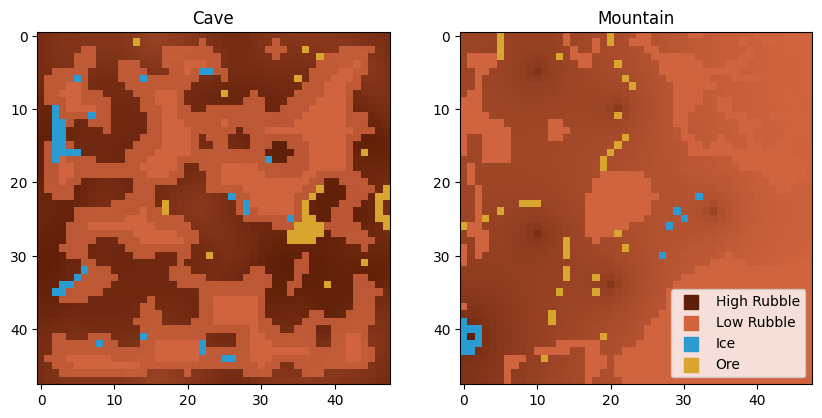
\includegraphics[width=1\linewidth]{images/intro_luxenv/map/resources.png}
    \captionsetup{justification=justified, singlelinecheck=false, width=1\linewidth, labelfont=bf}    
    \caption{Visual Representation of Lux 2D map types which exhibit unique layouts, each generated based on specific seeds \protect\footnotemark. In cave maps, resources are situated inside ravines, while mountain maps, presenting a more challenging terrain, hide resources beneath extensive rubble.}
    \label{fig:lux-map}
\end{figure}

\footnotetext{The maps were generated using seeds $560$ and $788$.}

\subsection{Early Game}
\label{subsec:early-game}

\noindent Each player will start the game by bidding on factory placement order, then alternating placing several factories and specifying their starting resources. Factory placement policies play a crucial role in speeding up the learning process within the game environment. By strategically situating units closer to resources, these policies establish a less cluttered and more conducive proximity environment, thereby promoting faster resource collection. Additionally, the introduction of bidding mechanisms enhances the competitive aspect of the game, compelling players to outbid one another for optimal factory spawn locations. Players are given starting resources for the bidding process. \textcolor{deepblue}{\autoref{fig:lux-map2}} shows map states after concluding the \textbdd{factory placement} and \textbdd{bidding tasks}.

\begin{figure}[htbp]
    \centering
    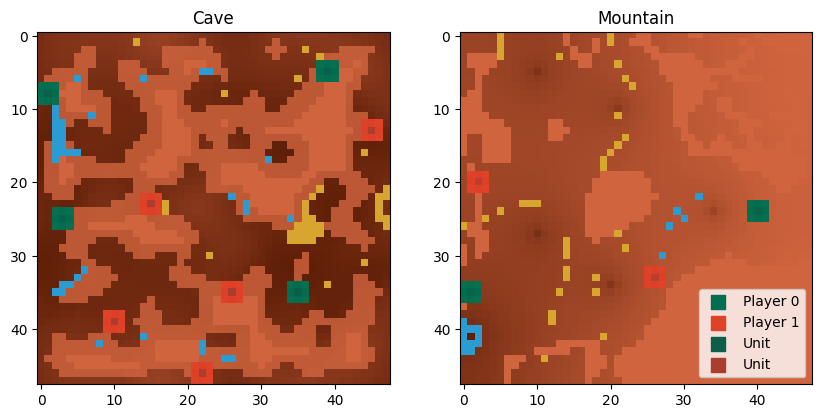
\includegraphics[width=1\linewidth]{images/intro_luxenv/map/factories_units.png}
    \captionsetup{justification=justified, singlelinecheck=false, width=1\linewidth, labelfont=bf}    
    \caption{Visual representation of a random factory placement policy on the two generated maps presented on \textcolor{deepblue}{\autoref{fig:lux-map}}. For further restrictions on factory placement and bidding, please refer to the more in-depth documentation \protect\footnotemark.}
    \label{fig:lux-map2}
\end{figure}

\footnotetext{Advanced specifications available on \href{https://github.com/Lux-AI-Challenge/Lux-Design-S2/blob/main/docs/advanced_specs.md}{GitHub.}}

\subsection{Resources}

\noindent The two kinds of raw resources shown in \textcolor{deepblue}{\autoref{fig:lux-map}}, Ice and Ore, can be refined by a factory into Water or Metal respectively. The raw resources are collected by Light or Heavy units and then dropped off once a unit transfers them to a friendly factory, which then automatically converts them into refined resources at a constant rate. Refined resources are used for growing Lichen, powering factories as well as building more units. For detailed conversion rates and restrictions on transferring resources, please refer to the documentation (\textcolor{deepblue}{\cite{lux-ai-season-2}}).

\subsection{Actions}
\label{subsec:lux-action}

\noindent Units and factories can perform actions at each turn, given certain conditions and enough power to do so. In general, all actions are simultaneously applied and are validated against the state of the game at the start of each turn (\cite{chen2023emergent}). Every turn, players can give an action to each factory and a queue of actions to each unit. Units always execute actions from an action queue, which is limited to a size of 20, while factories directly execute actions. Players can choose to repeat actions for $n$ times, which further complicates the action queue. Submitting a new action queue for a robot requires the robot to use additional power to replace it's current action queue. It costs an additional $1$ power, for light units and an additional $10$ power, for heavy units. For further information regarding action queue updates and repeat handling, please, refer to the documentation (\textcolor{deepblue}{\cite{lux-ai-season-2}}). There are six possible action types that are simplified for easier understanding on \textcolor{deepblue}{\autoref{fig:lux-actions}}.

\bigskip

\begin{figure}[htbp]
    \centering
    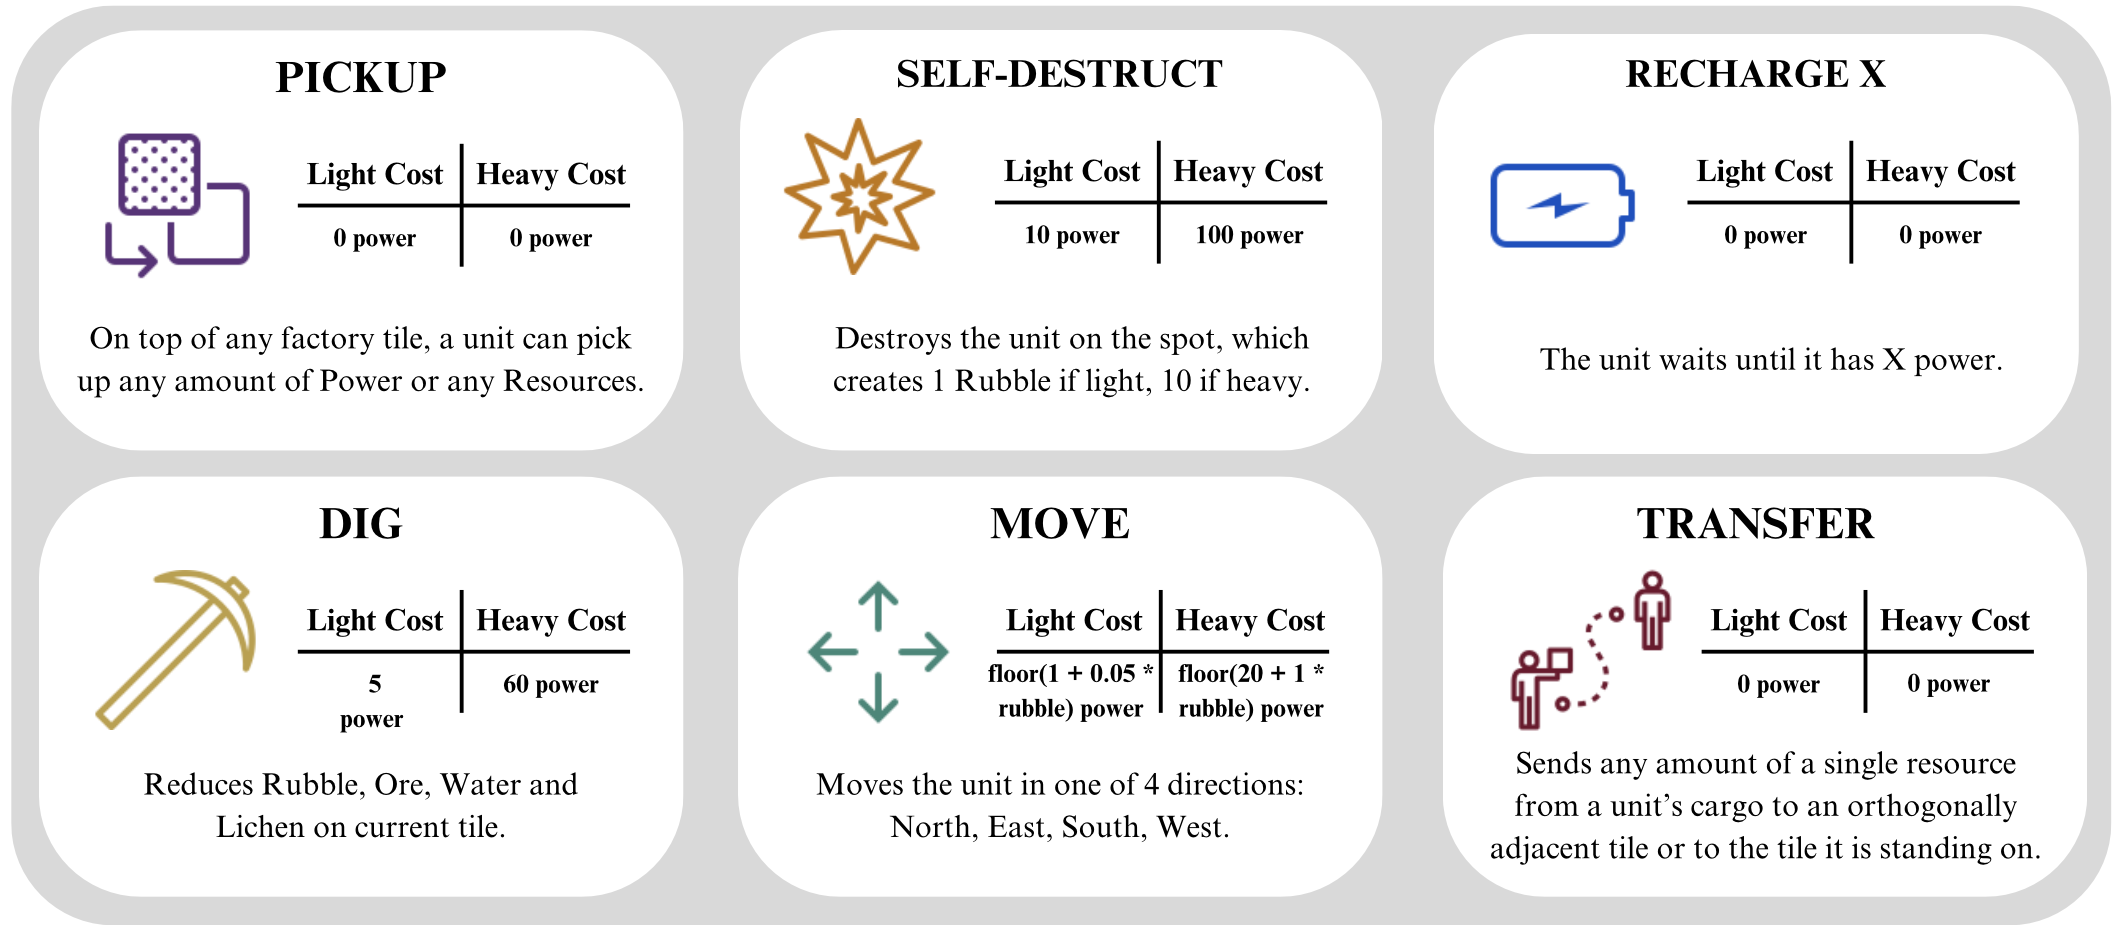
\includegraphics[width=1\linewidth]{images/intro_luxenv/action/action_space.png}
    \captionsetup{justification=justified, singlelinecheck=false, width=1\linewidth, labelfont=bf} 
    \caption{Simplified representation of all possible actions available in the Lux environment. Additional limits and restrictions are applied in the implementation of the engine (\textcolor{deepblue}{\cite{lux-ai-season-2}}).}
    \label{fig:lux-actions}
\end{figure}

\noindent A factory is a building that takes up $3\times3$ tiles of space. Units created from the factory will appear at the center of the factory. Factories can assume passive roles with fixed heuristic action generation, alongside active roles where actions are learned. The action vectors for both factories and units are 1D vectors. Given $n$ units and $m$ factories, predicting action vectors yields matrices of $n\times6$ and $m\times1$, respectively. The response template to the \textbdd{Lux engine} conforms to the format illustrated in \textcolor{deepblue}{\autoref{fig:lux-actions_ex}}.

\begin{figure}[htbp]
    \centering
    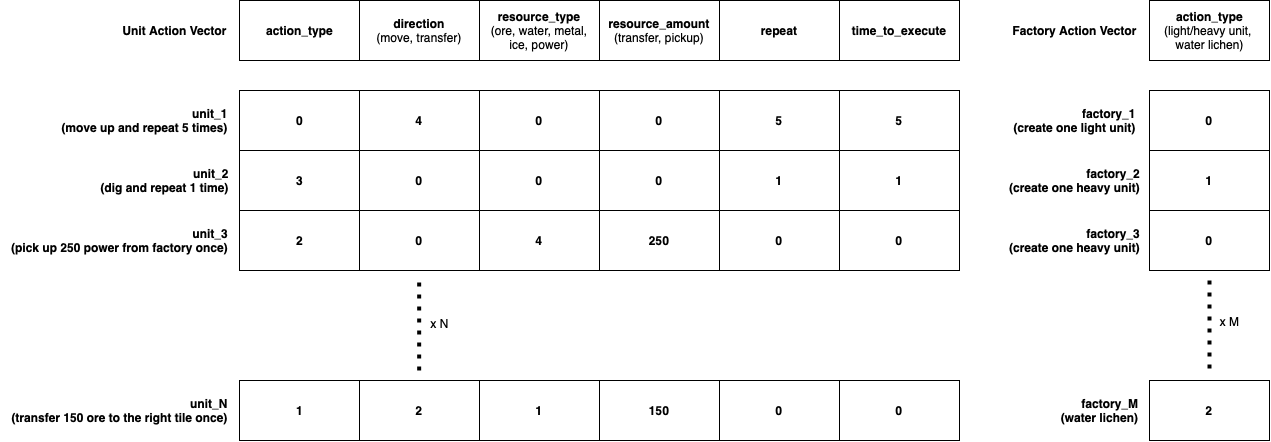
\includegraphics[width=1\linewidth]{images/intro_luxenv/action/action_example.png}
    \captionsetup{justification=justified, singlelinecheck=false, width=1\linewidth, labelfont=bf}
    \caption{Visual example of possible action vectors for both units and factories.}
    \label{fig:lux-actions_ex}
\end{figure}

\subsection{Rubble Dynamics}

\noindent Each square on the map has a rubble value, which affects how difficult that square is to move onto. Rubble value is an integer ranging from 0 to 100. Rubble can be removed from a square by a light or heavy unit by executing the dig action while occupying the square. This environment also has unit collisions. Units which move onto the same square on the same turn can be destroyed and add rubble to the square according to a list of extensive rules in the documentation (\textcolor{deepblue}{\cite{lux-ai-season-2}}).

\subsection{Night Cycles}

\noindent Night cycles are introduced as a complexity measure in the Lux Environment to enhance dynamism and continual change. The environment alternates between \textbdd{day cycles}, which last 30 steps, and \textbdd{night cycles}, which are 20 steps long. This alternation continues until the episode concludes at 1000 steps. During night cycles, the recharging capability of units is stopped, although factories continue to produce power without change (\textcolor{deepblue}{\cite{lux-ai-season-2}; \cite{chen2023emergent}}).

\subsection{Win Condition}
\label{sec:wincondition}

\noindent A game can be resolved in four possible ways:

\begin{itemize}[itemsep=1pt, parsep=0pt]
\item 
In the event that all factories belonging to a player explode, the opposing player is declared the winner.
\item 
If both players lose their last factories in the same step, the game ends in a draw.
\item If each player maintains at least one operational factory, victory in the Lux AI environment is determined by the quantity of Lichen tiles under their control. Lichen watering serves a dual purpose: establishing victory conditions and generating additional power for factories. Due to the intricate nature of power calculations and lichen watering dynamics, we advise consulting the detailed documentation for further understanding (\textcolor{deepblue}{\cite{lux-ai-season-2}}).
\item If the quantity of owned Lichen tiles match, the game concludes in a draw.
\end{itemize}
\noindent







\cleardoublepage

\chapter{Methods}
\label{ch:meth}

\noindent In this chapter, we would like to introduce the different methods utilized in our experiments. We will begin in \autoref{sec:single-unit-testbench} with the specification of our initial trials in a simplified \textbdd{single unit} environment, where we could study different reinforcement learning algorithms without the complexity of multiple agents. Next, in \autoref{sec:monolithic-approach} and \autoref{sec:hybrid-approach} we present two different approaches towards multi-agent control, namely \textbdd{monolithic} and \textbdd{hybrid} architectures. The section on the \textbdd{hybrid approach} contains the definition of our novel \textbdd{trajectory separation} technique.

\section{Single Unit Testbench}
\label{sec:single-unit-testbench}

\noindent We started with a benchmarking study to assess the performance of various RL algorithms within a standardized environment to identify the optimal algorithm for our purposes. We utilized \textbdd{OpenAI's Gym} (not Gymnasium at the time) package (\textcolor{deepblue}{\cite{1606.01540}}) for compatibility with the Lux package and \textbdd{PettingZoo} (\textcolor{deepblue}{\cite{terry2021pettingzoo}}) for environment parallelization. To access state-of-the-art RL algorithms, we conducted our simple benchmarking study using \textbdd{Stable Baselines 3} (\textcolor{deepblue}{\cite{stable-baselines3}}), a reliable collection of reinforcement learning algorithms implemented in \textbdd{PyTorch}. This toolkit provided us with a unified framework for all included algorithms and offered subprocess-level vectorization through Python's \textbdd{Ray} (Ray/RLlib) framework (\textcolor{deepblue}{\cite{moritz2018ray}}), \textbdd{TensorBoard} support (\textcolor{deepblue}{\cite{abadi2016tensorflow}}), and easy out-of-the-box usability. Another significant advantage of Stable Baselines 3 is the fidelity of its implementation to the original specifications in the respective research papers, which meant that only minimal parameter adjustments were necessary for usage. Due to hardware constraints, specifically the availability of only eight logical CPU cores on our local machine, we were limited to running a maximum of eight parallel environments through subprocess-level vectorization.


\subsection{Heuristic Bidding and Factory Placement}
\label{subsec:single-bidding-factory}

\noindent For our testbench, we simplified the problem space to focus on a \textbdd{single-unit scenario}. This involved implementing a straightforward factory placement policy, a basic bidding system, and a simplified controller and action space for our agent. We also employed substantial \textbdd{reward shaping} to focus the agent's learning on a specific task, which was then used for evaluation.

\bigskip 

\noindent The factory placement policy utilized a comprehensive \textbdd{heuristic search} for simplicity, gathering potential spawn positions and identifying areas with high Ice presence. By searching through the ideal locations iteratively, the policy strategically positioned the factory adjacent to Ice clusters within a $3 \times 3$ grid. To completely remove the impact of bidding dynamics in adversarial settings, we adopted a strategy of bidding the minimum required resources while ensuring the opposing agent bid zero. This approach guaranteed us that we started factory placement with the maximum amount of resources possible \protect\footnotemark.

\footnotetext{Our goal was to neutralize the competitive element of the game for this benchmarking study, focusing instead on assessing algorithms through their proficiency in exploration and resource gathering rather than their ability to outperform an adversary.}

\subsection{Actions}
\label{subsec:single-environment}

\noindent In our study, we simplified the game dynamics by converting the factory into a non-learning, heuristic entity. It produced a single Heavy unit at the start of the episode, after which it played no further role, effectively circumventing complications associated with varying entity counts in reinforcement learning settings. Furthermore, we disabled the construction of Lichen, as its contribution to performance metrics — the agent's efficiency in exploring the map and securing necessary resources for the factory — was negligible. Here, therefore, when we use the term \textbdd{agent}, we specifically mean the policy used by the Heavy unit present on the map. This approach, by confining our action space to a singular Discrete action space for one unit, made integration with Stable Baselines 3 easier by ensuring a consistent, discrete-variable-only action space.

\begin{figure}[htbp]
    \centering
    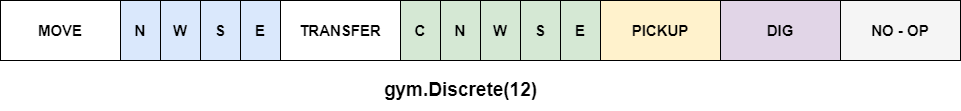
\includegraphics[width=1\linewidth]{images/methods_singleunit/action/controller.png}
    \captionsetup{justification=justified, singlelinecheck=false, width=1\linewidth, labelfont=bf} 
    \caption[]{The action space inside our controller included movements in four cardinal directions, transfers to four cardinal directions and center \protect\footnotemark, pickup, digging, and a no-operation action for debugging.}
    \label{fig:controller}
\end{figure}



\footnotetext{Transfer amount was set to the maximum available resource in cargo, circumventing binning or continuous bounded variables. The same rule applies for pickup actions as well.}


\noindent \textcolor{deepblue}{\autoref{fig:controller}} illustrates the action space adopted for our benchmarking analysis. We excluded certain operations available in the engine, including self-destruct, recharge, action queues (planning), and the transfer of resources other than Ice. The chosen action needed to be formatted to meet the specifications required by the Lux Engine, as detailed in \textcolor{deepblue}{\autoref{fig:lux-actions_ex}}.

\subsection{Observation}
\label{subsec:single-observation}

\noindent Our observation feature space was also designed with simplicity in mind, consisting of only a one-dimensional vector tailored specifically to the task of Ice mining. We intentionally excluded complex data types such as image maps, text, and extensive global information and conducted a small focused \textbdd{ablation study} to make sure the most significant features are present in the input space of the model. As shown in (\textcolor{deepblue}{\autoref{fig:feature-space}}), the features can be broken down into three components. The first section is the unit vector, which contains information about the state of the agent. Namely, the agent's position, class, team, and cargo data. The other two categories are observations about the environment itself. The features included here are vectors pointing towards the closest factory or ice tiles.

\begin{figure}[htbp]
    \centering
    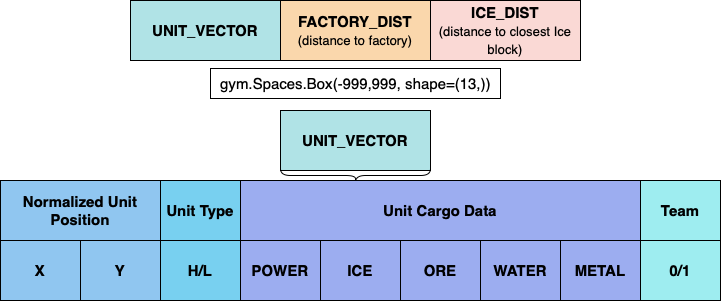
\includegraphics[width=0.8\linewidth]{images/methods_singleunit/observation/feature_space.png}
    \captionsetup{justification=justified, singlelinecheck=false, width=1\linewidth, labelfont=bf} 
    \caption[]{The feature space specifically optimized to maximize Ice collection.}
    \label{fig:feature-space}
\end{figure}

\subsection{Network Architecture}
\label{subsec:single-network}

\noindent Our neural network architecture was also designed with efficient computation and speed in mind, incorporating a small \textbdd{multilayer perceptron (MLP)} with two hidden layers. Each layer uses one \textbdd{linear projection} followed by a \textbdd{ReLU nonlinearity}. The final output layer is a linear projection that maps to the action space of the environment. We evaluated eight state-of-the-art reinforcement learning algorithms: ARS, A2C, DQN, PPO, QR-DQN, R-PPO, TRPO, and MPPO, each utilizing distinct learning approaches and objectives for the agent. Some algorithms employ an actor-critic approach with distinct policy and value heads learned concurrently, while algorithms like DQN and QR-DQN focus on trying to estimate Q-values in different ways for state-action pairs. In contrast, ARS does not learn values, Q-values, or policies directly.

\bigskip

\noindent On-policy actor-critic algorithms often employ \textbdd{separate feature extractors} for the actor and critic components when utilizing simple network architectures like MLPs. This approach is computationally manageable even with relatively small state spaces and has been shown to yield better results (\textcolor{deepblue}{\cite{andrychowicz2020matters}}). However, for more complex models that require a CNN backbone, a shared network architecture should be used since it enables the sharing of critical features between the actor and critic heads while significantly reducing computational overhead. 

\bigskip

\noindent Value-based methods and ARS utilized \textbdd{shared feature extractors}, as they focused solely on learning only Q-values, quantiles, and policy, without the need for distinct learning objectives such as separate value or policy heads. However, not all value-based methods follow this pattern. For instance, Double Deep Q-Learning (\textcolor{deepblue}{\cite{vanhasselt2015deep}}) employs two distinct networks: a primary online network for continuous learning and decision-making, and a separate target network, which is a clone of the primary network. The target network serves as a stable benchmark and is updated less frequently than the primary network.

\bigskip

\noindent It is important to note that while Stable Baselines 3 adheres to the specifications outlined in original research papers (\textcolor{deepblue}{\cite{stable-baselines3}}), these documents often omit significant implementation details, necessitating cautious interpretation of results (\textcolor{deepblue}{\cite{shengyi2022the37implementation}}). Moreover, Stable Baselines 3 incorporates significant, occasionally redundant, code overhead. This issue became more apparent when we used a single-file implementation of the PPO algorithm (\textcolor{deepblue}{\cite{huang2022cleanrl}}), to which we introduced several optimization techniques. For this benchmark study, we are continuing with the SB3 baselines.

\begin{figure}[htbp]
    \centering
    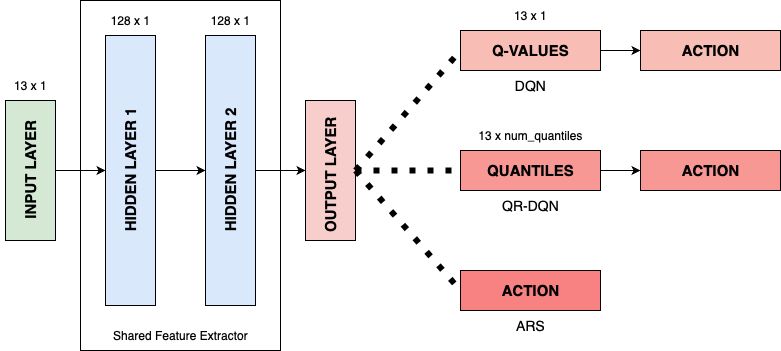
\includegraphics[width=0.8\linewidth]{images/methods_singleunit/net/shared_policy.png}
    \captionsetup{justification=justified, singlelinecheck=false, width=1\linewidth, labelfont=bf} 
    \caption[]{A high-level overview of the neural network layout that employs shared feature extractors used for value-based methods: DQN, QR-DQN, ARS.}
    \label{fig:shared-policy}
\end{figure}

\begin{figure}[htbp]
    \centering
    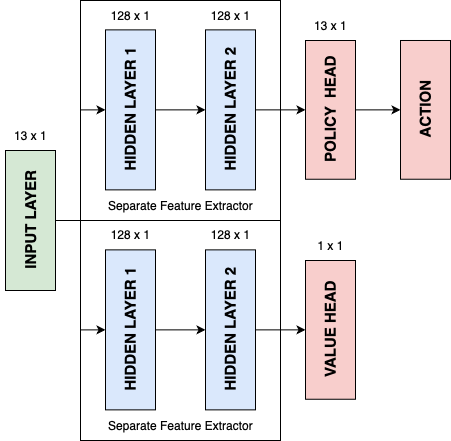
\includegraphics[width=0.6\linewidth]{images/methods_singleunit/net/separate_policy.png}
    \captionsetup{justification=justified, singlelinecheck=false, width=1\linewidth, labelfont=bf} 
    \caption[]{A high-level overview of the neural network layout that employs separate feature extractors used for actor-critic-based methods: A2C, PPO, TRPO, M-PPO, R-PPO. It's important to note that in our implementation of Recurrent Proximal Policy Optimization (R-PPO), we opted for two LSTM layers with a hidden size of 128, instead of using traditional linear projection layers due to the recurrent nature of the algorithm.}
    \label{fig:separate-policy}
\end{figure}


\subsection{Reward Function}
\label{subsec:single-reward}

\noindent Lastly, our reward system was designed with heavy shaping to incentivize two specific behaviors. It encouraged the agent to increase Ice collection and motivated the factory to produce more Water than in the previous round. \textbdd{This 1-step lookback} update-based reward system proved to be an effective method for encouraging targeted behaviors within our model.

\begin{equation}
    r_t = \frac{\Delta \text{ } ice\_dug}{100} + \Delta \text{ } water\_produced
    \label{eq:reward-function}
\end{equation}


\subsection{Training}
\label{sec:single-unit-training}

\noindent We ensured uniformity across all training environments for the algorithms discussed by adhering to the following paradigms:

\begin{itemize}[itemsep=4pt, parsep=0pt]

\item Each algorithm was tested across \textbdd{three trials}, training each from scratch.

\item A \textbdd{specific seed} was manually set for all algorithms and the SB3 torch configuration to maintain consistency across runs.

\item We utilized 8 parallel environments all running on different threads of our CPU.

\item Each environment was configured with a \textbdd{fixed rollout size of 8,192 steps} for policy gradient algorithms, ensuring consistent evaluation across iterations. For value-based methods, the \textbdd{target network was updated every 8,192 steps} to maintain stability. Additionally, each episode was allowed to extend up to 1,024 steps without any truncation. For ARS, updates were calculated at every step.

\item The enemy player was configured as a passive entity without decision-making capabilities; their water count was set to a high level to prevent their factory from being destroyed. Consequently, during each training step, the model was updated using data from \textbdd{only one team}.

\item The predefined hyperparameter sets from the original stable baselines repository were utilized for all algorithms. Batch size was adjusted to 1,024 for all algorithms except ARS, which does not utilize batch updates, in order to accommodate larger updates. Additionally, the \textbdd{number of gradient updates was set to 10} per training phase for all algorithms, with the exception of ARS.

\item A shared feature extractor architecture was employed across all algorithms, consisting of an MLP with two linear layers of size 128 and two ReLU activation layers.

\item All trials were conducted up to a total of \textbdd{1,000,000 steps} (1M).

\end{itemize}


\subsection{Evaluation}
\label{sec:single-unit-eval}

\noindent Our objective in evaluating these novel algorithms was to select one of the eight for scaling up and further assessments across various agent control levels. We aimed to identify an algorithm that aligns best with our specific problem, offers quick performance to speed up research progress, and delivers promising metrics in our benchmark study. The algorithms underwent continuous online evaluation, with the agent interacting with the environment in alternating training and evaluation phases. The criteria for the evaluation phases were as follows:

\begin{itemize}[itemsep=4pt, parsep=0pt]
    \item Every 8,192 steps, four parallel environments were instantiated with a \textbdd{limit of 1,000 maximum episode steps}, the usual game length in the Lux environment.
    
    \item After each evaluation phase, the model state was saved. If it performed better than the current best, the evaluation step was updated and saved.
    
    \item The same stochastic policy used during the training phase was employed for the evaluation phase, meaning that actions were chosen probabilistically rather than greedily at each step.
    
    \item Twelve evaluation episodes were conducted at every phase, resulting in $4 \times 12$ full runs of evaluation episodes to 1,000 maximum episode steps.
    
    \item \textbdd{Quantitative evaluations} utilized metrics that assessed the agent's performance in the environment, such as \textbdd{ice dug} and 
    \textbdd{ice transferred}. These metrics were calculated as the average over the $4 \times 12$ environments.
    
    \item The final quantitative results were averaged over all three trials, meaning the plotted results represent an average over $3 \times 4 \times 12$ evaluation episodes at every 8,192 step interval.
    
    \item Speed (\textbdd{step per second}) was used as an auxiliary metric to measure what could be expected from the algorithms if scaled up.
\end{itemize}

\noindent Our analysis showed conclusive results, identifying Masked-PPO as the most effective algorithm across several metrics: it achieved convergence in the fewest steps, exhibited the fastest performance among the algorithms that actually converged, and its application in multi-agent tasks has been widely documented. Its design allows for straightforward CPU and GPU parallelization due to fixed rollout lengths and minibatch updates. Consequently, Masked Proximal Policy Optimization (M-PPO) will be the primary focus of our subsequent research, while other algorithms may be revisited in future studies.

\section{Multi Agent Environment}
\label{sec:multi-agent-environment}

\noindent Having \textbdd{more than one non-heuristically controlled entity} brings up the question: What do we call an agent? The team of entities, or the entities that make up that team? The Lux Environment (\autoref{sec:environment}) presents a unique challenge in multi-agent control due to its diverse entity types: factories and units. These entities have distinct action spaces and characteristics. Units can be further categorized into light and heavy units, each with different strengths and weaknesses. Units are created by the factories, which further complicates the situation since the \textbdd{number of entities depends on the entities' actions} themselves, and these numbers are \textbdd{constantly changing}.

\bigskip

\noindent In our work, we explored various agent-control approaches, mainly \textbdd{centralized} architectures, where a single pass through the model is responsible for selecting actions for the entire team, turning the multi-agent scenario into a single-agent problem where each controllable entity becomes part of a complex composite action space. One of such implementations is our \textbdd{monolithic approach} (\autoref{sec:monolithic-approach}), where the agent makes decisions for every entity based on a global observation. However, as we will later discuss, this method requires the agent to \textbdd{interpret the entire game state}, which is particularly challenging in highly dynamic environments such as Lux. The complexity of this environment highlights the limitations of existing approaches and the need for a new, more adaptable solution.

\bigskip

\noindent Instead of using a single pass through a centralized model, another option would be to generate actions for every entity individually, based on their own observations. Generating a single entity's action massively reduces the required complexity of the network. Furthermore, we can treat each entity as a \textbdd{separate, parallel environment trajectory}, increasing the train examples collected from one step of the environment. Solutions for PettingZoo ({\cite{terry2021pettingzoo}}) multi-agent environments have been successfully trained with similar approaches using SuperSuit (\cite{SuperSuit}). However, \textbdd{changing agent numbers} poses a problem for such implementations. In our case, factories can explode throughout the game, and units are frequently destroyed or created, making existing multi-agent training solutions obsolete for our use case because they assume a constant number of agents throughout the episode. Additionally, training with on-policy methods requires \textbdd{careful tracking of their trajectories} and creates \textbdd{constantly changing batch sizes} if we treat every agent as a separate observed step. The Lux Environment can have hundreds of units active simultaneously. Storing observations and calculating actions for each unit and factory \textbdd{hinders performance at both training and inference}. For these reasons, we have not explored full multi-agent control. Instead, we used what we call a \textbdd{hybrid approach} (\autoref{sec:hybrid-approach}), which uses a \textbdd{centralized decision-maker} while allowing \textbdd{individual control} of units and factories based on both \textbdd{local and global information}.

\section{Monolithic Approach}
\label{sec:monolithic-approach}

\noindent In our monolithic solution, we introduce a \textbdd{central decision-maker} agent, serving as the exclusive learning entity with oversight over entities that provide information but lack \textbdd{direct influence} on the whole learning process. This framework enables the central decision-maker to supervise all units on the map concurrently, leveraging a global trajectory and reward system for updates. To tackle the challenge of fluctuating numbers of learning agents (\cite{piccoli2023control}; \cite{SuperSuit}), such as factories or units, we implemented a \textbdd{single-trajectory approach} for each episode. This method ensures fixed episode lengths, independent of factors like unit deaths or creations, resulting in a singular termination flag at the conclusion of each episode.

\bigskip

\noindent In our context, \textbdd{direct influence} refers to the scenario where the actions of a single entity directly impact the central decision-maker. However, in the case of the monolithic approach, this direct influence does not occur. Instead, the central brain only perceives global changes in the environment without attributing them to specific agents. We refer to this as \textbdd{indirect influence} on the learning agent. This distinction significantly simplifies the functioning of the learning agent. For instance, when there is a positive change in the environment, such as ice collection, it is reinforced without the need to identify which agent was responsible for the action.

\bigskip

\noindent In our approach, we utilize a single actor and a single critic, forming a \textbdd{single-task learning setup} (\cite{eysenbach2023connection}; \cite{gai2024singletask}; \cite{mysore2022multicritic}) that optimizes a unified global objective. The single actor generates actions for every pixel on the map, creating a global action tensor that encompasses the entire map. From the raw observations, we filter out pixels containing units and factories to form a tensor of shape $M\times|A|$, where $M$ is the number of factories and units, and $|A|$ represents the size of the action space. Similarly, the single critic approximates the singular value of the entire game state. This is what we refer to as a \textbdd{monolithic framework} for PPO: it includes global observations, a single decision maker, a single global trajectory for every episode, a global reward system, a single actor generating a global action tensor, and a single critic evaluating the global state of the game.

\subsection{Environment}
\label{subsec:mono-environment}

\noindent There were minor changes to the environment and learning setups compared to \autoref{sec:single-unit-testbench}. We expanded the action space to include the \textbdd{recharge action} for units and \textbdd{three additional factory actions}: light unit building, heavy unit building, and lichen watering. This adjustment increased the original discrete action space (\autoref{subsec:single-environment}) from 12 to 16. Additionally, we implemented more rigorous action masking, which restricted units from transferring resources to enemy units and factories, prevented out-of-bounds movements, and limited factory unit generation.

\bigskip

\noindent We reduced the episode length during the training phase to 256 steps to \textbdd{fit a broader range of data within the same number of training examples}. This adjustment was driven by the observation that the environment dynamics stabilize after a certain number of steps, especially when the goal is to sustain the factories. Given the relatively straightforward strategy of mining ice and transporting it to the factory, the mechanics remain largely consistent throughout the match. By shortening the episode length during training, we were able to parallelize more environments, resulting in accelerated training.

\subsection{Heuristic Bidding and Factory Placement}
\label{subsec:heur-bidding-factory}

\noindent In our experiments, we aimed to  \textbdd{minimize variance between environments} by employing heuristics for the bidding and factory placement phase (\autoref{subsec:early-game}). Given that bidding reduces starting resources, leading to faster factory depletion, we consistently bid with zero. To optimize ice supply to factories, we identified locations where the \textbdd{adjacency of ice to factories is maximal}. \textbdd{Gaussian filtering} (\cite{gaussianfilter}) techniques were applied to the board to smooth out data, emphasizing nearby points and reducing noise. Gaussian filtering is a method that smooths out data, like images or, in our case, an observed matrix of the board, by giving more importance to nearby points in a \textbdd{bell-shaped distribution}, reducing noise and sharp transitions. This effectively causes the values on the board to spread out in an area, indicating how far away a tile is from other relevant tiles  as shown on Figures \ref{fig:grad-image} to \ref{fig:gaussian-rubble}. After applying Gaussian filtering, the smoothed boards are weighted and summed pixel-wise to obtain final scores for each tile. Placement selection is then performed \textbdd{greedily}, with the factory placed on the tile with the highest score among the currently valid placement locations (\autoref{fig:score-map}).


\begin{figure}[htbp]
    \centering
    \begin{minipage}{1\textwidth}
        \centering
        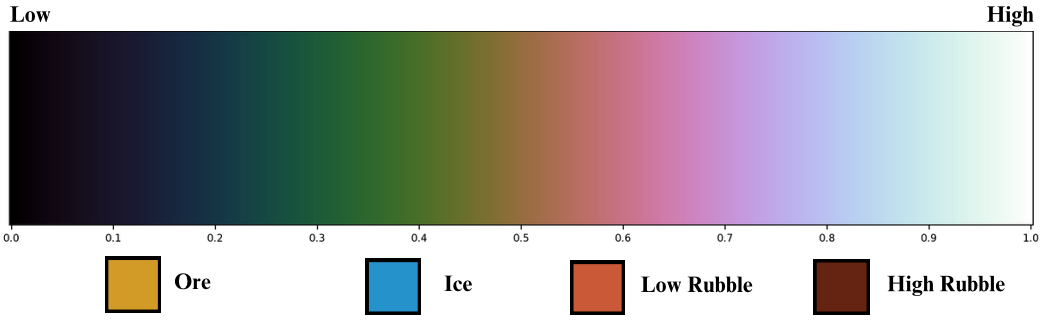
\includegraphics[width=0.8\linewidth]{images/methods_mono/factory_placement/grad.png}
        \captionsetup{justification=justified, singlelinecheck=false, width=1\linewidth, labelfont=bf} 
        \caption{The legend image provided below accompanies subsequent images. It illustrates the original starting map of the Lux environment. The gradient color scheme represents the presence of elements, with lighter colors indicating lower presence and darker colors indicating higher presence. The color mapping for ore, ice, and rubble remains consistent with previous representations (\autoref{fig:lux-map}).}
        \label{fig:grad-image}
    \end{minipage}\hfill
    \centering
    \begin{minipage}{1\textwidth}
        \centering
        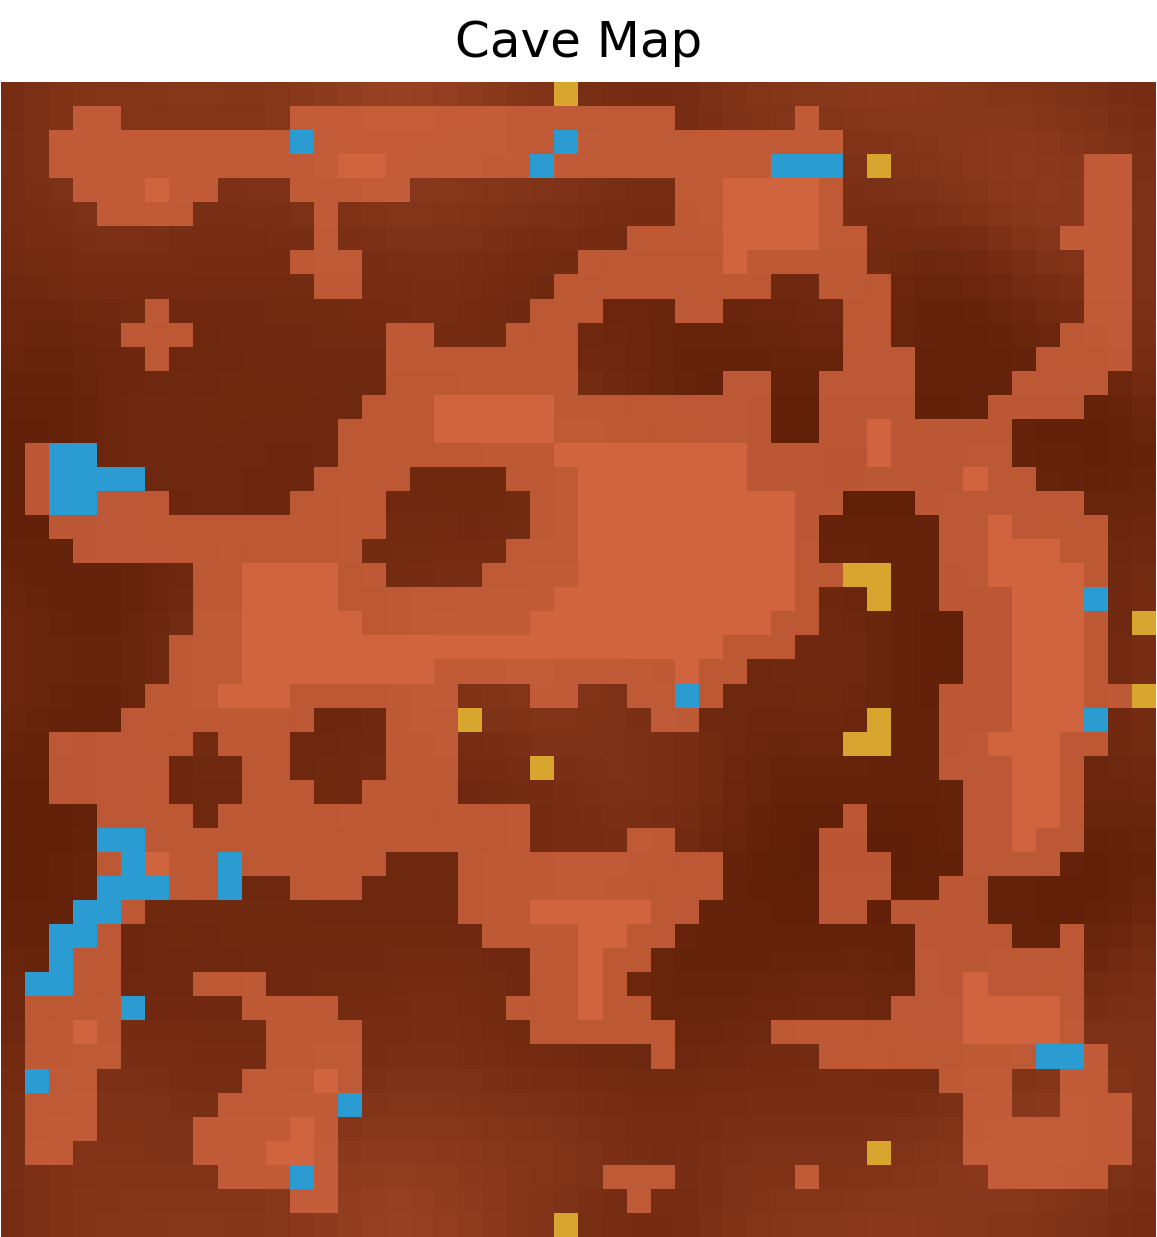
\includegraphics[width=0.3\linewidth]{images/methods_mono/factory_placement/cave_map.png}
        \captionsetup{justification=justified, singlelinecheck=false, width=1\linewidth, labelfont=bf} 
        \caption{Image of the original starting seed of the map without any factories placed on it, generated as the initial step before the bidding phase.}
        \label{fig:grad-map}
    \end{minipage}\hfill
    \vspace{8pt}
    
    \begin{minipage}{0.3\textwidth}
        \centering
        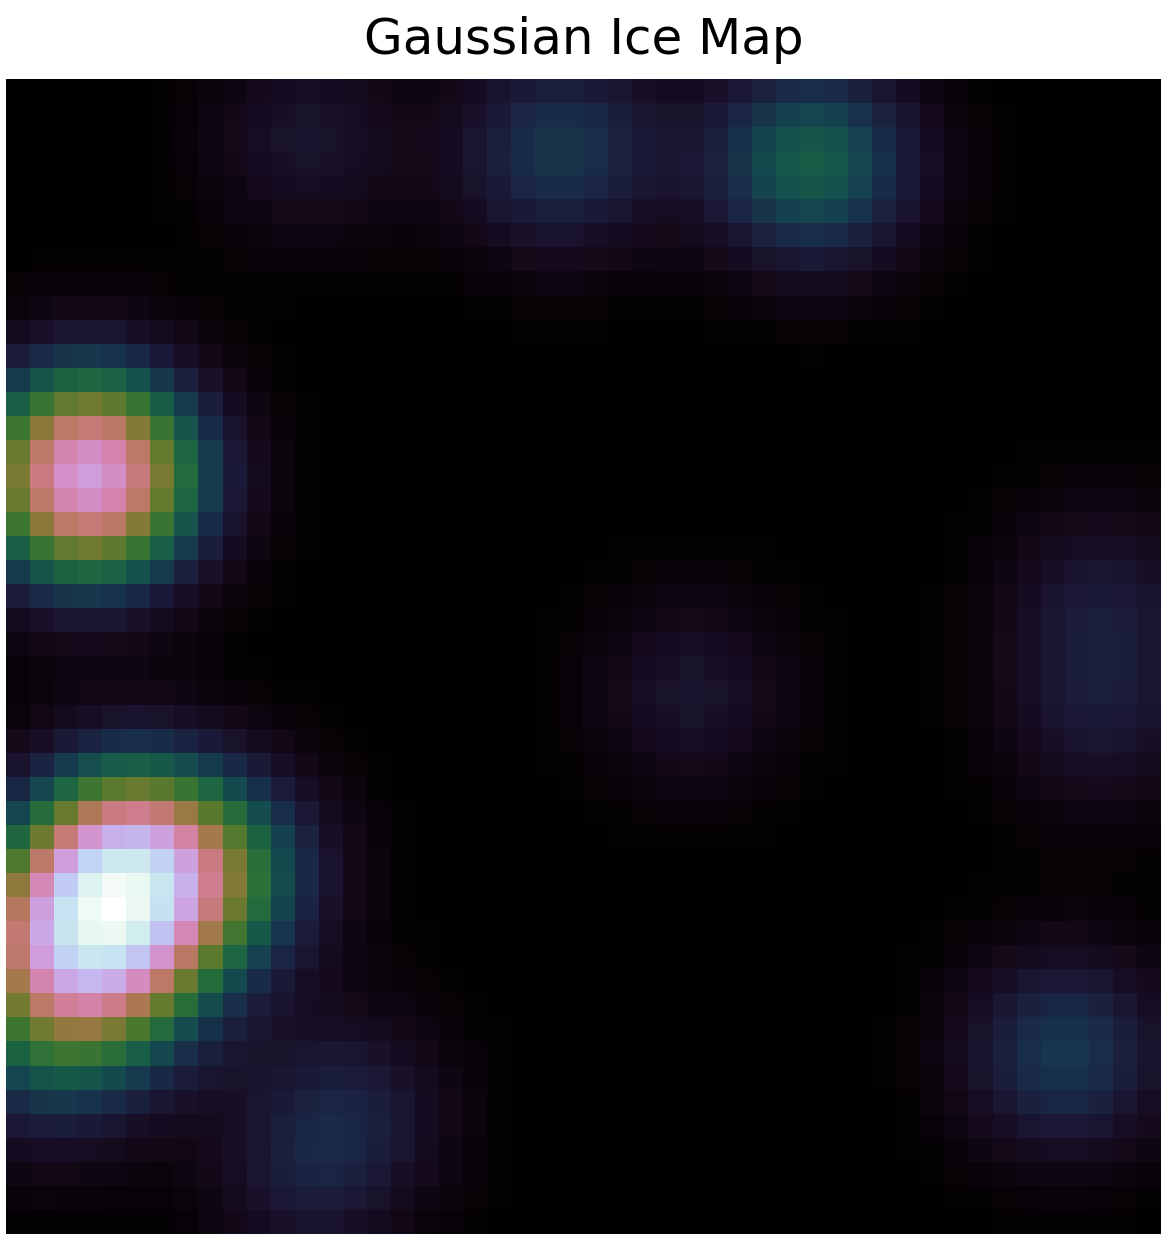
\includegraphics[width=\linewidth]{images/methods_mono/factory_placement/gaussian_ice_map.png}
        \captionsetup{justification=justified, singlelinecheck=false, width=1\linewidth, labelfont=bf} 
        \caption{High presence of ice calculated using our Gaussian filter. Lighter values indicate high-density ice areas.}
        \label{fig:gaussian-ice}
    \end{minipage}\hfill
    \begin{minipage}{0.3\textwidth}
        \centering
        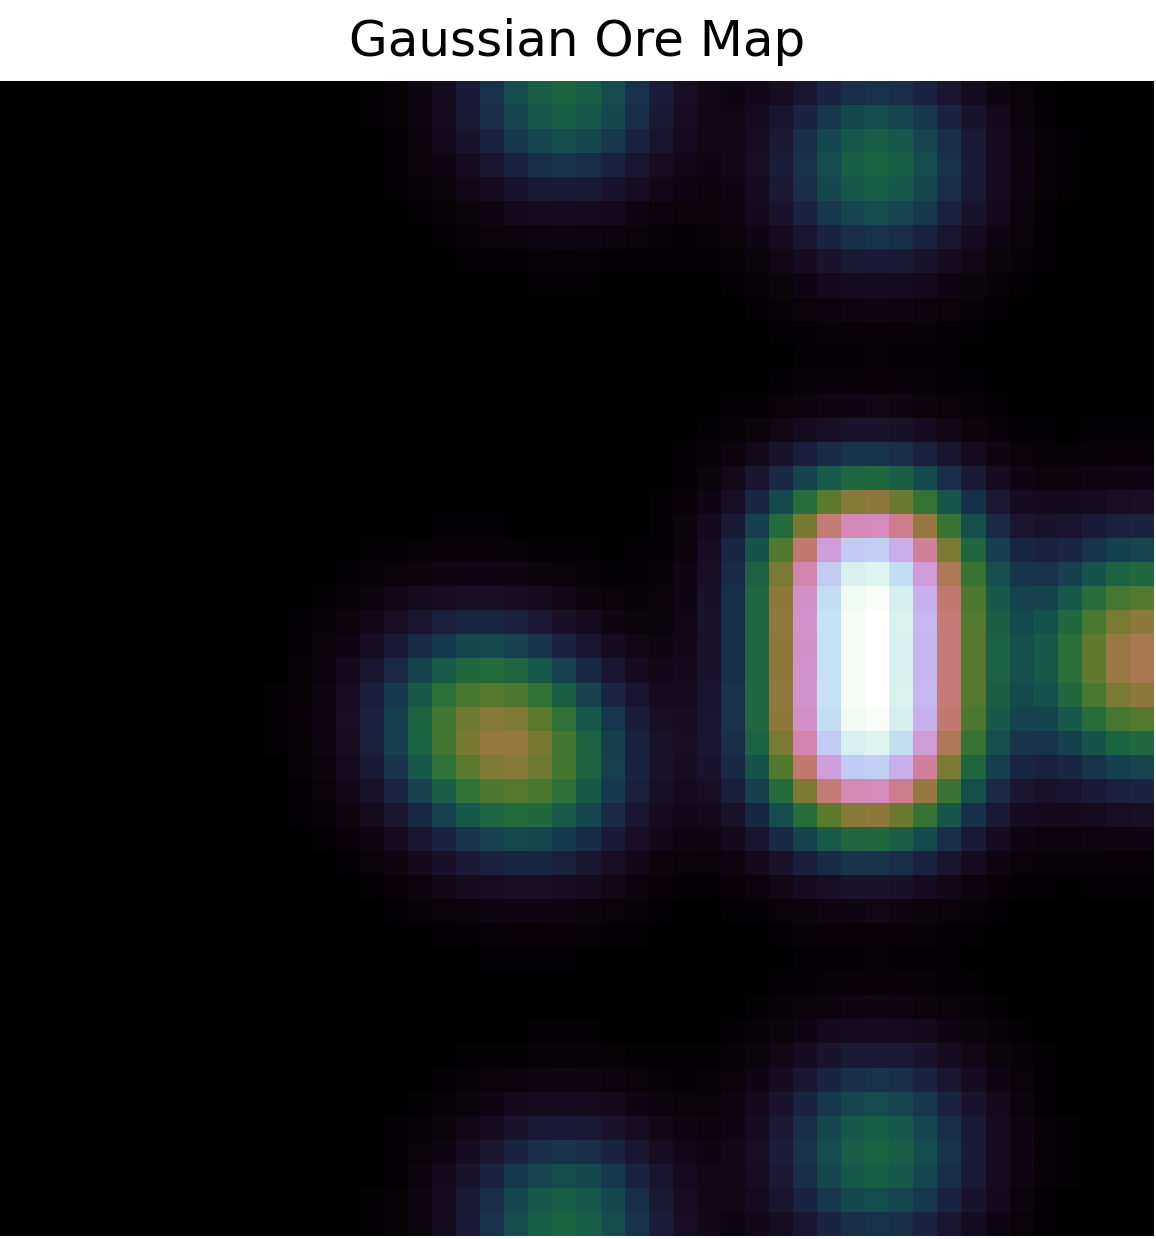
\includegraphics[width=\linewidth]{images/methods_mono/factory_placement/gaussian_ore_map.png}
        \captionsetup{justification=justified, singlelinecheck=false, width=1\linewidth, labelfont=bf} 
        \caption{High presence of ore calculated using our Gaussian filter. Lighter values indicate high-density ore areas.}
        \label{fig:gaussian-ore}
    \end{minipage}\hfill
    \begin{minipage}{0.3\textwidth}
        \centering
        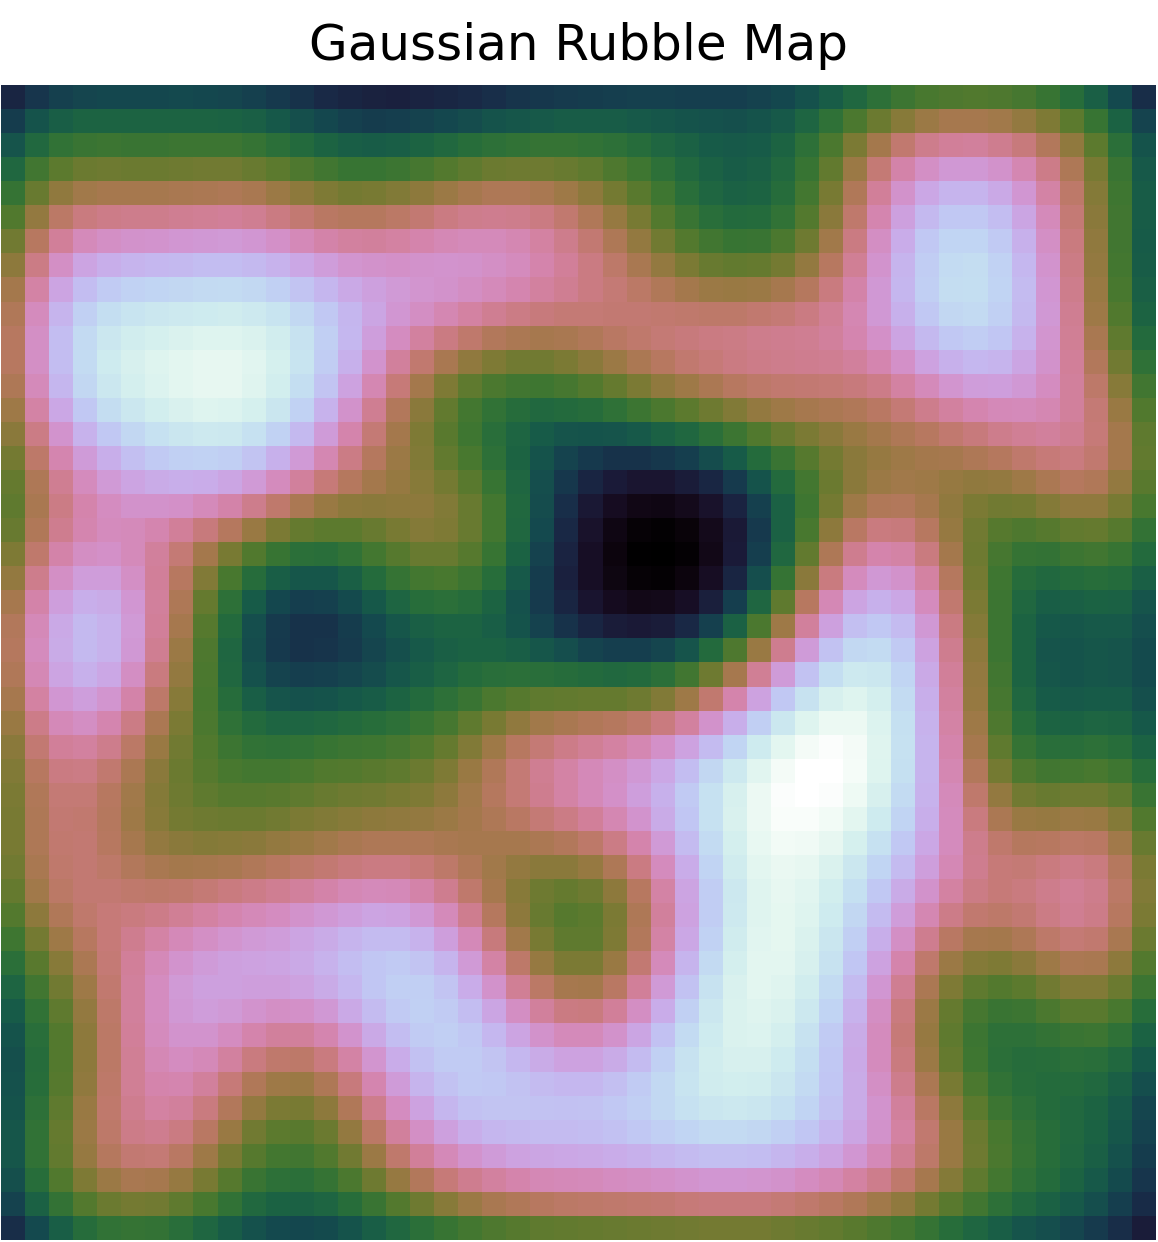
\includegraphics[width=\linewidth]{images/methods_mono/factory_placement/gaussian_rubble_map.png}
        \captionsetup{justification=justified, singlelinecheck=false, width=1\linewidth, labelfont=bf} 
        \caption{High presence of rubble calculated using our Gaussian filter. Lighter values indicate high-density rubble areas.}
        \label{fig:gaussian-rubble}
    \end{minipage}
\end{figure}


\begin{figure}[htbp]
    \centering
    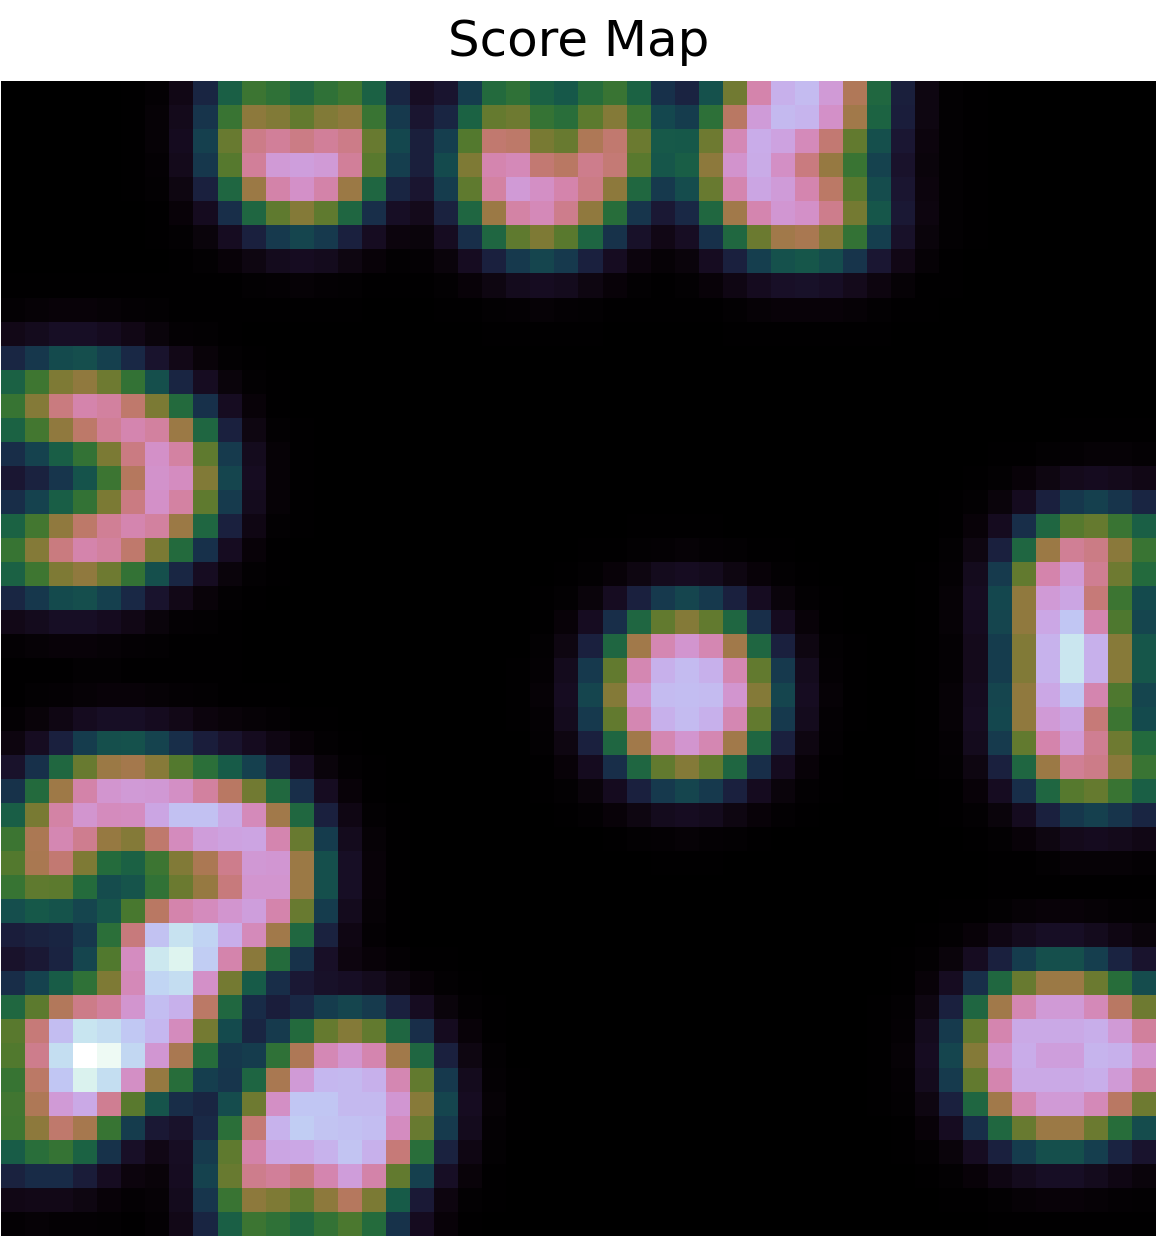
\includegraphics[width=0.3\linewidth]{images/methods_mono/factory_placement/score_map.png}
    \captionsetup{justification=justified, singlelinecheck=false, width=1\linewidth, labelfont=bf} 
    \caption[]{The output of the Gaussian filter algorithm applied to the ore, ice, and rubble maps weighted with possible spawn position maps \protect\footnotemark. Lighter areas indicate the best possible spawn locations.}
    \label{fig:score-map}
\end{figure}

\subsection{Actions}
\label{subsec:mono-actions}

\noindent Utilizing a single actor, we compressed our action space into a single discrete space, accommodating both unit and factory actions. To ensure precise probability calculations and to restrict factory actions for units, and vice versa, we \textbdd{employed invalid action masks}. This essentially led to a theoretical \textbdd{splitting of the action space} into two categories: factory actions and unit actions. Factory actions were masked out for all units, and unit actions were masked out for all factories, with the exception of the no-operation action, which was available to both entity types. Restricting illegal actions within such vast action spaces is crucial for expedited learning. For instance, by forbidding the transfer action when no cargo is available on the unit or when the unit is not adjacent to another unit, or when the factory is not adjacent to the unit, we effectively reduced the range of possible unit actions from 13 to 8 (including move in 4 cardinal directions, pickup, dig, recharge, and no-operation) (\autoref{subsec:lux-action}). Although we did not implement a more complex masking system to limit repeated actions or prevent agents from overlapping, as it would introduce excessive logic and determinism into the game, we aimed for the central decision maker to \textbdd{learn these patterns} rather than explicitly instructing it on all possible negative edge cases. Lichen watering was also excluded for all factories to better align them with the task of preserving their longevity, as watering lichen consumes water, thereby reducing factory lifespan. For global control, our final action space was of size $[16,48,48]$, where each pixel on the map had an assigned action vector, as illustrated in \autoref{fig:action_space_mono}.

\footnotetext{The possible spawn positions are represented by a mask matrix where True values indicate valid spawn positions and False values indicate invalid ones. Invalid positions for factories include those on top of ore blocks, ice blocks, or the very edges of the map. This information is provided and calculated by the Lux AI engine.}

\begin{figure}[htbp]
    \centering
    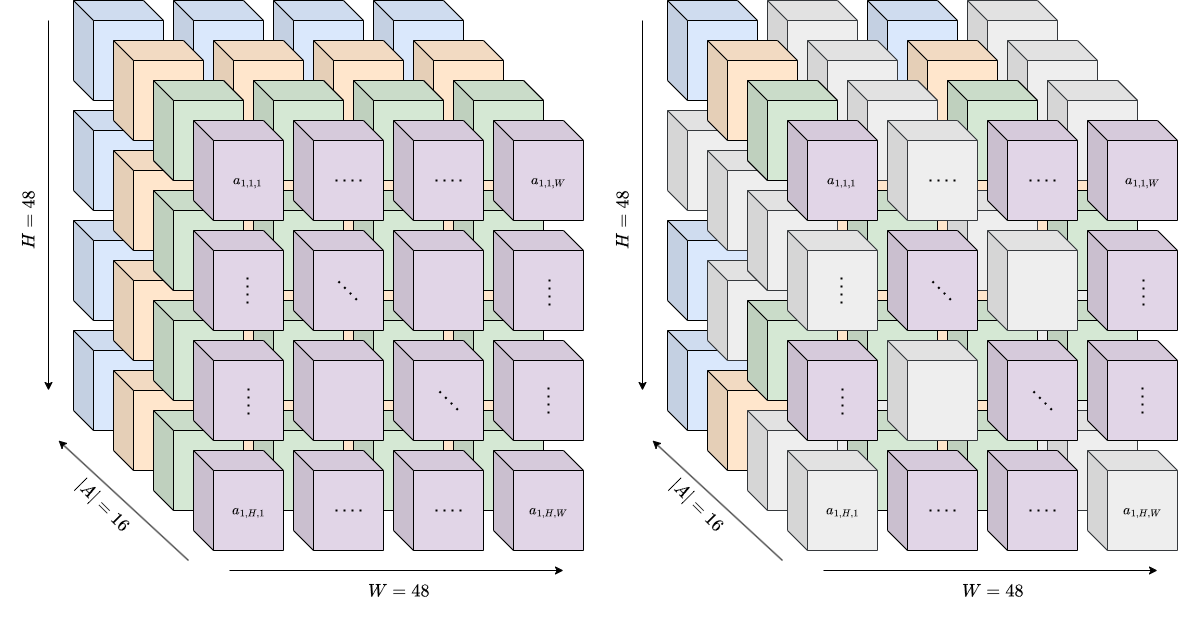
\includegraphics[width=0.7\linewidth]{images/methods_mono/action/action_space.png}
    \captionsetup{justification=justified, singlelinecheck=false, width=1\linewidth, labelfont=bf} 
    \caption[]{A comprehensive representation of an action tensor is depicted on the left, alongside its masked version utilizing invalid action masking. Here, \textbdd{masked out} refers to actions that are deemed invalid in the environment given a state $s$. Similarly, colored boxes indicate the same actions across different pixels of the environment. This representation has limitations, as it shows each pixel on a $4\times4$ grid with $4$ possible actions each. From the illustration, it is also visible that invalid action masking effectively reduces the exploration space of the environment for the learner agent.}
    \label{fig:action_space_mono}
\end{figure}



\subsection{Observation}
\label{subsec:mono-observation}

\noindent The observation features were also overhauled from the single-unit testbench (\autoref{subsec:single-observation}), aiming to create a compact observation space while still providing the model with all relevant information. These features can be categorized into four groups: \textbdd{global features, map features, unit features, and factory features}. Global features consist of scalar values that are tiled to the shape of the map for concatenation with other features. Map, unit, and factory features are all shaped \textbdd{H x W}, where \textbdd{H} represents the game board's height and \textbdd{W} its width, describing the tile of the board, units, and factories respectively. Features are represented as 32-bit floating-point numbers. Boolean flags are converted to zeros and ones, while other values are normalized to a \textbdd{[-1, 1] range}. This normalization ensures that the mean of the inputs are close to zero, aiding convergence (\cite{Normalization}). All features are concatenated as channels into a single tensor within the model. See \autoref{tab:features} for a complete list of features.

\bigskip

\noindent The model additionally receives two matrices, each cell containing the ID of the unit or factory occupying that position on the map, representing the entity's team affiliation. These matrices do not alter entity behavior but are utilized during training for reward assignment, critic values, log probabilities, and entropy values. Further details on reward assignment will be provided in \autoref{subsec:grouping}.

\begin{table}[htbp]
    \centering
    \begin{tabular}{|c|c|c|c|}
        \hline
        \textbf{Feature Type} & \textbf{Feature Name} & \textbf{Shape} & \textbf{Value Range} \\
        \hline
        Global & Step & Scalar & [-1, 1] \\
        Global & Daytime & Scalar & \{0, 1\} \\
        \hline
        Map & Friendly Factory & H x W & \{0, 1\} \\
        Map & Ice & H x W & \{0, 1\} \\
        Map & Ore & H x W & \{0, 1\} \\
        Map & Rubble & H x W & [-1, 1] \\
        Map & Friendly Unit & H x W & \{0, 1\} \\
        Map & Enemy Unit or Factory & H x W & \{0, 1\} \\
        \hline
        Unit & Heavy Unit & H x W & \{0, 1\} \\
        Unit & Power in Battery & H x W & [-1, 1] \\
        Unit & Ice in Cargo & H x W & [-1, 1] \\
        Unit & Ore in Cargo & H x W & [-1, 1] \\
        \hline
        Factory & Power in Factory & H x W & [-1, 1] \\
        Factory & Ice in Factory & H x W & [-1, 1] \\
        Factory & Water in Factory & H x W & [-1, 1] \\
        Factory & Ore in Factory & H x W & [-1, 1] \\
        Factory & Metal in Factory & H x W & [-1, 1] \\
        \hline
    \end{tabular}
    \captionsetup{justification=justified, singlelinecheck=false, width=1\linewidth, labelfont=bf}
    \caption{Table containing the complete list of observation features, along with their shape and normalized value range. $H$ and $W$ refer to the height and width of the board.}
    \label{tab:features}
\end{table}

\subsection{Weight Scaling}
\label{subsec:weight-scaling}

\noindent The scaling factor of the weight initialization can have a substantial effect on the \textbdd{variance} of both the \textbdd{activations and the gradients} (\cite{pmlr-v9-glorot10a}). Proper weight initialization for the Rectified Linear Unit (ReLU) activation function with the scale of $\sqrt{\frac{2}{n_t}}$, where $n_t$ is the number of input units to the layer, has been shown to ensure \textbdd{zero mean and unit variance} of the outputs (\cite{DBLP:journals/corr/HeZR015}), stabilizing the learning process. Omitting the $n_t$ terms causes higher variance but has been widely used in practice, for which the original PPO implementation is a good example. Since we use Leaky ReLU activations, we employed the slightly modified scaling of \autoref{eq:gain}, which was the scaling recommendation for that specific activation in the Pytorch framework (\cite{pytorchinit}).

\begin{equation}
    \texttt{gain} = \sqrt{\frac{2}{1+\texttt{negative\_slope}^2}}
\label{eq:gain}
\end{equation}

\bigskip

\noindent Following the recommendations of \cite{shengyi2022the37implementation}, we used the activation function's recommended gain value as the scale for weight initialization in our hidden layers and a scale of 0.01 for the initialization of the actor head. We initialized the critic with the same scale to get \textbdd{predictions close to zero}, matching our scaled-down rewards (\autoref{subsec:hyb-rew}). After learning how much \textbdd{downscaling the weights} can help, in some benchmark tests boosting performance by 66\% (\cite{andrychowicz2020matters}), we further scaled down the output layers of the network by a factor of 100 to make the action distribution more closely resemble a \textbdd{uniform distribution}. We were still noticing fluctuations in performance based purely on the seed the networks were initialized with, so we performed the same scaling on the critic value output layer's weights and, eventually, the hidden layers.

\subsection{Feature Extractor Model}
\label{sec:monolithic-network}

\noindent We transitioned from a heavily shaped feature space to a \textbdd{CNN-based feature extractor}, aiming to map the observations detailed in section (\autoref{subsec:single-observation}) to an action tensor of size $[16, 48, 48]$. In this representation, 16 signifies the size of the discrete action space, while 48 denotes the map size. Given that both our observation tensor and action space possessed a channel size of 16, encompassing various map, unit, factory, and global features (\autoref{tab:features}), we required a mapping strategy to align the observation space with the action space structure (\autoref{sec:monolithic-network}). We implemented two distinct feature extractor architectures to achieve this goal.

\bigskip

\noindent The first network architecture adopted a U-Net style encoder (\cite{ronneberger2015unet}) with various variations of bottlenecks and a decoder with skip connections (\cite{wu2020skip}). U-Net architectures are well-known for their effectiveness in image segmentation tasks (\cite{ehab2023performance}; \cite{ronneberger2015unet}), and we aimed to achieve a similar outcome but at the \textbdd{entity level segmentation}. Our goal was for the network to recognize that entity-free spaces represented inactive segments of the input space, while units and factories remained segmented as distinct entities. Each entity's class corresponded to the action it performed in the environment. In simpler terms, we aimed to create a segmentation map that \textbdd{established a class system} for each agent, categorizing them into different classes. For instance, if the network predicted a dig action for a unit at a given pixel, it meant that the network had segmented it into a \textbdd{digger} class. Similarly, when the model predicted a recharge action, the corresponding agent was categorized into a \textbdd{recharger} class within the grid environment.

\bigskip

\noindent The encoder of the network employed \textbdd{Downsampling blocks}, transforming the input tensor from a shape of $[16, 48, 48]$ to $[256,3,3]$. Each Downsampling block comprised a residual block (\autoref{subsec:residual}) and a downsampling convolutional layer with a kernel size of 3 and a stride of 2, effectively \textbdd{halving} the height and width of its input. The residual blocks consisted of 2 convolutional layers, a squeeze-and-excitation layer (\autoref{subsec:se}), and a leaky ReLU (\autoref{subsec:leaky-relu}) as the residual, which was concatenated to the input of the residual block. Spectral (\autoref{subsec:spectralnorm}) and batch normalization (\autoref{subsec:batchnorm}) techniques were applied after each convolutional layer, followed by a leaky ReLU activation function.

\bigskip

\noindent Furthermore, each convolutional layer was initialized using orthogonal initialization techniques (\autoref{subsec:ortho}) following recommendations from the literature (\cite{shengyi2022the37implementation}). The weights have been further scaled down to minimize the fluctuations in performance between seeds that random initialization can cause (\autoref{subsec:weight-scaling}). To ensure reproducibility and \textbdd{reduce variation in different trial runs}, each layer was initialized with a combination of the global seed and the layer's unique hash. The Squeeze-and-Excitation module employed a reduction factor of 16, facilitating the calculation of channel weighting and importance for every input channel of the observation feature.

\bigskip

\noindent We explored various bottleneck architectures, including a \textbdd{simple convolutional bottleneck} comprising two residual blocks and and a \textbdd{multi-scale bottleneck} incorporating $1\times1$, $3\times3$, $5\times5$, and $7\times7$ convolution operations to expand the receptive field of the model (\cite{Gao_2021}). The multi-scale U-net architecture, in particular, aims to mitigate degradation issues in target regions of segmentation masks by creating representations of the input on different receptive fields and concatenating them to form a comprehensive feature space representation. This approach has been demonstrated to be effective in maintaining the integrity of target regions in segmentation tasks (\cite{article_bot}; \cite{zhu2024efficient}; \cite{bhojanapalli2020lowrank}). 

\bigskip

\noindent In the decoder component of the network, we designed upsampling blocks that mirrored the structure of the downsampling blocks but in reverse. Each upsampling block begins with a \textbdd{transpose convolution} (\cite{shelhamer2016fully}) to upsample the input feature map, followed by batch and spectral normalization and a leaky ReLU nonlinearity. The block concludes with a residual block, maintaining consistency with the previous structure. The inputs to the upsampling blocks consist of outputs from preceding layers and corresponding residuals from their paired downsampling blocks. We termed this feature extractor network the \textbdd{BottleNet} (\autoref{fig:BottleNet}).

\bigskip

\begin{figure}[htbp]
    \centering
    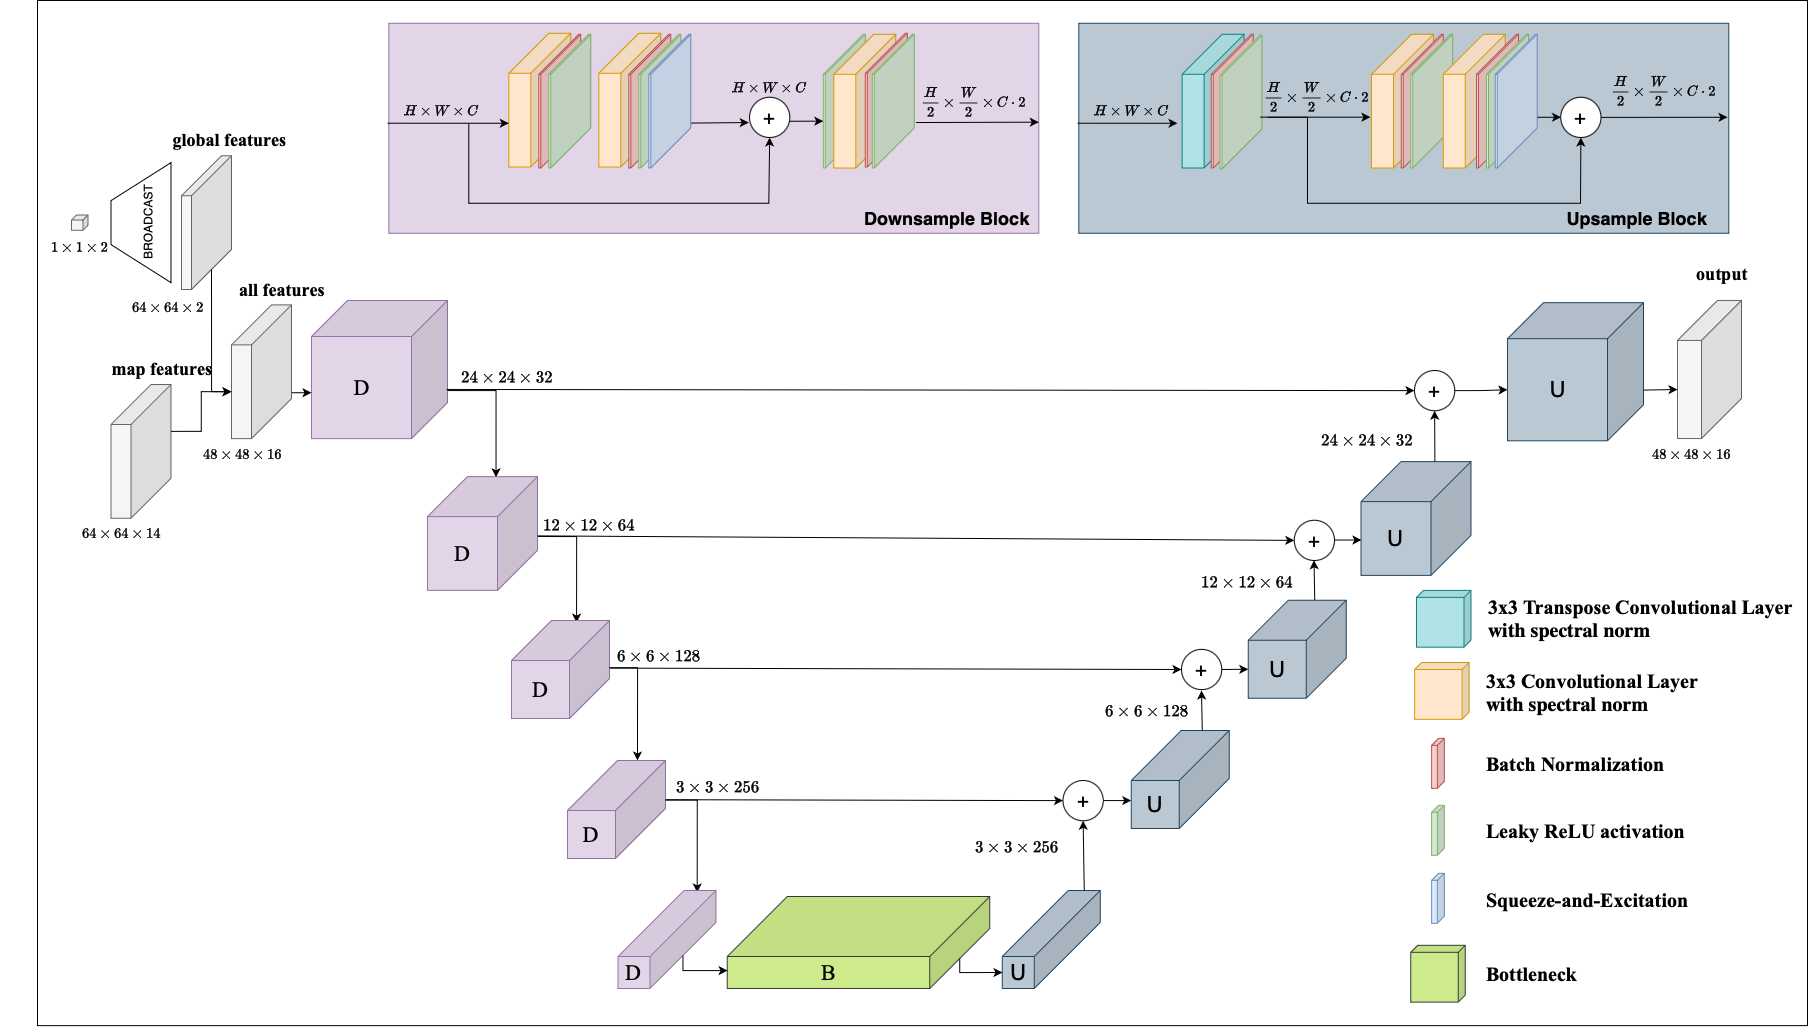
\includegraphics[width=0.9\linewidth]{images/methods_mono/feature_extractor/unet.png}
    \captionsetup{justification=justified, singlelinecheck=false, width=1\linewidth, labelfont=bf} 
    \caption[]{The figure depicts the entire feature extractor network, encompassing the process from input to output. Map features are combined with tiled-up global features, passing through a sequence of Downsample Blocks until reaching the bottleneck layer. The bottleneck layer's outputs are then upsampled via a series of Upsample Blocks, utilizing matching residuals from downsampling blocks to retain information. Finally, the output is directed towards both the critic and actor networks.}
    \label{fig:BottleNet}
\end{figure}

\begin{figure}[htbp]
    \centering
    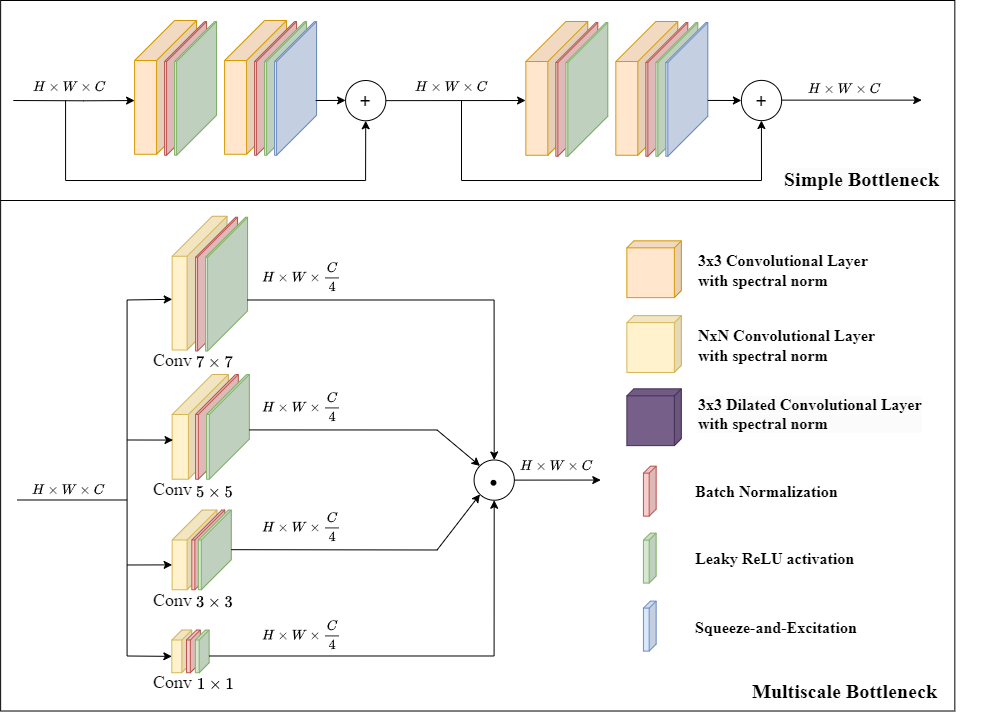
\includegraphics[width=0.8\linewidth]{images/methods_mono/bottleneck/bottleneck.png}
    \captionsetup{justification=justified, singlelinecheck=false, width=1\linewidth, labelfont=bf} 
    \caption[]{The three images illustrate various types of bottlenecks tested for our feature extractor. Starting from the top, the Simple Bottleneck consists of two residual blocks. The Dilated Bottleneck employs convolutional layers with dilation, where the filter expands by a certain factor, allowing it to capture a broader context. Lastly, the Multiscale Bottleneck features a four-branch network, emphasizing important features at different scales.}
    \label{fig:Bottlenecks}
\end{figure}


\noindent For our second network architecture, we opted to maintain the input and output sizes \textbdd{without downscaling}, thus eliminating bottleneck layers. With the goal of creating a one-to-one mapping, we designed a compact residual network that preserves the height and width of the feature maps throughout the network. This network comprises an input convolutional block with spectral normalization, batch normalization, and leaky ReLU nonlinearity. It is followed by four residual blocks, each incorporating SE layers for channel importance weighting, similar to the BottleNet architecture. The final block of this feature extractor network consists of another convolutional block with spectral normalization, batch normalization, and a leaky ReLU activation function. We named this feature extractor the \textbdd{DashNet}.

\subsection{Actor and Critic}
\label{sec:mono-network-actor-critic}

\noindent To ensure compatibility with Stable Baselines, we introduced an additional layer of feature extractor, separated for both the actor and policy networks. To simplify and reduce computational load, we applied a $3\times3$ convolutional layer to the output of our feature extractor network for the actor, incorporating batch, spectral, and layer normalization techniques. Then, for each pixel, its corresponding output value was sent through a linear projection layer, which mapped the extractor network outputs to action \textbdd{loglogits}. For the value network, to fully represent the value of the entire state from the output tensor, we used a single convolutional block paired with layer normalization and leaky ReLU nonlinearity. To refine the representation of value estimates, this mapping compressed the values into a more suitable space, enabling the inclusion of small negative values for more accurate estimates. Next, we employed a \textbdd{global average pooling method} \cite{lin2014network} to average the values of all pixels channel-wise, resulting in a 48x48-sized tensor. This tensor was then flattened and passed through a linear projection layer to produce the final value estimate (\autoref{fig:mono-actor-critic}).

\begin{figure}[htbp]
    \centering
    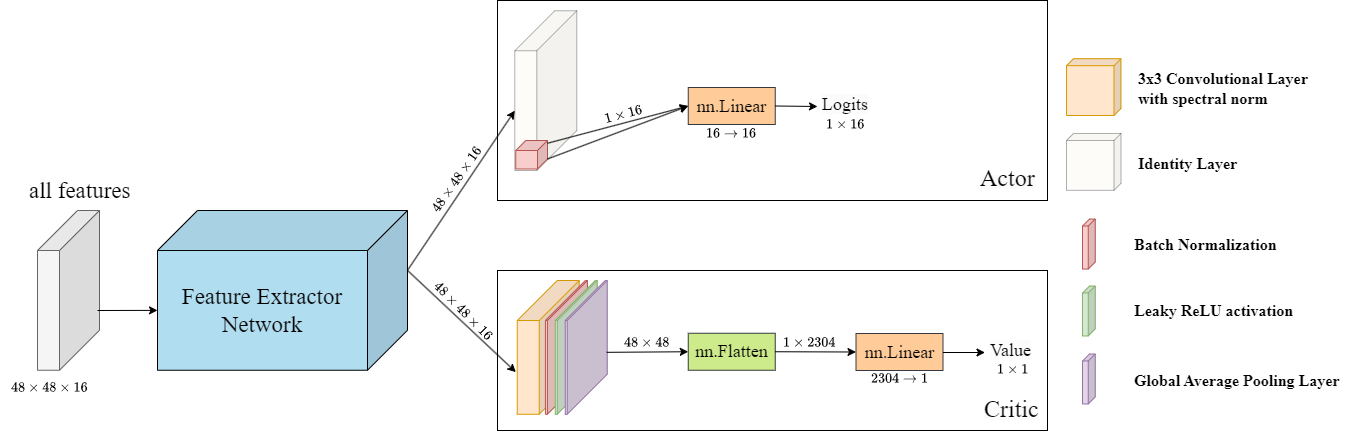
\includegraphics[width=1\linewidth]{images/methods_mono/actor_critic/actor-critic-head.png}
    \captionsetup{justification=justified, singlelinecheck=false, width=1\linewidth, labelfont=bf} 
    \caption[]{The diagram shows the actor and critic heads of the architecture. The actor head extracts action vectors for each pixel using an identity layer and a linear projection for logits. Meanwhile, the value head utilizes a final convolutional block with Global Average Pooling to calculate channel-wise averages, followed by a many-to-one linear projection.}
    \label{fig:mono-actor-critic}
\end{figure}

\subsection{Reward Function}
\label{sec:monolithic-reward-function}

\noindent We adjusted the rewards to incentivize global \textbdd{ice collection, ice transfer, and water generation} in the environment. Ice collection was scaled down by a factor of four to normalize its value to that of water (as 4 ice can be turned into 1 water by the factory). Additionally, we further downscaled the ice collection by a tenth to incentivize not only the digging of ice but also its transfer to factories, which was rewarded 10 times more than simple collection. Water production was rewarded by a single unit, as it is the key metric for sustaining the factory and aligning our model with the task of maintaining factory viability. In order to incentivize units to fill the factories with ice as early as possible, the rewards are \textbdd{multiplied by a factor}, made by the following function:

\begin{equation}
    f(\texttt{step}) = 1 + (1000 - \texttt{step}) / 1000 \times 0.1
    \label{eq:reward-early-scaling}
\end{equation}

\noindent This factor \textbdd{boosts the rewards} more the closer we are to the \textbdd{start of the episode}. Our final reward function is the following: 

\begin{align}
    r(\texttt{step}) = \frac{0.01}{f(\texttt{step})} \left[ 
    \frac{\Delta \texttt{ice\_dug}}{40} 
    + \frac{\Delta \texttt{ice\_transferred}}{4} 
    + \Delta \texttt{water\_produced}
    \right]
    \label{eq:reward-mono}
\end{align}

\subsection{Training}
\label{sec:monolithic-approach-training}

\noindent We maintained the training environment and learning algorithm consistent with the single-agent testbench (\autoref{sec:single-unit-testbench}), employing Stable Baselines and its maskable PPO variant (\autoref{subsec:M-PPO}). While Stable Baselines is known for its compatibility with various single-agent environments (\cite{stable-baselines3}), it required significant adaptation for environments where a central decision maker governs actions for multiple entities. Consequently, we underwent a \textbdd{complete rewrite of the PPO learning algorithm} from Stable Baselines to align with our requirements.

\bigskip

\noindent Our action space underwent a transformation from a single discrete 1x12 tensor to a \textbdd{multidiscrete} 16x48x48 tensor. Within each HxW dimension, a 16-dimensional log logit tensor was generated. After exponentiation, an action mask was created for all logits in all HxW dimensions, effectively reducing the corresponding masked values to extremely small numbers, resulting in near-zero probabilities during normalization. Consequently, we had to permute and correctly reshape the action mask and policy head values to tensors of shape 48x48x16. Subsequently, for the calculation of log probabilities, advantages, entropy, and actions, a 48x48 tensor had to be supplied. While further refinements and adjustments were made, detailed discussions on these intricate aspects are omitted here, as they are available in our publicly accessible repository (\url{https://github.com/MagmaMultiAgent}).

\bigskip

\noindent It's crucial to note that implementing self-play in a multi-entity environment using stable baselines is not straightforward (\cite{stable-baselines-issue181}). As a workaround, we employed a passive enemy agent that doesn't interact with the environment. Consequently, our M-PPO algorithm could only learn from the experiences collected by one player, effectively halving the available training data. To compensate for this reduction, we \textbdd{doubled the size of the rollouts} from 4,096 to 8,192. Additionally, to maintain the desired number of updates during batched gradient descent at 8, we set the minibatch size to 1,024. For a comprehensive overview of the hyperparameters and environment settings, please refer to \autoref{app:b}. 

\bigskip

\noindent We originally chose to train the agent over 102,400 steps, corresponding to 25 evaluation phases, with each phase covering rollouts of size 4,096 steps. However, since self-play was not implemented in Stable Baselines (\cite{stable-baselines-issue181}), we extended the training to 204,800 steps ($8,096 \times 25$) to compensate. This ensured that we \textbdd{maintained the same number of model updates} (25), approximating a self-play environment as closely as possible.

\subsection{Evaluation}
\label{sec:monolithic-approach-eval}

\noindent We standardized our evaluation phases by conducting \textbdd{evaluations after every training phase}, totaling 8,192 steps, using 12 environments with an extended episode length of 1,000, the upper limit in the Lux AI Competition (\autoref{sec:environment}). We employed different seeds for the evaluation environments to thoroughly assess the model's generalization performance. Logging global metrics, including overall ice dug, transferred, and water generated in each evaluation environment, we conducted three trials as before for the single-unit test bench. For the final result, we averaged the global metrics collected for every parallel environment per trial ($3\times12$ environments) and calculated their standard deviation. It's worth noting that not all environments ran for the same number of steps; in such cases, we computed averages and deviations based on the longest step environment and \textbdd{filled any gaps with zeros} where the \textbdd{environment ended sooner}. As for convergence, we measured the agent's ability to keep at least one factory alive until the end of the standard episode length of 1,000 steps in the Lux AI Competition.

\section{Hybrid Approach}
\label{sec:hybrid-approach}

\noindent In order to overcome the difficulties of both the monolithic architecture (\autoref{sec:monolithic-approach}) and fully multi-agent methods, we implement a \textbdd{pixel-to-pixel} architecture \label{par:pixel-to-pixel} (\cite{chen2023emergent}) for our hybrid \textbdd{centralized control} model. Just like in the monolithic architecture, the global observation is fed into a convolutional neural network, which outputs an \textbdd{action for every pixel of the board}. The actions of factories and units are obtained by selecting the resulting action at their corresponding position. The main difference comes in the shape of the network. The pixel-to-pixel architecture preserves the board's shape at all steps, allowing the model to \textbdd{learn simple mappings} instead of relying on a bottleneck to interpret game state. These mappings can be further simplified by the use of residual connections (\autoref{subsec:residual}). By keeping the shape of the layer outputs consistent, we can allow each action output to be based on features in the corresponding \textbdd{entity's neighborhood}. Global information can also be accessed by using repeated convolution operations, as shown in \autoref{fig:field_of_view}. Generating all actions for each pixel from a single global observation is very similar to \textbdd{processing batched local observations} for \textbdd{multiple entities separately}. An example can be seen on \autoref{fig:map}. The pixel-to-pixel approach is \textbdd{computationally faster} and requires less data to be stored in memory. Moreover, by using a shared convolutional network, the entities can access each other's internal representations of the game state, establishing a possible \textbdd{channel for communication} (\cite{pmlr-v97-han19a}).

\begin{figure}[htbp]
    \centering
    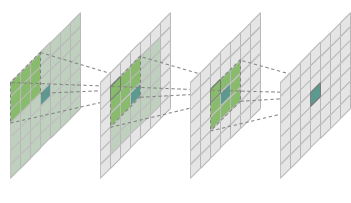
\includegraphics[width=0.7\linewidth]{images/methods_hybrid/field_of_view.png}
    \captionsetup{justification=justified, singlelinecheck=false, width=1\linewidth, labelfont=bf} 
    \caption[]{Figure demonstrating how the use of repeated convolution operations can process global information. The center of the 7x7 grid is marked with ocean color, and it represents an entity in the Lux environment. The increasing field of view is indicated by the shaded green area. The image shows how both local and global information can be utilized in the generation of the entity's action.}
    \label{fig:field_of_view}
\end{figure}

\begin{figure}[htbp]
    \centering
    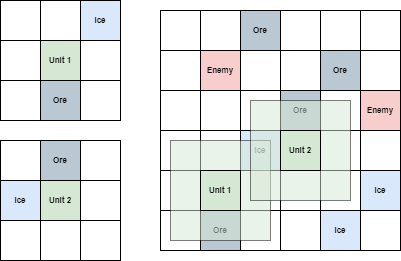
\includegraphics[width=0.7\linewidth]{images/methods_hybrid/feature_extractor/map.png}
    \captionsetup{justification=justified, singlelinecheck=false, width=1\linewidth, labelfont=bf} 
    \caption[]{Figure showing how performing shape-preserving convolution operations on the whole observed map (right) is similar to having localized observations for every unit (left). The image represents a segment of the observed game board. The range of a 3x3 convolution around the units can be seen on the right, marked by an opaque green filter.}
    \label{fig:map}
\end{figure}

\bigskip

\noindent Because a central decision maker is used, but in a way that allows each agent to make their decisions based on their \textbdd{localized observations}, similarly to a distributed method, we call this approach \textbdd{hybrid}. Later, we augment this method with the ability to \textbdd{assign rewards to individual} factories and units instead of purely global rewards. This change makes our approach more similar to a truly multi-agent control system while maintaining the benefits of operating with a \textbdd{single global observation} of the game board. We will compare this modified reward-assignment method to the original global reward system. For a more detailed comparison of the mentioned methods, please refer to \autoref{tab:hybrid-table}.

\bigskip

\noindent The training goal remained consistent for this phase as well: \textbdd{learn how to keep factories alive} until the end of the episode. We will now outline the specifications of the training algorithm and model used in the test.

\begin{table}[htbp]
    \centering
    \begin{tabularx}{\linewidth}{|Y|C{2.3cm}|C{2.3cm}|C{2.3cm}|C{2.3cm}|C{2.3cm}|}
        \toprule
        \textbf{Property} & \textbf{Monolithic} & \textbf{Distributed with Local Observations} & \textbf{Distributed with Global Observations} & \textbf{Hybrid with Global Trajectories} & \textbf{Hybrid with Separate Trajectories} \\
        \midrule
        Passes through Model & once & per agent & per agent & once & once \\
        \midrule
        Features Stored & once & per agent & per agent & once & once \\
        \midrule
        Stored Feature Size & global & local & global & global & global \\
        \midrule
        Field of View & global & local & global and local & global and local & global and local \\
        \midrule
        Distributed Rewards & no & yes & yes & no & yes \\
        \midrule
        Handles Changing Agent Numbers & yes & no & no & yes & yes \\
        \bottomrule
    \end{tabularx}
    \captionsetup{justification=justified, singlelinecheck=false, width=1\linewidth, labelfont=bf} 
    \caption{Table showing the differences between agent control architectures. While storing global observations for every agent with a distributed approach is similar to the hybrid architecture, it requires much more memory and cannot handle changing agent numbers. A hybrid architecture with separating trajectories (\autoref{subsec:grouping}) has every benefit of distributed control.}
    \label{tab:hybrid-table}
\end{table}

\subsection{Environment}

\noindent The environment largely aligns with the description in \autoref{subsec:mono-environment}, with notable changes made to the action space. It now encompasses \textbdd{all actions available} in the Lux AI environment (\autoref{subsec:lux-action}), with a few exceptions, detailed in \autoref{subsec:actions}. Additionally, a \textbdd{stricter action masking} mechanism has been applied to limit unnecessary movements and collisions among units.

\subsection{Heuristic Bidding and Factory Placement}

\noindent We retained our initial Gaussian factory placement heuristic outlined in \autoref{subsec:heur-bidding-factory}, making minor adjustments to the weighting calculation and scale of the Gaussian filters to ensure factories are positioned \textbdd{as close as possible to ice}.


\subsection{Actions} \label{subsec:actions}

\noindent Since our goal is to keep the factories alive until the end of the game, we decided to \textbdd{get rid of the lichen mechanic} completely via action masking. This meant that the factories had three possible actions left: build heavy, build light, and do nothing. We forbade the self-destruct action for units since hostility was not needed to achieve the simplified objective.

\bigskip

\noindent Unit actions are comprised of an action type and action settings, depending on the type. Most action settings were implemented heuristically, such as the transfer amount and the repeat flag; however, the most significant parameters were left for the model to decide. Parameters include the move direction, pickup amount, transfer direction, and transfer resource.

\bigskip

\noindent We \textbdd{forbade illegal actions}, such as factory actions that require more resources than the factory's current cargo, moving out of the map, and choosing unit actions that need more power than the agent's current battery. Actions that would slow down exploration were also disabled to \textbdd{speed up the training}. Such actions are doing nothing when the factory could be producing heavy units with its resources, units recharging, or picking up power from factories while at full power. Agent collisions between the team members were also disabled, with keeping track of each unit's movement possibilities and allowing only one at a time to step on a board tile. To stop factories from spawning new units on top of existing ones, agent creation is masked out if a unit is standing on the middle tile of a factory. Agents cannot enter the middle of factories once they have stepped away from them. Actions we considered too complex and unnecessary for the game were also removed with masking, such as picking up resources from factories and transferring resources or power to other agents. The complete list of possible actions and their requirements can be found in \autoref{tab:actions}.

\begin{table}[htbp]
    \centering
    \begin{tabular}{p{1.5cm}|p{3cm}|p{3cm}|p{6cm}}
        \hline
        Entity & Action & Parameters & Requirements \\
        \hline
        Factory & Build Heavy unit & None & - 100 metal in factory \newline - 500 power in factory \newline - middle of factory is empty \\
        \hline
        Factory & Build Light unit & None & - 10 metal in factory \newline - 50 power in factory \newline - middle of factory is empty \\
        \hline
        Factory & Do nothing & None & - no resources to build heavy unit \\
        \hline
        Unit & Do nothing & None & - no power to update action queue \\
        \hline
        Unit & Recharge & Amount [0, 10] & - battery not full \\
        \hline
        Unit & Pickup & Amount [0, 10] & - battery not full \newline - standing on factory \\
        \hline
        Unit & Move & Direction [0, 4] & - no friendly unit at target \newline - enough power \newline - no enemy factory at target \\
        \hline
        Unit & Transfer & Direction [0, 5] \newline Resource [0, 1] & - has cargo \newline - target is factory \\
        \hline
        Unit & Dig & None & - standing on ice, ore or rubble \newline - enough power \\
        \hline
    \end{tabular}
    \captionsetup{justification=justified, singlelinecheck=false, width=1\linewidth, labelfont=bf}
    \caption{Table containing the list of possible actions, along with their requirements. If the requirements are not fulfilled, the action is masked out.}
    \label{tab:actions}
\end{table}


\subsection{Observation}

\noindent We maintained the observation space described in \autoref{subsec:mono-observation}, as it already covered the necessary information for the feature extractor model to align agents for ice resource collection and survivability. Although additional \textbdd{location information} was provided to the network, it was only utilized for \textbdd{auxiliary purposes} and filtering, not incorporated into the forward pass of the feature extractor.

\subsection{Trajectory Separation} \label{subsec:grouping}

\noindent In a \textbdd{multi-agent environment}, where the actions of units and factories are deeply intertwined, the question of \textbdd{credit assignment} naturally arises. Suppose we use rewards corresponding to a global objective or to objectives that require the cooperation of multiple units or factories. In such a scenario, tracking whom to reward and what amount is challenging since multiple agents work towards a common goal. A \textbdd{centralized control} approach offers a potential solution, as all units and factories will belong under a single agent, which receives a \textbdd{global reward} after performing the actions with all entities. Such reward assignment is still possible when using a fully multi-agent approach by giving every agent the sum or mean reward of the team. \label{par:global-rew} However, as we will later see, relying purely on global rewards makes it \textbdd{hard for the model to learn} which entity's action was beneficial from the \textbdd{many numbers of entities}. The more entities we have, the \textbdd{less of a chance} there is that most of them \textbdd{behave optimally}. A highly beneficial or detrimental action can skew the total reward, which can lead to the \textbdd{reinforcement of bad behavior} or the \textbdd{punishment of good behavior} for the entities whose reward was less dominant in the final sum.

\bigskip

\noindent To tackle this complex problem, we use rewards that can be \textbdd{immediately credited} to the performing or benefiting entity. The ice-dug reward is credited to the performing unit, while the ice-transfer reward is split between the performing unit and the receiving factory. Instead of summing up these rewards to a single global value, we \textbdd{store them separately} to track which entities' actions resulted in how much reward. Since we are using an actor-critic method for training, the critic values should also be distributed. We utilize separate critic value predictions for each entity (\autoref{sec:hybrid-network-actor-critic}). These separate predictions are generated using information about the whole game state, similar to the method of \cite{lowe2020multiagent}.

\bigskip

\noindent In addition to \textbdd{global} and \textbdd{per-entity} reward assignments, we also experimented with putting entities into \textbdd{groups} according to certain grouping rules, where a group's reward is the sum of its members' reward. An example of the reward separations between different groups can be seen in \autoref{fig:rewards}.

\bigskip

\noindent Similar to the rewards and critic values, we also store the action log probabilities and entropies separately. This separation essentially splits every environment step into \textbdd{multiple training examples}, creating multiple \textbdd{distinct trajectories} from the same number of environment steps. The loss calculation does not change from the original PPO algorithm, as the modification simply translates into an additional tensor dimension, and all of the loss samples will get averaged into a single loss value as shown on \autoref{fig:policy-loss}. After the modification, during backpropagation, the \textbdd{weights can be updated more accurately} to reinforce good and diminish bad behavior since the fewer units and factories that belong to one group, the less of a chance a single entity has of \textbdd{skewing their group's reward}, resulting in an inaccurate advantage calculation and a faulty weight update. We will refer to this method as \textbdd{trajectory separation}.

\begin{figure}[htbp]
    \centering
    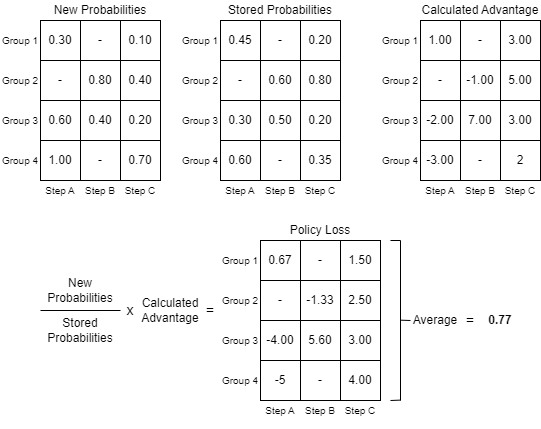
\includegraphics[width=0.7\linewidth]{images/methods_hybrid/trajectory_separation/policy_loss.png}
    \captionsetup{justification=justified, singlelinecheck=false, width=1\linewidth, labelfont=bf} 
    \caption[]{Demonstrating policy loss calculation with the extended dimension. The probabilities and advantages are calculated on a group level. The matrices on the image represent a mini-batch consisting of 3 environment steps. Inactive groups at all steps are marked with a dash, as these are excluded from the training data. The loss gets computed for all active groups, creating more training examples. In the above image, three environment steps resulted in 9 train steps. These loss values are then averaged to get a final scalar loss value. For simplicity, the clipping operation and advantage normalization are left out of this image.}
    \label{fig:policy-loss}
\end{figure}

\begin{figure}[htbp]
    \centering
    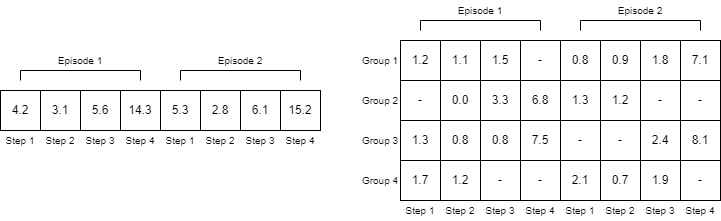
\includegraphics[width=0.8\linewidth]{images/methods_hybrid/trajectory_separation/rewards.png}
    \captionsetup{justification=justified, singlelinecheck=false, width=1\linewidth, labelfont=bf} 
    \caption[]{Image showing the difference between global rewards (left) and rewards distributed into groups (right). The examples are 4-length episodes with random data.}
    \label{fig:rewards}
\end{figure}

\bigskip

\noindent The PPO algorithm uses a \textbdd{termination flag} stored for every step when calculating future rewards during advantage estimation. This flag signals the start of a \textbdd{new episode} and ensures we do \textbdd{not include} this episode's rewards in the \textbdd{cumulative return} calculation of the previous steps. We need to modify this by adding an \textbdd{extra dimension} to the stored termination flag tensor in order to keep track of the lifecycle of every group since we do not want to calculate steps into the cumulative return where the \textbdd{group was inactive}. An example can be seen on \autoref{fig:dones}. A group is marked done when it contains no active units or factories. In the simplest case, when the groups consist of single units and factories, the flag is set to True if the entity: 1. has not been created yet, 2. is destroyed at that step, or 3. remains destroyed. A group consisting of multiple entities can be calculated by performing the \textbdd{AND} operation on each of its member's termination flags. At the first step of an episode, every group is marked done.

\begin{figure}[htbp]
    \centering
    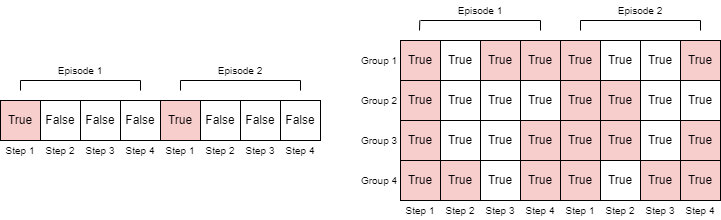
\includegraphics[width=0.8\linewidth]{images/methods_hybrid/trajectory_separation/dones.png}
    \captionsetup{justification=justified, singlelinecheck=false, width=1\linewidth, labelfont=bf} 
    \caption[]{Image showing termination flags for a standard environment (left) and termination flags stored for every group (right). In addition to flagging the end of an episode, the death of a group is also indicated. The examples are 4-length episodes with random data. The cells with true values were given red backgrounds for visibility.}
    \label{fig:dones}
\end{figure}


\noindent If we use a grouping rule that allows groups to be occasionally inactive, for example, by assigning every unit or factory to its own group, the number of training examples belonging to one step will \textbdd{not be constant}. Since we divide the \textbdd{mini-batches} by environment step, this could mean that not all \textbdd{mini-batches} consist of the \textbdd{same number of training examples}. Because the loss values are averaged over a mini-batch to get the final loss, this could mean that training examples that belong to steps with fewer active groups have a \textbdd{more dominant} effect during gradient updates since, on average, they create mini-batches with fewer training examples. Following the same logic, entities at more populated steps of the environment will have \textbdd{less impact} on the final loss. We test using grouping rules that \textbdd{keep group numbers consistent} to overcome this effect. We also experimented with keeping all entity trajectories separate but kept \textbdd{only a set number of training examples} from each step to reduce the training example variance.


\subsection{Feature Extractor Model}
\label{sec:hybrid-network-architecture}

\noindent We use a \textbdd{convolutional neural network} to map the observations into actions for each unit and factory on the board and to output critic values and log probabilities used by the training algorithm. Both the \textbdd{Actor} and \textbdd{Critic} networks have the same \textbdd{Embedding Network} but do not share the weights to avoid the competing objectives of the policy and value functions (\cite{shengyi2022the37implementation}). The structure of the embedding can be seen on \autoref{fig:embedding}. The main building blocks of the network are convolutional layers with \textbdd{3x3 kernels} and padding to \textbdd{keep the board's shape}. The layers alternate between a basic convolutional layer and a \textbdd{residual connection} (\autoref{subsec:residual}), where two convolutional layers are followed by a \textbdd{Squeeze-and-Excitation} block (\autoref{subsec:se}). Each convolutional layer's output goes into a two-dimensional \textbdd{batch normalization} block (\autoref{subsec:batchnorm}), then to a \textbdd{Leaky ReLU} (\autoref{subsec:leaky-relu}) activation function. The weights of the convolutional layers are scaled by their \textbdd{spectral norm} (\autoref{subsec:spectralnorm}). We also implemented the same weight downscaling outlined in \autoref{subsec:weight-scaling}.

\begin{figure}[htbp]
    \centering
    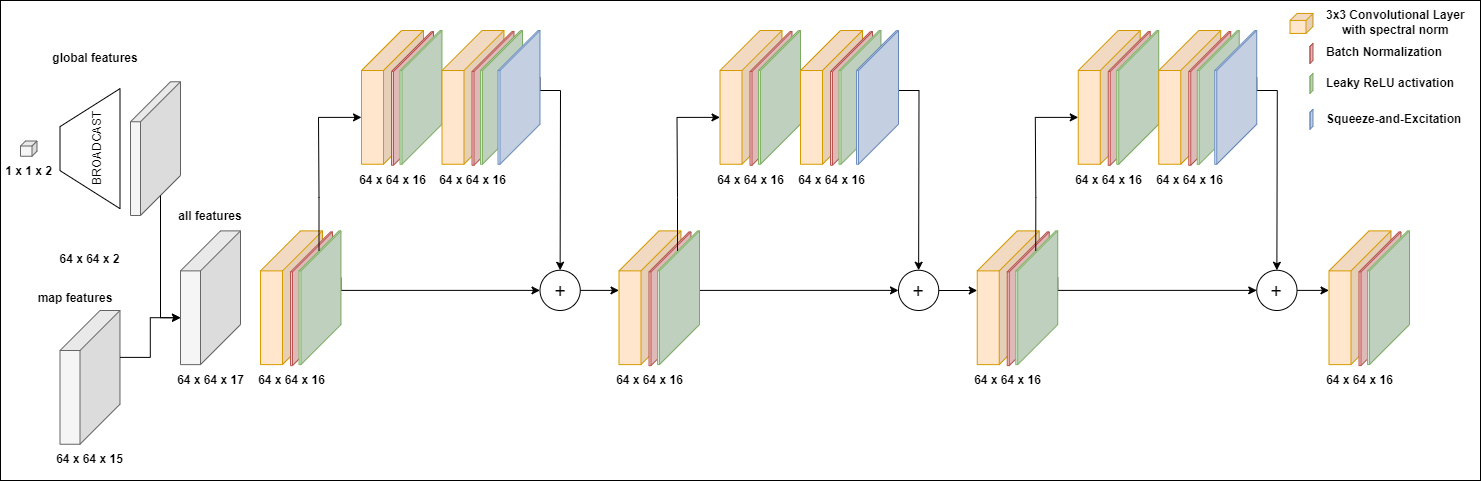
\includegraphics[width=1\linewidth]{images/methods_hybrid/feature_extractor/embedding.png}
    \captionsetup{justification=justified, singlelinecheck=false, width=1\linewidth, labelfont=bf} 
    \caption[]{The structure of the Embedding network. The network uses convolutional layers with 3x3 kernels. Each convolutional block is followed by 2D batch normalization and a Leaky ReLU activation function (\autoref{subsec:leaky-relu}). In order to regularize the network output and allow more layers, we use residual connections with a Squeeze-and-Excitation layer output. This embedding is the backbone of the critic and actor network.}
    \label{fig:embedding}
\end{figure}

\subsection{Actor and Critic}
\label{sec:hybrid-network-actor-critic}

\noindent After the embedding is created from observations, the critic values and the actions are constructed by their respective heads. The Lux environment is highly complex, and the entities need to solve multiple tasks in order to reach their goal. Therefore, multiple reward sources (\autoref{subsec:hyb-rew}) are needed to ensure the rewards are not too sparse for optimal training. In addition to that, since the entities get rewarded based on outcomes, which in reality do not entirely depend on them, it is hard to predict an accurate critic value. Since multiple critic heads already proved to be successful in multi-task environments (\cite{mysore2022multicritic}), we decided to provide a separate critic value prediction for each entity and, in addition to that, provide two additional critic heads for both units and factories, respectively, that use global information for their predictions. The \textbdd{Critic Network} (\autoref{fig:critic}) is made up of 4 components: a \textbdd{unit} and a \textbdd{factory} value network that outputs a value at every board position, and a unit and factory \textbdd{global value} network that, in addition to outputting a value for every position, averages them into a single scalar value. The global unit and factory value scalars are then added to every position of the unit and factory value net output, respectively. This structure ensures that each unit and factory's value calculation is based on \textbdd{both local and global} information. The final output values are created by selecting the predicted value at each unit's and factory's position on the board and then adding the value to the entity's group (\autoref{subsec:grouping}).

\bigskip

\begin{figure}[htbp]
    \centering
    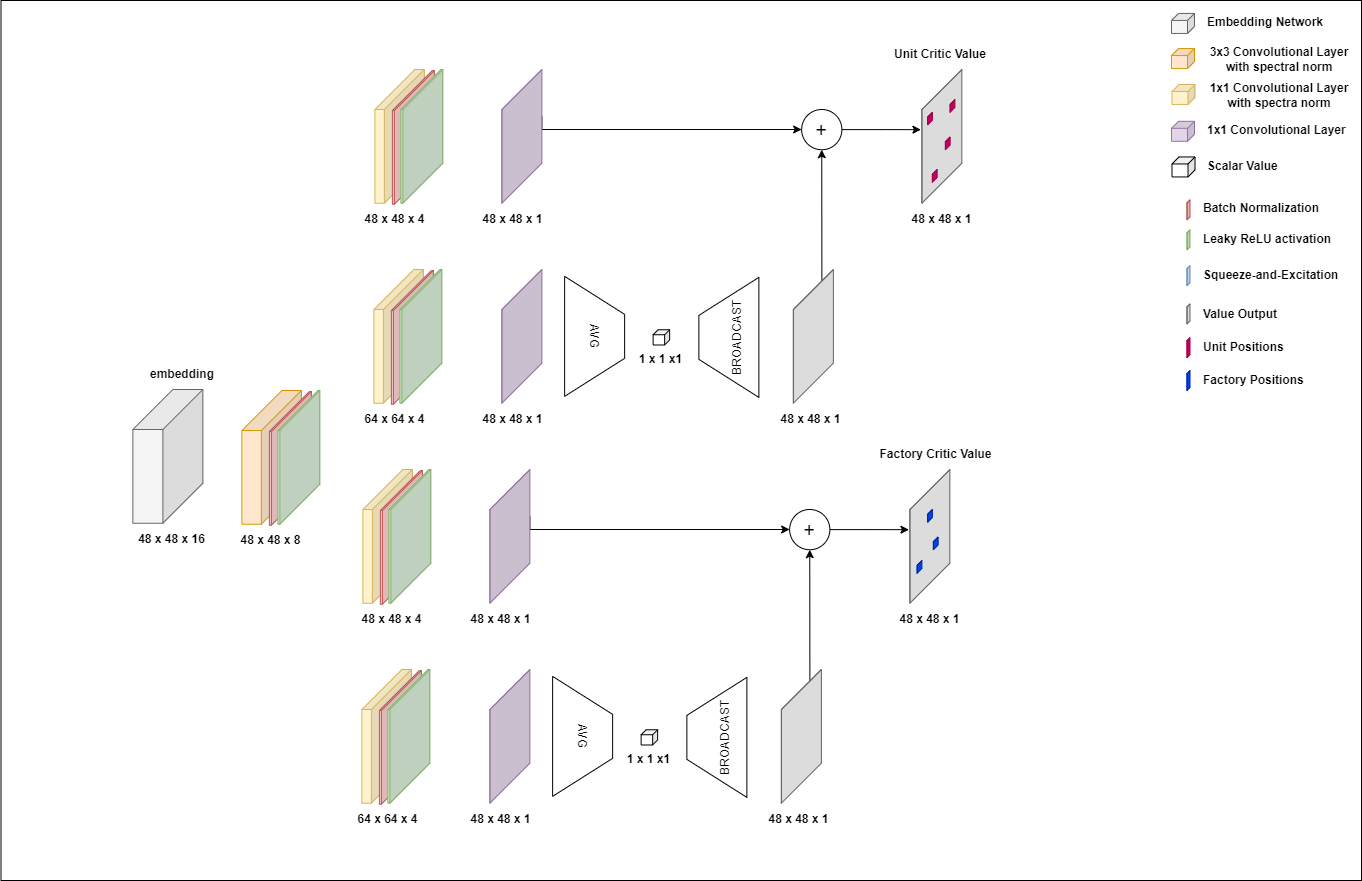
\includegraphics[width=0.9\linewidth]{images/methods_hybrid/actor_critic/critic.png}
    \captionsetup{justification=justified, singlelinecheck=false, width=1\linewidth, labelfont=bf} 
    \caption[]{The Critic network takes the output of the Embedding and outputs critic values for each entity on the board. Each value is comprised of a local value and a global value, which is averaged over the whole board and then added to each position.}
    \label{fig:critic}
\end{figure}

\noindent Actions are created by the \textbdd{Actor Network} (\autoref{fig:actor}). Factories and units have different action spaces, so different actor heads output their actions. The action space of the factories is a simple discrete action space, while the units have a \textbdd{multi-dimensional action space}, where each action has a different set of parameters. Due to some actions having a \textbdd{heuristic parameterization} (\autoref{subsec:actions}), only four parameter action heads are used in addition to the action type head. The heads output log probabilities, which are then used to create \textbdd{categorical distributions} (\cite{categorical}), discrete probability distributions over the possible actions. Actions are sampled from these distributions after setting the probability of masked-out actions to zero. The sampled actions are outputted in the same board shape at the positions of units and factories. For each entity, the composite action's log probability and the distributions' entropies are summed together at an entity level. These values are added to the total log probability and entropy of the given entity's group (\autoref{subsec:grouping}).

\begin{figure}[htbp]
    \centering
    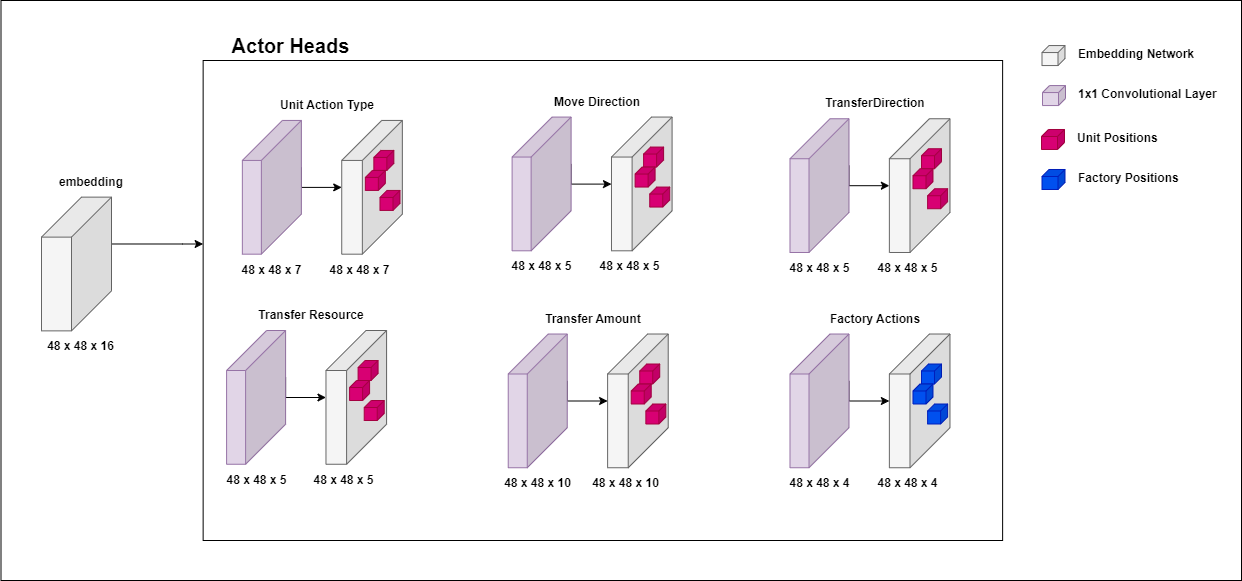
\includegraphics[width=1\linewidth]{images/methods_hybrid/actor_critic/actor.png}
    \captionsetup{justification=justified, singlelinecheck=false, width=1\linewidth, labelfont=bf} 
    \caption[]{The Actor network is made up of separate actor heads, which share the same Embedding network. The output of these heads is the log probabilities of the action distributions. Factory actions have only one output, while unit actions require multiple outputs to parameterize them.}
    \label{fig:actor}
\end{figure}

\subsection{Reward Function}
\label{subsec:hyb-rew}

\noindent The rewards are shaped to \textbdd{encourage the units to bring ice to factories}. In order to achieve this, 1 unit of reward is given after every one water worth of \textbdd{ice is transferred to a factory}. After \textbdd{mining} one water worth of \textbdd{ice}, a $\frac{1}{10}$ unit of reward is given to ensure that units find desirable behavior patterns as early as possible. All of these rewards are then divided by to \textbdd{scale them closer to zero}. In order to incentivize units to fill the factories with ice as early as possible, we utilized the same formulation for the multiplication factor in \autoref{eq:reward-early-scaling}.

\subsection{Training}

\noindent To minimize training duration, we continued utilizing the Masked PPO algorithm (\autoref{subsec:M-PPO}). Our implementation, derived from \cite{luxai_s2-baseline-source}, provided by the contest organizers as a baseline, \textbdd{differes from conventional approaches}. We opted to train the model twice after each rollout step, using data collected from each player separately. This approach enabled us to gather experience from both players without mixing their training examples during mini-batch creation. Leveraging \textbdd{self-play} and access to both enemy and own player data, we halved our rollout size compared to the monolithic approach (\autoref{sec:monolithic-approach-training}) to 4,096 steps. Additionally, we reduced the batch size by a factor of 4, from 1,024 to 256 steps so that we could parallelize more environments. Further details on hyperparameters and subsequent modifications can be found in \autoref{app:c}.

\subsection{Evaluation} \label{sec:hybrid-metrics}

\noindent The evaluation settings remained consistent with those outlined in the monolithic approach (\autoref{sec:monolithic-approach-eval}), except employing 12 evaluation environments. The episode lengths was set to the maximum value of 1,000 steps. While episode length serves as a primary metric reflecting our training goal, measuring the \textbdd{amount of ice transferred by units to factories} provides a more nuanced comparison, as it is practically unbounded, unlike episode length, which can be quickly reached in multiple trials. Additionally, we recorded other metrics, such as the \textbdd{average factory count per step}, to assess the ability of entities to maintain multiple functioning factories instead of just one. Most other metrics were retained as baselines for comparison.

\cleardoublepage

\chapter{Results}
\label{ch:resu}

\noindent This section presents the quantitative results of our experiments with the methods introduced in \autoref{sec:single-unit-testbench}, \autoref{sec:monolithic-approach}, and \autoref{sec:hybrid-approach}. Here's an outline of our result presentation:

\begin{itemize}

\item In \autoref{sec:single-unit-testbench-results} we present results from the single-agent testbench, utilizing metrics such as \textbdd{episode length}, which represents the survival duration of at least one factory of the learning agent, \textbdd{ice dug}, indicating the amount of ice collected by the unit, and \textbdd{ice transferred}, indicating the amount of dug resource given to the factory. The performance of the algorithms is assessed over 1 million steps, resulting in 125 evaluation phases, each comprising 10 updates, totaling 1,250 model updates. The batch size used is 1,024 over rollouts of size 8,192.

\item In \autoref{sec:monolithic-approach-results} we present results from the monolithic network outlined earlier. We use similar metrics as in the single-unit testbench, but introducing the \textbdd{limitation of training episode lengths from 1,024 to 256} to introduce higher \textbdd{quality data} in our rollout buffers. We also reduced the total training steps from 1 million to 104,200, thus achieving 13 rollout phases, 10 epochs each, achieving 130 model updates with the same batch sizes. We also evaluated our top performer model over 1 million steps to assess its convergence capabilities, meaning keeping alive at least one factory for 1,000 steps (\autoref{fig:mono-dash-1M}).

\item In \autoref{sec:hybrid-approach-results} we showcase the novelty of our research: the results on the hybrid agent control. This approach incorporates trajectory separation, distributed credit assignment, multiple actor and value heads, and a highly scalable feature extractor. We introduce a new metric called \textbdd{average factory alive}, indicating not only the agent's capability to keep one factory alive but multiple factories. We conduct experiments with \textbdd{different trajectory numbers} (\autoref{subsec:modulus-grouping}), including \textbdd{top $N$ unit trajectories}, \textbdd{trajectory groupings} (\autoref{subsec:trajec_reduc}), and \textbdd{interchanging separate trajectories with global rewards and advantages} (\autoref{subsubsec:rewardass}). Additionally, we \textbdd{compare our methods with other works} (\autoref{subsec:comparison}) and present a comprehensive \textbdd{ablation study} (\autoref{subsec:ablation}).

\end{itemize}

\section{Single Unit Testbench}
\label{sec:single-unit-testbench-results}

\noindent For our initial comparison, we focused on environment-related metrics such as \textbdd{episode length}, \textbdd{ice dug}, and \textbdd{ice transferred} by units to determine which algorithm performed best in exploration and resource collection tasks. It's important to note that the results presented in \textcolor{deepblue}{\autoref{tab:single-agent-result-env}} are averages from the best-performing evaluation phase out of $125$ evaluation phases, each consisting of 12 environments.

\bigskip

\begin{table}[htbp]
    \centering
    \begin{tabular}{|c|c|c|c|c|c|}
        \hline
        \textbf{Algorithm Type} & \textbf{Algorithm} & \textbf{Episode Length} & \textbf{Ice Dug} & \textbf{Ice Transferred}\\
        \hline
        \multirow{5}{*}{Policy Gradient Methods} & TRPO  & 582  &  4504  & 4320 \\
        \cline{2-5}
         & A2C & 154 &  136  &  62\\
        \cline{2-5}
         & PPO & 473  & 6814  & 6600 \\
        \cline{2-5}
         & R-P\textbf{}PO  & 612 & 6325  & 5892\\
        \cline{2-5}
         & \textbf{M-PPO}  & \textbf{930} &  \textbf{12780} &  \textbf{12340}\\
        \hline
        \multirow{2}{*}{Value-Based Methods} & DQN & 200  & 256  &  204\\
        \cline{2-5}
         & QR-DQN & 690  &  8112 &  8004 \\
        \hline
        Evolutionary Method & ARS & 154 &  0 &  0\\
        \hline
    \end{tabular}
    \captionsetup{justification=justified, singlelinecheck=false, width=1\linewidth, labelfont=bf} 
    \caption{The table presents environment-related results from the single-unit testbench, emphasizing the top performer among all algorithms. \textbdd{M-PPO emerged as the standout performer} among policy gradient methods (\autoref{sec:Policy-Gradient-Methods}), showcasing superior performance attributed to its action masking method. Additionally, R-PPO demonstrated improved performance over standard PPO due to its recurrent nature. Surprisingly, the second-best performing algorithm was a value-based method (\autoref{subsec:value-based-methods}), \textbdd{QR-DQN}, which achieved an average episode length of 690 during its best evaluation phase. QR-DQN also exhibited significant enhancements compared to its standard variation without quantization techniques.}
    \label{tab:single-agent-result-env}
\end{table}

\begin{figure}[htbp]
    \centering
        \centering
        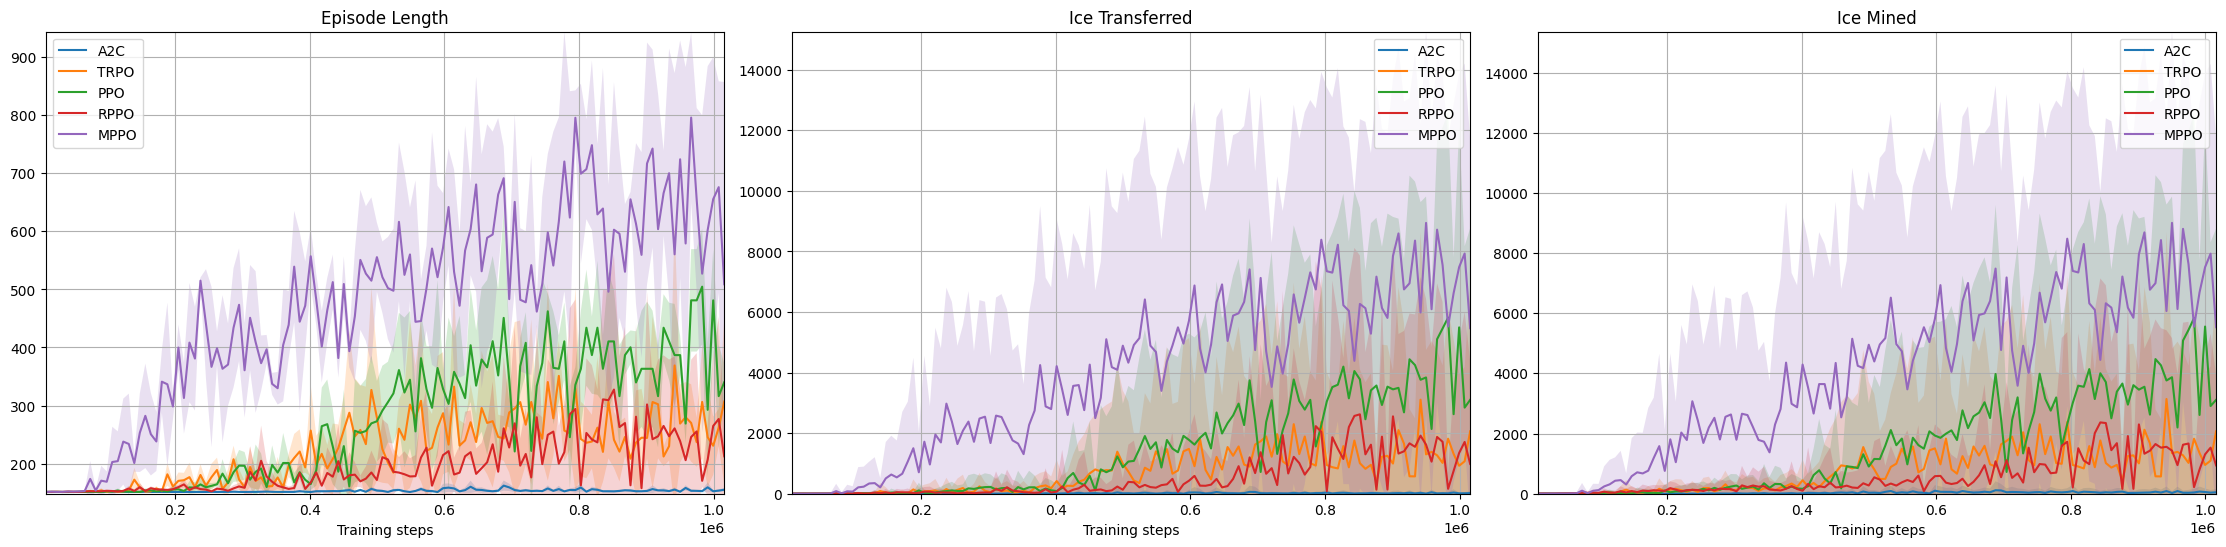
\includegraphics[width=\linewidth]{images/results_singleunit/policy_gradient_single_unit.png}
        \captionsetup{justification=justified, singlelinecheck=false, width=1\linewidth, labelfont=bf} 
        \caption{The three plots depict averages from all three trials of all policy gradient methods alongside their respective evaluation phases, illustrating the average \textbdd{episode lengths}, average \textbdd{ice transferred}, and \textbdd{ice dug}. The data indicates that nearly all policies learned to transfer the collected resource of the unit after digging, as evidenced by the clear similarity between the ice transferred and ice dug plots. Moreover, the images highlight the effectiveness of the invalid action masking technique in M-PPO, which accelerates the learning progress. This is evident from the \textbdd{sharp increase in averages after 204,800 steps}, while maintaining stable updates to the policy.}
        \label{fig:policy_gradient_single_unit}
\end{figure}

\noindent Examining the policy gradient algorithms in \autoref{fig:policy_gradient_single_unit}, we observe that \textbdd{PPO and M-PPO exhibit superior performance} compared to other policy gradient methods in terms of averages. Notably, R-PPO demonstrates higher peaks compared to PPO. Additionally, the plots reveal that certain algorithms, such as \textbdd{A2C, exhibit stagnation with notably low performance}. \textbdd{TRPO} also appears to \textbdd{remain divergent} in a local optimum throughout the evaluations, likely due to its larger updates compared to PPO.

\bigskip

\begin{figure}[htbp]
    \centering
        \centering
        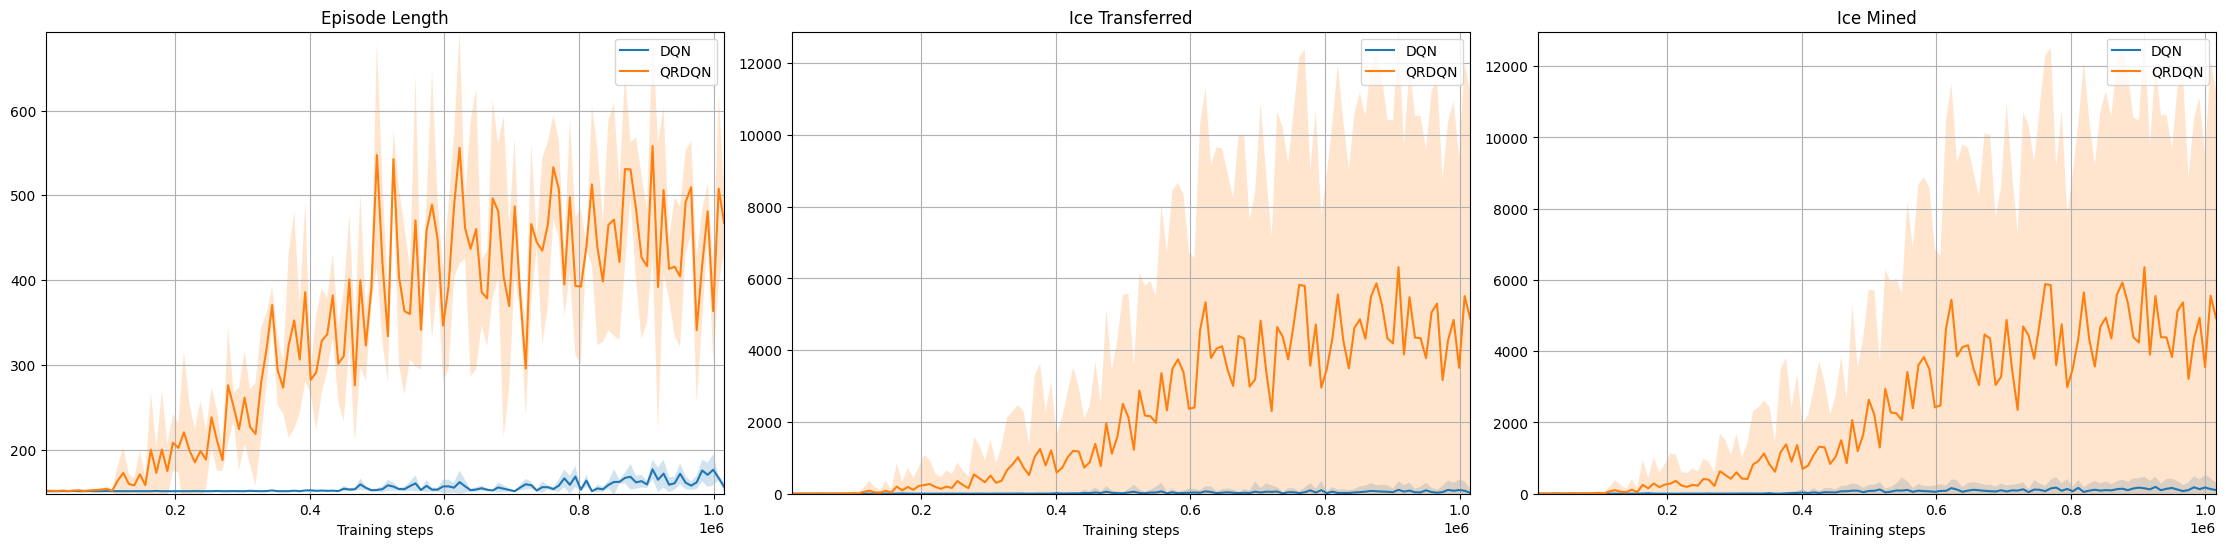
\includegraphics[width=\linewidth]{images/results_singleunit/value_based_single_unit.png}
        \captionsetup{justification=justified, singlelinecheck=false, width=1\linewidth, labelfont=bf} 
        \caption{The three plots display averages from all three trials of all value-based methods, showcasing their performance across various evaluation phases. They illustrate the average \textbdd{episode lengths}, average \textbdd{ice transferred}, and \textbdd{ice dug}. The results highlight a noticeable difference in performance between the two algorithms, with QR-DQN demonstrating significant improvements attributed to its quantization technique.}
        \label{fig:value_based_single_unit}
\end{figure}

\noindent The results depicted in \autoref{fig:value_based_single_unit} clearly \textbdd{favor QR-DQN} for our task. However, it's important to address a significant difference in performance between these two algorithms. QR-DQN utilizes 200 quantiles for its Q value estimates for every state-action pair, leading to a \textbdd{200-fold increase in the output size of the Q-network} compared to its DQN counterpart. This substantial increase in network complexity results in a significant degradation in training performance, with QR-DQN achieving a \textbdd{step-per-second (SPS)} processing speed of 10 compared to DQN's 832. In this context, \textbdd{SPS} refers to the rate at which the algorithm processes steps or actions within the environment per unit of time, measured in seconds. Steps per second were calculated during evaluation phases, including both backward and forward passes during model updates, where a higher SPS indicates better performance.

\begin{figure}[htbp]
    \centering
        \centering
        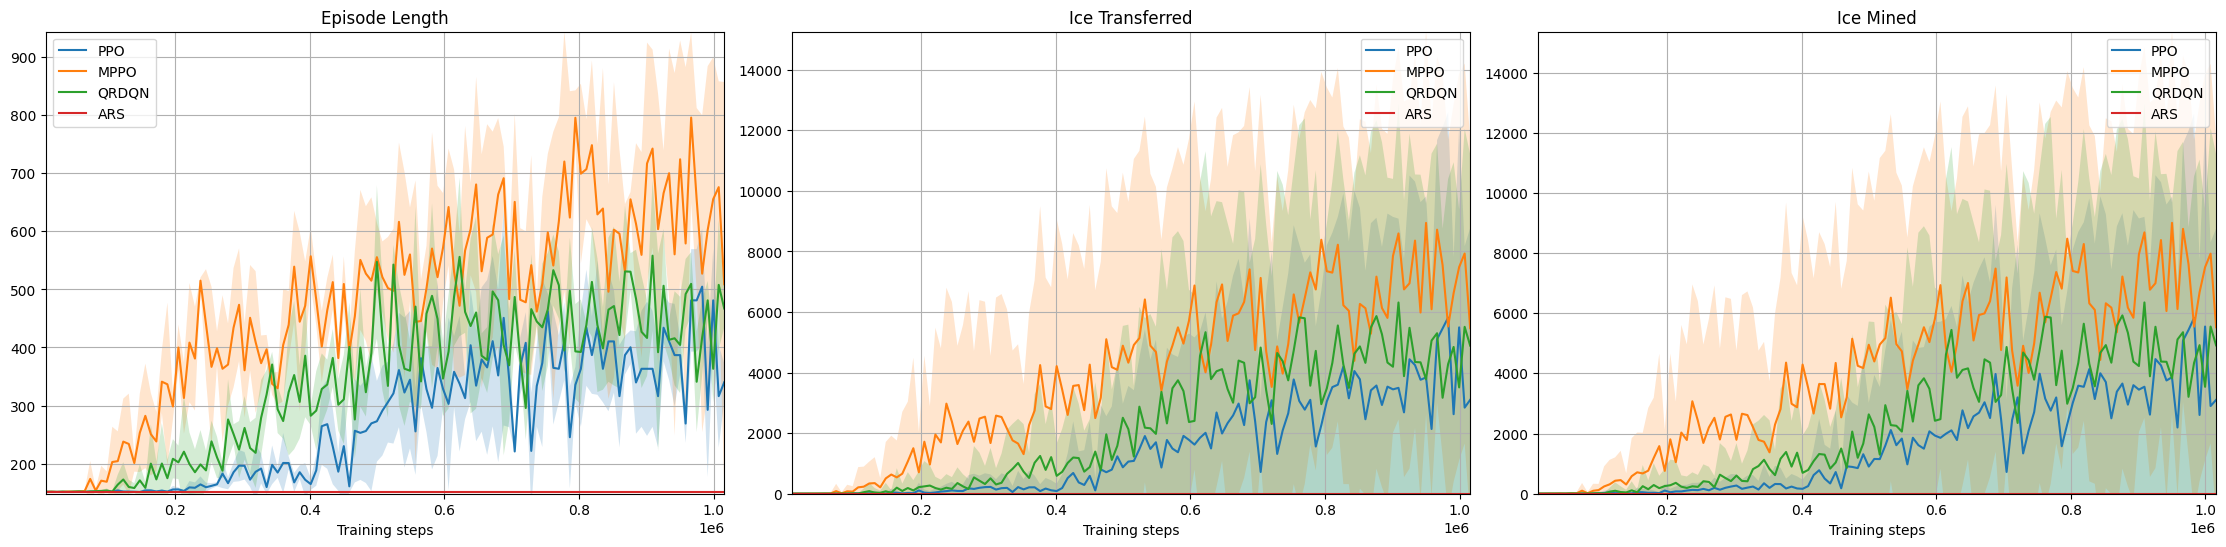
\includegraphics[width=\linewidth]{images/results_singleunit/total_single_unit.png}
        \captionsetup{justification=justified, singlelinecheck=false, width=1\linewidth, labelfont=bf} 
        \caption{In a comprehensive final comparison of the top-performing policy gradient algorithms (PPO, M-PPO), the value-based algorithm (QR-DQN), and the sole neuro-evolution algorithm (ARS).}
        \label{fig:total_single_unit}
\end{figure}

\noindent The data in \textcolor{deepblue}{\autoref{fig:total_single_unit}} validates a key assumption: \textbdd{masking out invalid actions in the environment}, thereby limiting the exploration space, proves \textbdd{advantageous in early training}. This approach accelerates learning by preventing illegal moves. The ongoing cost of recalculating masks in later training stages yields diminishing returns, as the model naturally learns to avoid meaningless actions over time. Nonetheless, this trade-off is highly favorable, as the early acceleration is essential to prevent the agent from getting stuck in local optima, and the minor decrease in training speed during later phases is acceptable. \textbdd{ARS falls short of expectations} in more complex environments characterized by large action spaces and sparse rewards. The algorithm struggles to navigate such environments effectively, particularly because rubble must be destroyed for ice to be mined. Without heavy reward shaping, it is highly improbable for a random search algorithm like ARS to consistently identify the correct rubble location and continue digging until the rubble is destroyed, leading to ice mining and reward collection.

\bigskip

\noindent Based on the observed results, we decided to \textbdd{transition from the single-unit setting to a multi-agent environment} using the \textbdd{M-PPO algorithm}. This decision was influenced by M-PPO's stable learning behavior facilitated by clipping techniques and its capability to converge to an optimal policy by masking out invalid actions within the environment.


\section{Monolithic Approach}
\label{sec:monolithic-approach-results}

\noindent In this section, we analyze various results of our monolithic approach (\autoref{sec:monolithic-approach}), focusing on its \textbdd{potential and limitations} in the Lux AI environment. We compare different network architectures, including a U-net type neural network with two distinct bottleneck techniques (\autoref{fig:Bottlenecks}) and another architecture that maintains the original size of the input observation (\autoref{sec:monolithic-network}). The \textbdd{BottleNet} architecture achieves the creation of a \textbdd{class system} within the network, allowing it to produce a segmentation map where each pixel corresponds to a specific action that a unit can take, such as digging or recharging. In contrast, the DashNet architecture maintains the original height and width dimensions, effectively mapping each piece of information provided by a pixel to an action. This mapping is achieved while also considering other parts of the network through convolution operations.

\bigskip

\noindent The addition of \textbdd{squeeze-and-excitation layers} (\autoref{subsec:se}) in our architecture played a critical role in improving our mapping and classification objectives. Initially, when these layers were omitted, we observed a notable decrease in model performance. Squeeze-and-excitation layers dynamically modulate the importance of feature maps, thereby increasing their contribution to accurate mapping from observation to input. Notably, the feature channel representing ice resources on the map exhibited significant influence on the digging action when combined with the unit map.

\bigskip

\noindent We introduced a \textbdd{novel masking method} designed to align with the principles of Proximal Policy Optimization, aiming to constrain the magnitude of updates through its clipping mechanism. This method involved invalidating all actions for map spaces devoid of entities, except for the no-operation action, thereby establishing \textbdd{determinism in empty pixels}. This deterministic approach introduced minimal noise to updates, as updates primarily occurred in regions occupied by entities. Specifically, on a $48\times48$ map typically involving $30$ entities, with approximately $4$ factories and $26$ units, out of $2,304$ pixels, updates were concentrated in areas where entities were present. Consequently, our masking policy utilized small updates, mitigating the risk of policy collapse or entrapment in local optima. During training, we consistently observed improvements in performance without encountering any instabilities. Throughout updates, \textbdd{KL divergence remained minimal} with respect to the policy, typically falling within the expected range for PPO, between 0 and 1. This suggests that the probability of a certain action doubled at most, indicating that $P$ was approximately twice as likely as $Q$ for that specific outcome, measured on a binary logarithmic scale. Moreover, we observed a minimal clipping fraction for gradient updates, typically ranging between 0.1 and 0.2, indicating that the \textbdd{model did not attempt overly aggressive updates}.

\subsection{DashNet vs BottleNet}

\begin{figure}[htbp]
    \centering
    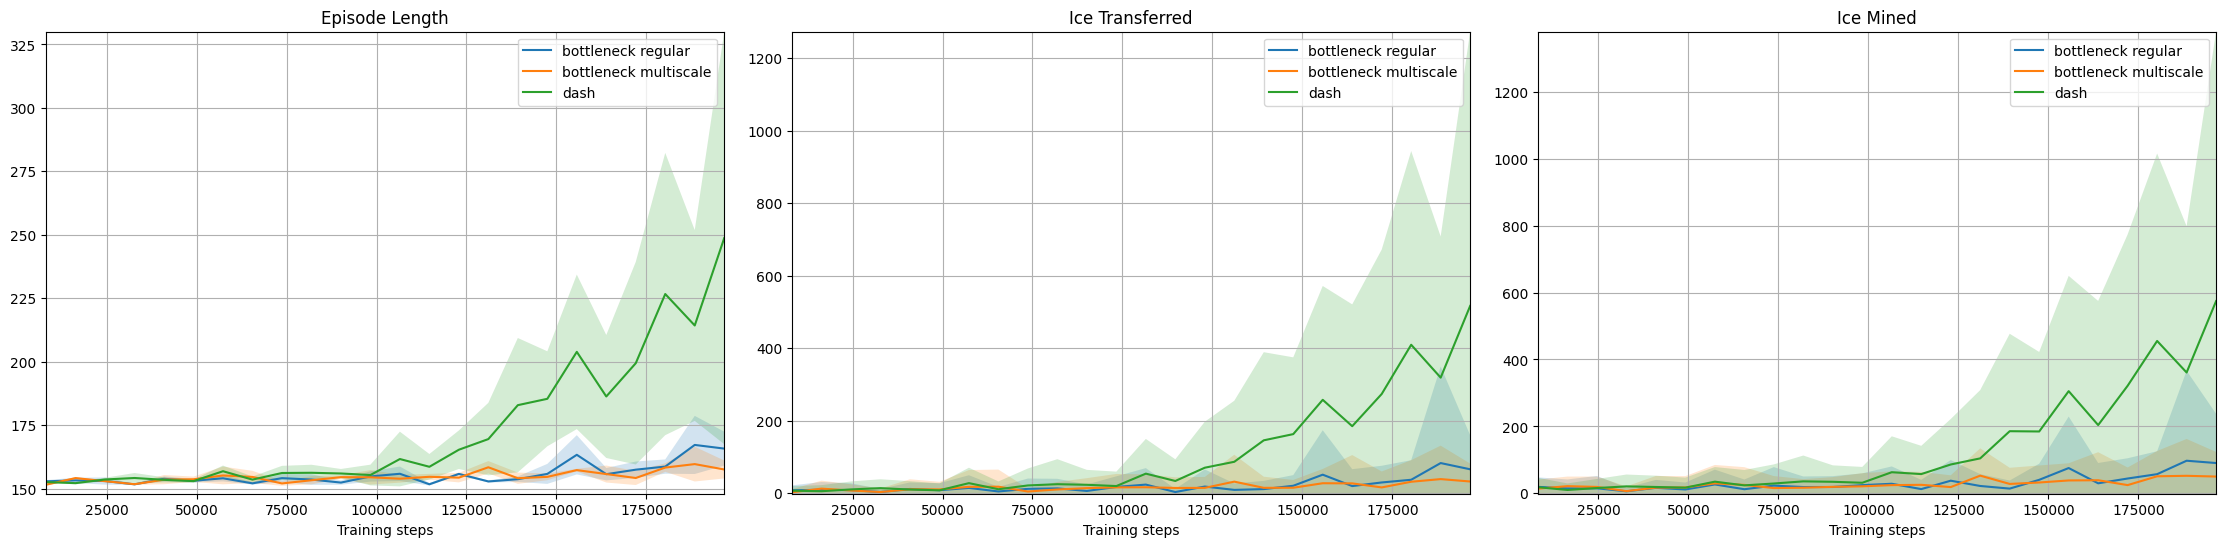
\includegraphics[width=1\linewidth]{images/results_monolithic/mono_results.png}
    \captionsetup{justification=justified, singlelinecheck=false, width=1\linewidth, labelfont=bf} 
    \caption[]{The plot compares the performance of the monolithic approach in terms of evaluation metrics, including the length of episodes, ice transferred by units, and ice mined. The data clearly demonstrates the superiority of DashNet over both BottleNets. DashNet shows improvement across all aspects, achieving higher training speeds, similar fluctuations, stable learning behavior, and consistent enhancement, particularly notable after 81,920 steps.}
    \label{fig:mono_results}
\end{figure}


\noindent \autoref{fig:mono_results} presents the performance of both algorithms based on evaluation metrics such as average \textbdd{episode length, ice dug, and ice transferred}. The episode length metric serves the same purpose as in the single-unit testbench (\autoref{sec:single-unit-testbench-results}), evaluating the ability of the global policy to sustain factories. Ice dug and ice transferred metrics are employed for \textbdd{alignment checking}, as these actions were positively rewarded in the environment. The results represent data from three trials, trained from scratch up to 204,800 steps. This extended training duration was necessary due to SB3's lack of self-play support during development, doubling our initial target of 102,400 steps. Thus, we provided the model with the same amount of data, albeit from the same on-policy perspective. Batch sizes and rollout steps were also doubled to align with our 102,400-step target. While all algorithms showed an increasing trend in performance, the \textbdd{U-net architecture fell behind after 81,920 steps}. This suggests that downsizing the observation space to a small bottleneck size and attempting to reconstruct a class map through on-policy optimization results in smaller updates, leading to slower learning compared to maintaining the original input size and finding a correct same-size mapping in neural network space.

\begin{table}[h!]
    \centering
    \begin{tabular}{|c|c|}
        \hline
        \textbf{Algorithm} & \textbf{Longest Evaluation Episode} \\
        \hline
        Simple BottleNet     & 178 steps \\
        Multiscale BottleNet & 167 steps \\
        \textbf{DashNet}    & \textbf{325 steps} \\
        \hline
    \end{tabular}
    \captionsetup{justification=justified, singlelinecheck=false, width=1\linewidth, labelfont=bf} 
    \captionof{table}{The table displays the longest evaluation episode, indicating which episode out of the total 274 (derived from 12 episodes across 25 evaluation phases) had the longest surviving factory (higher is better).}
    \label{tab:mono-results-table}
\end{table}

\subsection{DashNet Convergence Study}

\noindent As for a final study, we aimed to assess the convergence potential of the superior DashNet model by \textbdd{extending its training duration} to 1 million steps, a fivefold increase compared to previous trials. We also explored alternative configurations, such as removing normalization layers and residual blocks from the network, but found that they led to poor performance. Additionally, extensive ablation studies were conducted as part of the hybrid method, detailed in \autoref{subsec:ablation}, to examine the significance of regularization techniques, network depth, and factory placement and bidding heuristics.


\begin{figure}[htbp]
    \centering
    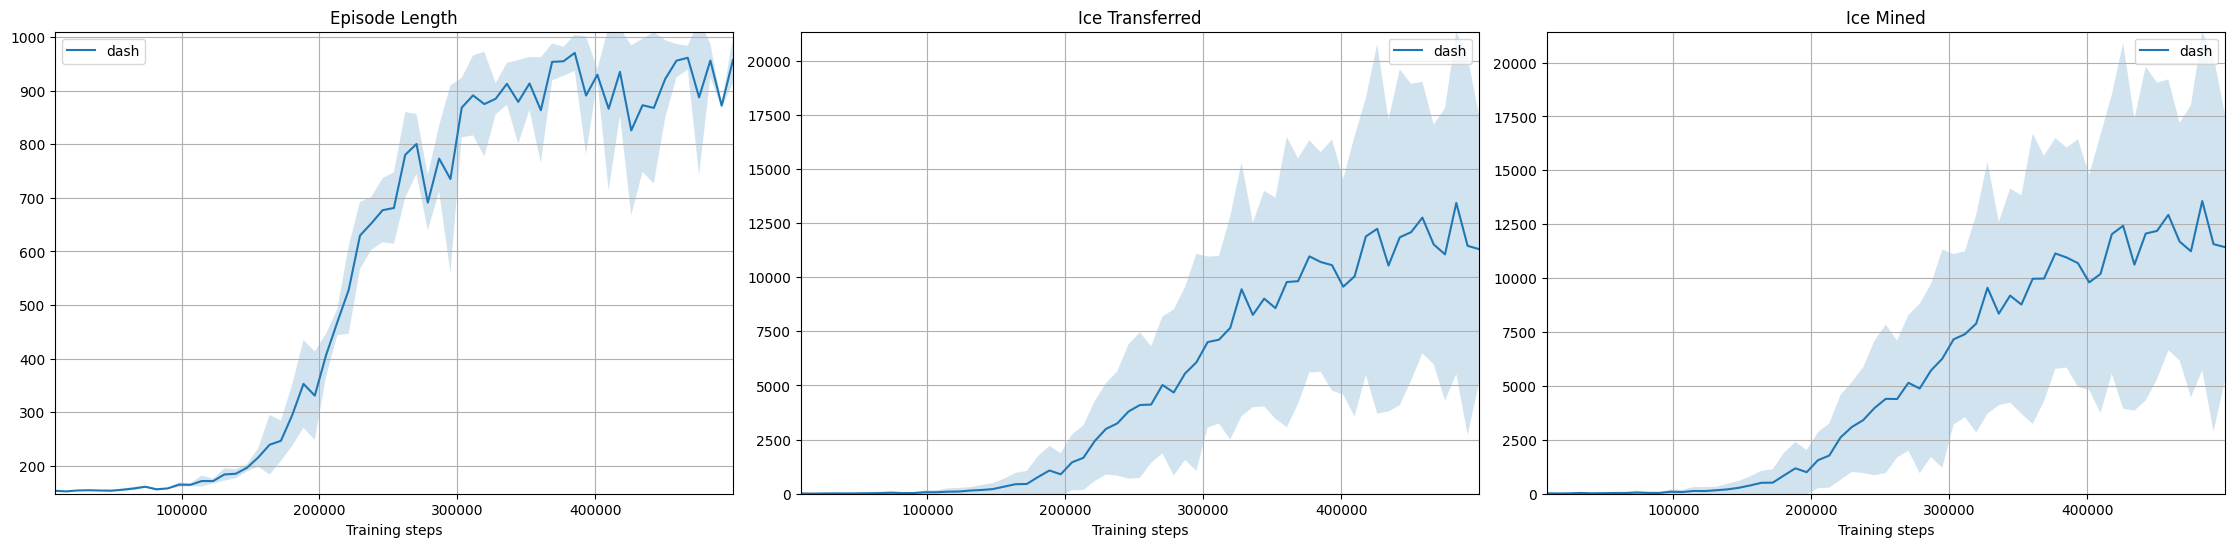
\includegraphics[width=1\linewidth]{images/results_monolithic/dash_1m.png}
    \captionsetup{justification=justified, singlelinecheck=false, width=1\linewidth, labelfont=bf} 
    \caption[]{The image illustrates the results obtained from the \textbdd{DashNet architecture}, averaged over three trial runs, with each trained until 507,904 training steps. The plots indicate that the algorithm converges around an average episode length of 1000, exhibiting minor fluctuations attributed to sparse updates resulting from architectural specifications.}
    \label{fig:mono-dash-1M}
\end{figure}

\bigskip

\noindent \autoref{fig:mono-dash-1M} illustrates the model's progression beyond the initial exploration phase, demonstrating a \textbdd{snowball effect} in algorithm performance as it refines its policy. While the model achieved an average of \textbdd{1024 steps in $\mathbf{95\%}$ of the evaluation environments} after 507,904 training steps, this progress was achieved at a significant cost and slow pace. The combination of the monolithic approach exhibited great potential; however, there are numerous optimization opportunities for further improvement, despite the semi-paradoxical nature of its learning dynamics. These optimization opportunities are addressed in the hybrid approach (\autoref{sec:hybrid-approach-results}).

\bigskip

\noindent Consistent updates led to the achievement of a \textbdd{convergent policy}; however, efficiency remains a concern. Given our monolithic approach, especially during initial training stages, \textbdd{suboptimal actions are often reinforced}. This is because only a minority of entities exhibit positive behavior, while the majority engage in non-beneficial actions. To address this, the model requires active engagement from at least half of the entities, plus one, in positive actions, while the remaining entities may persist with suboptimal actions, thereby influencing the overall learning dynamics of the model.

\bigskip

\subsection{Against the Odds}

\noindent In the following, we analyze a hypothetical scenario, in which we train a model from scratch and consider a map with 30 entities. These entities include 4 factories, 4 heavy units, and 22 light units. In this scenario, we can hypothesize the following: Factory actions do not yield immediate rewards directly to the model. However, through the production of units, positive actions are indirectly initiated in all instances. When a factory depletes its resources, its sole feasible action is \textbdd{no operation}, which inherently benefits the model as it facilitates resource conservation. Thus, \textbdd{factories consistently contribute positively to the model's performance}.

\bigskip

\noindent When considering units, our analysis must be split to address heavy units separately from light units. For heavy units, achieving a rewarding action is exceedingly unlikely. A hypothetical assessment may be outlined as follows: Typically, units have access to approximately 5 possible actions on average, due to the masking of invalid actions. However, in most cases, only one action results in a rewarding outcome. Moreover, the likelihood of achieving a reward is further diminished, as it necessitates a sequence of optimal actions. Heavy units are generally capable of achieving this within 5 steps, resulting in an individual \textbdd{heavy unit having a probability of only $\mathbf{4\%}$ to attain a possible reward}. To ascertain the probability of at least 3 units achieving this, we resort to the binomial distribution (\cite{enwiki:1223310929}). The probability mass function of a binomial distribution is given by:

\begin{equation}
P(X = k) = \binom{n}{k} p^k (1-p)^{n-k},
\label{eq:binomial}
\end{equation}

where

\begin{itemize}[itemsep=4pt, parsep=0pt]
    \item \( n \) is the number of trials (4 - heavy, 22 - light),
    \item \( k \) is the number of successful trials (3 - heavy, 13 - light),
    \item \( p \) is the probability of success on a single trial \( \left( (\frac{1}{5})^5 \text{ - heavy},  (\frac{1}{5})^{10}  \text{ - light} \right) \).
\end{itemize}



\noindent For heavy units, this yields a probability of approximately $2.45 \times 10^{-4}$. Conversely, for light units, with a much larger population, where a rewarding action occurs on average every 10 steps, \textbdd{the probability is even smaller}, falling within the range of $1 \times 10^{-61}$. To appropriately weigh these probabilities, it's important to consider that heavy units offer 10 times more opportunities for rewards in terms of magnitude in a single step. However, even after adjusting for this factor, the final probability remains \textbdd{exceedingly small and negligible}, akin to winning the lottery six times in a row or achieving a perfect shuffle of a 52-card deck. It's essential to note that these calculations are approximate and valid only prior to the first update to the model, as action probabilities follow a uniform distribution. 

\bigskip

\noindent The purpose of the above calculations was to provide an \textbdd{order of magnitude} type estimation (rather than precise numerical calculations), in order to demonstrate the unlikeliness of the model achieving a significant reward, and thus a substantial update, at the beginning of the training phase. Naturally, as the model learns better policies, these probabilities increase, leading to higher chances of learning the optimal action for a given state. Given the sparsity of the monolithic method and the myriad optimization possibilities it presents, we decided to focus our efforts on evaluating our novel proposal of trajectory separation and a hybrid approach for PPO.

\bigskip

\section{Hybrid Approach}
\label{sec:hybrid-approach-results}

\noindent In this section, our primary focus will be on showcasing the effectiveness of our technique called \textbdd{trajectory separation} (\autoref{subsec:grouping}) to demonstrate its potential for improving the hybrid architecture (\autoref{sec:hybrid-approach}). In addition, we will explore potential enhancements and limitations of the method, including examining the components of trajectory separation to determine the specific factors that contribute to the improvement of performance. We will also conduct a comparative analysis between the trajectory-separated hybrid, \textbdd{pixel-to-pixel} architecture (\autoref{par:pixel-to-pixel}) and existing solutions for the Lux AI competition. At the end of the section, an ablation study will be carried out, analyzing the methods in addition to trajectory separation.

\bigskip

\noindent In the subsequent configurations, factories, and units will be organized into distinct groups, each with aggregated outputs and trajectories. Groups can exhibit various characteristics, from global groups encompassing all entities of a specific type to individual groups in which each entity functions as its own separate group. In this study, we illustrate the significance of distinct trajectories within a multi-agent setting and investigate various approaches for distributing rewards among the agents. All of the experiments shared a common training objective, which was to train the units to keep the factories alive until the end of the game, spanning 1,000 steps. In the following experiments, we will employ the metrics specified in \autoref{sec:hybrid-metrics}. These metrics include the length of an episode, the aggregate amount of ice transferred to factories within a given episode, and the count of operational factories at each environment step, normalized by the maximum episode duration.

\bigskip

\noindent The experiments consist of three separate runs, each utilizing different seeds and running for a total of 102,400 steps (25 training cycles with a 4,096-step batch size). We felt the difference between variants could be sufficiently highlighted in this step range. Contrary to the \textbdd{single-unit} test bench (\autoref{sec:single-unit-testbench-results}) and the \textbdd{monolithic approach} test (\autoref{sec:monolithic-approach-results}), in this scenario, \textbdd{both players are active} and performing actions simultaneously. The \textbdd{same model}, as detailed in \autoref{sec:hybrid-network-architecture}, was used for both players and was trained on their collective trajectories. Following each training cycle, we ran an evaluation of the model by executing 12 distinct environments until the conclusion of the matches. These environments were seeded differently for each of the three runs. The evaluation process yielded 36 data points per training cycle for environment-specific metrics, specifically the metric of \textttdb{Episode Length}. Additionally, by considering each player separately, there were 72 data points for player-specific metrics, including \textttdb{Ice Transferred} and \textttdb{Average Factory Alive}. The lines on the charts visually represent the metrics' means, while the shaded area shows the standard deviation. In addition to the charts, tables are included to make comparisons easier. The columns \textttdb{Final Ice Transferred} and \textttdb{Final Episode Length} refer to the metrics collected at the last evaluation of the model. The mean value is presented, along with the standard deviation in brackets. The \textttdb{X\% of Episodes Finished by} metrics measure how long it took for the agents to learn how to keep the factories alive until the end of the game in terms of environment steps. The percentage indicates the ratio of evaluation environments that resulted in a finished episode, which is an episode where at least one factory survived from both players until 1,000 steps.

\subsection{Trajectory Separation} \label{sec:trajectory-separation}

\subsubsection{Global Trajectory vs Separated Trajectories}

\noindent An initial experiment was done to see what effect \textbdd{separated trajectories} (\autoref{subsec:grouping}) had on how fast the agents learned. As the control group, we implemented a variant that closely resembles the original pixel-to-pixel method (\cite{chen2023emergent}) by utilizing a single \textbdd{global group} (\textttdb{"single global trajectory"}), resulting in a centralized architecture. To evaluate our more decentralized approach, we experimented with various group configurations. These configurations included the formation of distinct \textbdd{global groups} for each entity type (\textttdb{"global factories, global units"}), the creation of a single global group for one entity type while maintaining individual groups for the other (\textttdb{"global factories, separate units"}, \textttdb{"separate factories, global units"}), and the establishment of \textbdd{individual groups} for each entity (\textttdb{"separate trajectories for all entities"}). As demonstrated in \autoref{fig:hybrid_results/trajectory_separation/combined} and \autoref{tab:hybrid_results/trajectory_separation/combined}, the variants with separated trajectories perform much better compared to the global trajectory variants. The most notable improvement is the \textbdd{rate of convergence}, which resulted in the model learning to keep the factories alive until the end of the game by around the 50,000th step, which the fully global variant could not achieve at all. Upon arriving at this significant milestone, the agents continued to improve their strategies further, leading to an average transfer of more than 40,000 ice to factories throughout the 1,000 steps in an episode. The value is 13 times greater than the achievement of the global trajectory variant. The accomplishment was reached by acquiring the skill to transfer ice to all of the factories rather than solely to one, which would have been sufficient to reach the maximum episode length. We can see this by the \textbdd{average factory alive} metric, which continues to rise even after the \textbdd{episode length} levels off at the maximum possible value. The new technique also reduced the \textbdd{frequent fluctuations} of the model's performance, which hinted at unlearning the progress made by the previous steps. We suspect this was the cause of destructive behavior reinforcement, which our method avoids since agents are only rewarded for their actual work (explained in \autoref{subsec:methodcomp}). The findings of the experiment indicate that utilizing separate trajectories can offer a notable benefit to the agents' training process.

\begin{figure}[htbp]
    \centering
    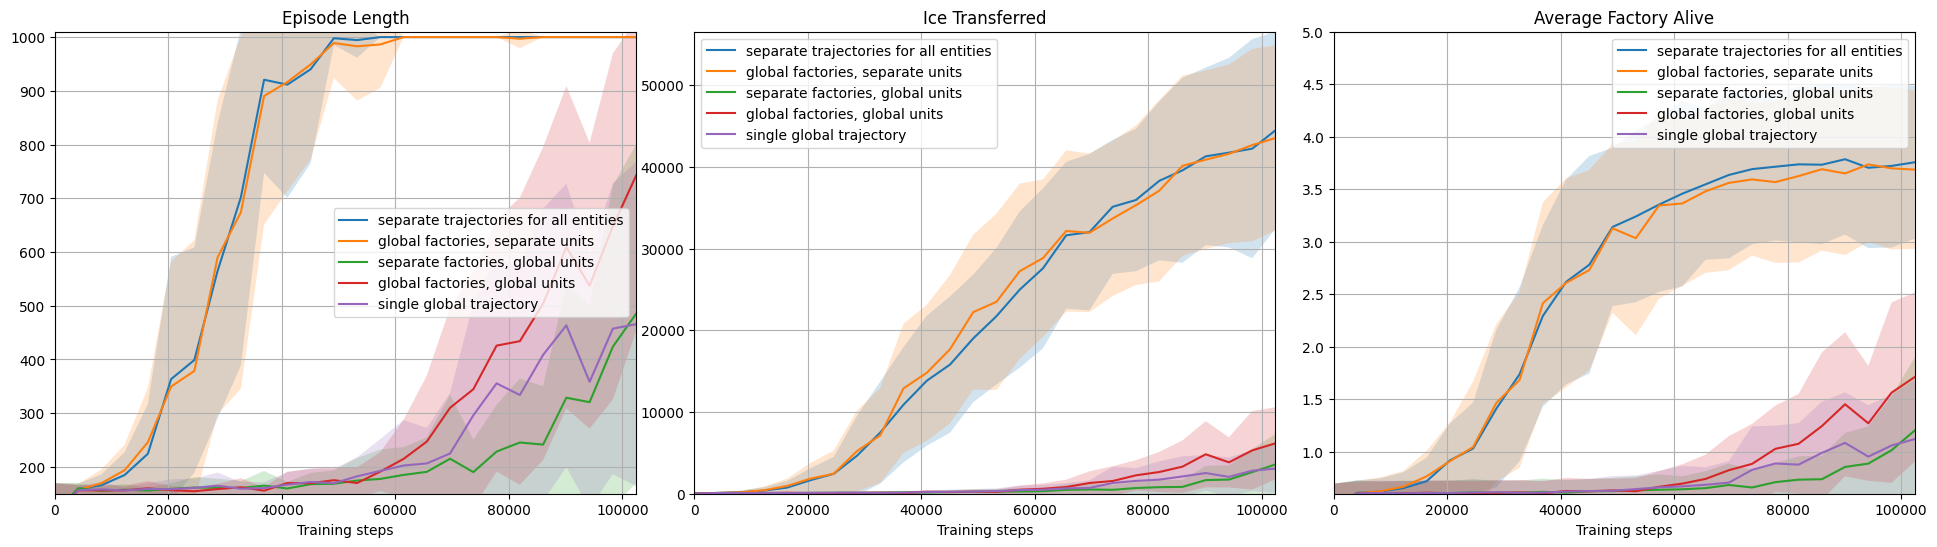
\includegraphics[width=0.95\linewidth]{images/results_hybrid/trajectory_separation/combined.png}
    \captionsetup{justification=justified, singlelinecheck=false, width=1\linewidth, labelfont=bf} 
    \caption[]{Plot comparing the usage of trajectory separation and global trajectories in terms of the length of the episodes, ice transferred by units, and number of active factories. The data presented in the figure indicates a clear improvement in all metrics thanks to the utilization of trajectory separation. In addition to faster convergence, the variants with separated trajectories exhibit reduced fluctuations in performance, thereby leading to more efficient training.}
    \label{fig:hybrid_results/trajectory_separation/combined}
\end{figure}

\begin{table}[ht]
    \footnotesize
    \renewcommand{\arraystretch}{1.2}%
    \begin{tabularx}{\textwidth}{|X|C{2.3cm}|C{2.3cm}|C{2.0cm}|C{2.0cm}|}
        \hline
\multicolumn{1}{|Y|}{\textbf{Group Name}} & \textbf{Final Ice Transferred} & \textbf{Final Episode Length} & \textbf{10\% of Episodes Finished by} & \textbf{95\% of Episodes Finished by} \\
        \hline
separate trajectories for all entities & \textbf{44,472 (12,065)} & \textbf{1,000 (0)} & \textbf{28,672 steps} & \textbf{49,152 steps} \\
global factories, separate units & 43,528 (11,327) & \textbf{1,000 (0)} & \textbf{28,672 steps} & \textbf{49,152 steps} \\
separate factories, global units & 3,573 (3,753) & 485 (315) & 98,304 steps & - \\
global factories, global units & 6,162 (4,413) & 742 (290) & 81,920 steps & - \\
single global trajectory & 3,066 (2,996) & 466 (302) & 102,400 steps & - \\
        \hline
    \end{tabularx}
    \medskip
    \captionsetup{justification=justified, singlelinecheck=false, width=1\linewidth, labelfont=bf} 
    \caption{Table comparing the usage of trajectory separation and global trajectories. The metrics featured include the amount of ice transferred by units and the length of the episodes in the evaluation phase following the last training cycle. The table also contains the observed environment steps needed until the model reaches the maximum episode length in the specified percentage of evaluation environments. The variant with completely separate trajectories was able to provide the factories with 13 times more ice after the training and has managed to reach the maximum episode length in 10\% of the evaluation environments more than 3 times faster.}
    \label{tab:hybrid_results/trajectory_separation/combined}
\end{table}

\subsubsection{Number of Optimal Trajectories}

\label{subsec:modulus-grouping}
\noindent In order to demonstrate the significance of separating the entity trajectories, we conducted an additional experiment in which we categorized the units into $N$ groups based on the modulus of their unique IDs. This categorization led to approximately \textbdd{random allocation across the groups}, enabling us to examine the optimal number of trajectories to divide our training steps into. The units were the only entities involved in the grouping, as the factories remained entirely separate during this test. The results are displayed in \autoref{fig:hybrid_results/group_size/combined} and \autoref{tab:hybrid_results/group_size/combined}. It is evident that increasing the number of trajectories resulted in a faster and more efficient training process for the agents, suggesting that the \textbdd{optimal training method} is utilizing a \textbdd{separate trajectory for all entities}.

\begin{figure}[htbp]
    \centering
    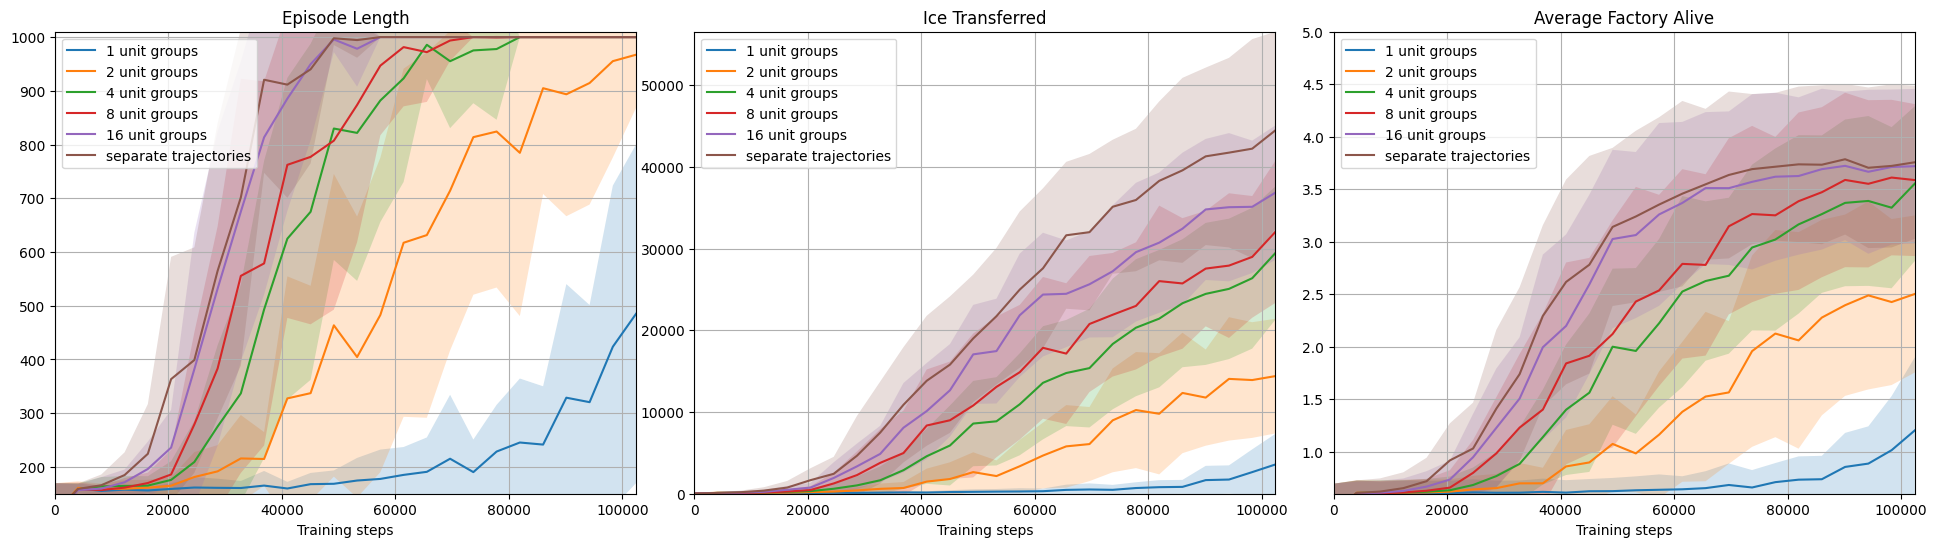
\includegraphics[width=0.95\linewidth]{images/results_hybrid/group_size/combined.png}
    \captionsetup{justification=justified, singlelinecheck=false, width=1\linewidth, labelfont=bf} 
    \caption[]{Plot comparing the performance of separating the global trajectory into $N$ separate trajectories in terms of the length of the episodes, ice transferred by units, and number of active factories. In addition to the test variants, the global and completely separate trajectory variants are also present. The figure indicates a positive correlation between the number of separate trajectories and the performance achieved on all metrics.}
    \label{fig:hybrid_results/group_size/combined}
\end{figure}

\begin{table}[ht]
    \footnotesize
    \renewcommand{\arraystretch}{1.2}%
    \begin{tabularx}{\textwidth}{|X|C{2.3cm}|C{2.3cm}|C{2.0cm}|C{2.0cm}|}
        \hline
\multicolumn{1}{|Y|}{\textbf{Group Name}} & \textbf{Final Ice Transferred} & \textbf{Final Episode Length} & \textbf{10\% of Episodes Finished by} & \textbf{95\% of Episodes Finished by} \\
        \hline
1 unit groups & 3,573 (3,753) & 485 (315) & 98,304 steps & - \\
2 unit groups & 14,388 (7,019) & 967 (99) & 57,344 steps & - \\
4 unit groups & 29,459 (8,150) & \textbf{1,000 (0)} & 36,864 steps & 77,824 steps \\
8 unit groups & 32,049 (8,701) & \textbf{1,000 (0)} & 32,768 steps & 61,440 steps \\
16 unit groups & 36,847 (8,224) & \textbf{1,000 (0)} & \textbf{28,672 steps} & 57,344 steps \\
separate trajectories & \textbf{44,472 (12,065)} & \textbf{1,000 (0)} & \textbf{28,672 steps} & \textbf{49,152 steps} \\
        \hline
    \end{tabularx}
    \medskip
    \captionsetup{justification=justified, singlelinecheck=false, width=1\linewidth, labelfont=bf} 
    \caption{Table comparing the performance of separating the global trajectory into $N$ separate trajectories. The metrics featured include the amount of ice transferred by units and the length of the episodes in the evaluation phase following the last training cycle. The table also contains the observed environment steps needed until the model reaches the maximum episode length in the specified percentage of evaluation environments. In addition to the test variants, the global and completely separate trajectory variants are also present. The table shows a massive jump in the final average episode length even by separating the global trajectory into two random groups. While the episode length metric reaches its maximum value with 4 unit groups, an increased convergence rate can be observed by using even more separate trajectories.}
    \label{tab:hybrid_results/group_size/combined}
\end{table}


\subsection{Trajectory Number Reduction}
\label{subsec:trajec_reduc}

\noindent The technique of \textbdd{trajectory separation} (\autoref{sec:trajectory-separation}) provides an optimized approach that enables efficient training of a centralized model for a multi-agent problem. However, it should be noted that the large number of trajectories does have certain limitations. Because the separated \textbdd{training examples} are tied to their respective environment steps, which are used to partition our \textbdd{mini-batches} during training, and considering that the number of trajectories can vary at each step, it is possible for the mini-batches to have an \textbdd{imbalanced number of training examples}. Given that the sizes of the matrices remain constant and padding values are used for inactive groups, this does not pose any issues regarding vectorization or memory utilization. Nevertheless, this phenomenon could potentially lead to an \textbdd{asymmetry} in the impact that each training example has on the policy loss, as the final loss is obtained by averaging all training examples. Steps with a large number of currently active groups will carry \textbdd{more significance}, whereas the impact of a group's example within a step with a low number of active groups will be \textbdd{more pronounced} compared to a group's example within a step with a higher population. This is because, on average, the former will be included in a mini-batch with fewer examples. Even if the mini-batch sizes were balanced, it would remain uncertain whether the \textbdd{increased number of trajectories} is \textbdd{advantageous} for the training process. The generation of a large number of training instances from the available environment steps introduces a \textbdd{regularization effect} to the model's training process, thereby reducing the influence of each individual instance. If the primary challenge associated with a single global trajectory is the complex action space and the \textbdd{incomprehensible singular reward value}, it is possible that by eliminating these factors, a reduced quantity of training examples may be sufficient to obtain convergence. Reducing the size of the batches while maintaining the same performance would further optimize our technique. In order to assess the impact of the aforementioned issues, we will employ two methodologies: \textbdd{agent grouping} (\autoref{sec:res-grouping}), wherein we will evaluate the performance attainable through various grouping criteria, and \textbdd{trajectory sample reduction} (\autoref{subsec:tsr}), wherein we will selectively utilize data from the top or bottom $N$ groups based on a specified metric for each step in the environment.

\subsubsection{Grouping}
\label{sec:res-grouping}

\noindent The results of the modulus test in \autoref{subsec:modulus-grouping} show a strong link between performance and the \textbdd{number of allowed separate trajectories}. The variant that was \textbdd{unconstrained} by any kind of grouping outperformed all the other variants. However, it raises the question of whether comparable performance can be attained with a \textbdd{bounded variant} by implementing a grouping rule that is beneficial for the training process. As shown in \autoref{fig:hybrid_results/group_rule/combined} and \autoref{tab:hybrid_results/group_rule/combined}, our experiment involved evaluating the effectiveness of three different grouping strategies: grouping by \textbdd{map segments} (\textttdb{"map quadrants"}), grouping by \textbdd{closest factories} (\textttdb{"closest factory"}), and grouping by \textbdd{closest heavy units} (\textttdb{"closest heavy"}). All of these groupings led to a \textbdd{bounded number of trajectories}, as the size of the map remains constant, and the number of factories can only vary between three and five. At first glance, the number of heavy units may appear to be limitless; however, the resources available to a factory only permit the production of a single heavy unit per factory. None of the groups that were tested were able to achieve performance comparable to that of the completely separated variant. Additionally, the \textbdd{number of groups remained a significant indicator of performance}. We used the \textbdd{randomly grouped} variants from \autoref{fig:hybrid_results/group_size/combined} (\textttdb{"4 unit groups"}, \textttdb{"8 unit groups"}) to see if non-random grouping rules can perform better than a random group assignment with the same number of separated trajectories. Unfortunately, all of the variants that were subjected to testing demonstrated lower performance or demonstrated comparable results to those assigned randomly. The sole exception was the \textttdb{"closest heavy"} variant; however, it still failed to outperform random assignment in terms of converging to the maximum episode length. The findings indicate that the approach of \textbdd{grouping} the trajectories of entities together in order to reduce the number of training examples \textbdd{yields poor performance}.

\begin{figure}[htbp]
    \centering
    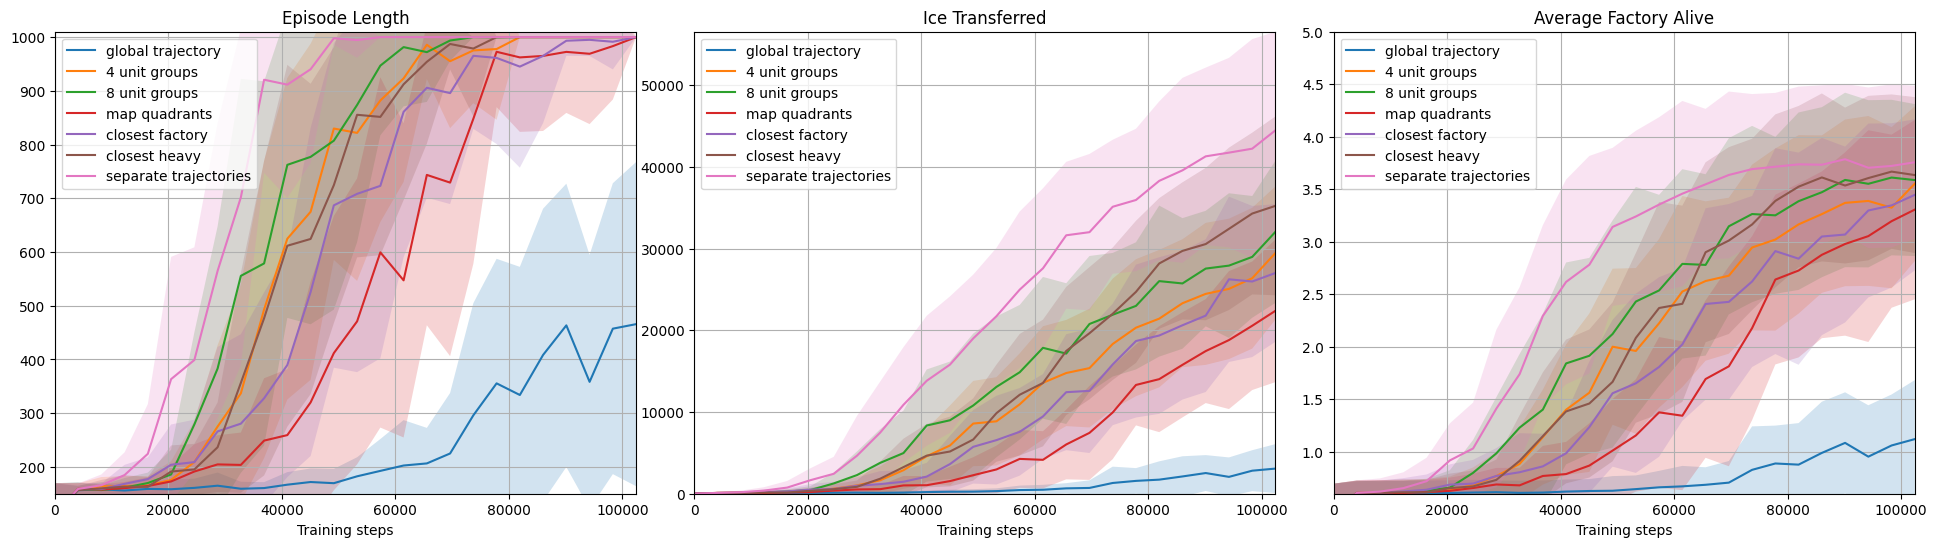
\includegraphics[width=0.95\linewidth]{images/results_hybrid/group_rule/combined.png}
    \captionsetup{justification=justified, singlelinecheck=false, width=1\linewidth, labelfont=bf} 
    \caption[]{Plot comparing the usage of different grouping rules in terms of the length of the episodes, ice transferred by units, and number of active factories. In addition to the test variants, the global and completely separate trajectory variants are also present. None of the tried variants managed to beat the separate trajectory variant in performance.}
    \label{fig:hybrid_results/group_rule/combined}
\end{figure}

\begin{table}[ht]
    \footnotesize
    \renewcommand{\arraystretch}{1.2}%
    \begin{tabularx}{\textwidth}{|X|C{2.3cm}|C{2.3cm}|C{2.0cm}|C{2.0cm}|}
        \hline
\multicolumn{1}{|Y|}{\textbf{Group Name}} & \textbf{Final Ice Transferred} & \textbf{Final Episode Length} & \textbf{10\% of Episodes Finished by} & \textbf{95\% of Episodes Finished by} \\
        \hline
global trajectory & 3,066 (2,996) & 466 (302) & 102,400 steps & - \\
4 unit groups & 29,459 (8,150) & \textbf{1,000 (0)} & 36,864 steps & 77,824 steps \\
8 unit groups & 32,049 (8,701) & \textbf{1,000 (0)} & 32,768 steps & 61,440 steps \\
map quadrants & 22,385 (8,733) & \textbf{1,000 (0)} & 53,248 steps & 98,304 steps \\
closest factory & 27,009 (8,420) & \textbf{1,000 (0)} & 45,056 steps & 94,208 steps \\
closest heavy & 35,224 (10,946) & \textbf{1,000 (0)} & 36,864 steps & 73,728 steps \\
separate trajectories & \textbf{44,472 (12,065)} & \textbf{1,000 (0)} & \textbf{28,672 steps} & \textbf{49,152 steps} \\
        \hline
    \end{tabularx}
    \medskip
    \captionsetup{justification=justified, singlelinecheck=false, width=1\linewidth, labelfont=bf} 
    \caption{Table comparing the usage of different grouping rules. The metrics featured include the amount of ice transferred by units and the length of the episodes in the evaluation phase following the last training cycle. The table also contains the observed environment steps needed until the model reaches the maximum episode length in the specified percentage of evaluation environments. In addition to the test variants, the global and completely separate trajectory variants are also present. While each grouping configuration performed better than the global trajectory variant, none could compete with the convergence rate of the completely separate trajectory variant. Grouping units by specific rules did not perform better than random grouping.}
    \label{tab:hybrid_results/group_rule/combined}
\end{table}

\subsubsection{Train Sample Reduction}
\label{subsec:tsr}

\noindent Given that all grouping methods performed less effectively than completely separate trajectories for all entities, we attempted an alternative approach to ensure a more consistent number of training examples at each step. Our technique, referred to as \textbdd{train sample reduction}, involves selecting the top $N$ examples from each step and training the model exclusively on those chosen examples. This action accomplishes two objectives. Firstly, it establishes an \textbdd{upper limit for the train examples}, thereby ensuring that the influence of each group's action remains relatively consistent, regardless of the number of other active groups. Secondly, in theory, by selecting only the most relevant examples at each step, we should be capable of \textbdd{accelerating the training process} of the model in terms of the number of environment steps and the amount of time required. In the following experiments, we utilize completely separated trajectories for all variants and perform the sample reduction solely on the train examples of units.

\bigskip

\noindent In order to first determine the optimal metric for selecting the desired subset of examples by, we conducted an experiment. We tried selecting the top $N=1$ samples by using various sampling techniques, including \textbdd{random sampling} (\textttdb{"random 1"}), \textbdd{top advantage value} (\textttdb{"top 1 advantage"}), \textbdd{top absolute advantage value} (\textttdb{"top 1 absolute advantage"}) and \textbdd{top return value} (\textttdb{"top 1 return"}). Among all of these variations, the subset that includes the examples with the \textbdd{greatest advantage value} achieved the highest performance, as evidenced by the results presented in \autoref{fig:hybrid_results/trajectory_sample_reduction/combined} and \autoref{tab:hybrid_results/trajectory_sample_reduction/combined}. Interestingly, utilizing solely the example with the \textbdd{most prominent advantage value} exhibited \textbdd{almost the same performance} as employing all of the train examples. Consequently, we decided to investigate sampling by this metric further, with different $N$ values.

\begin{figure}[htbp]
    \centering
    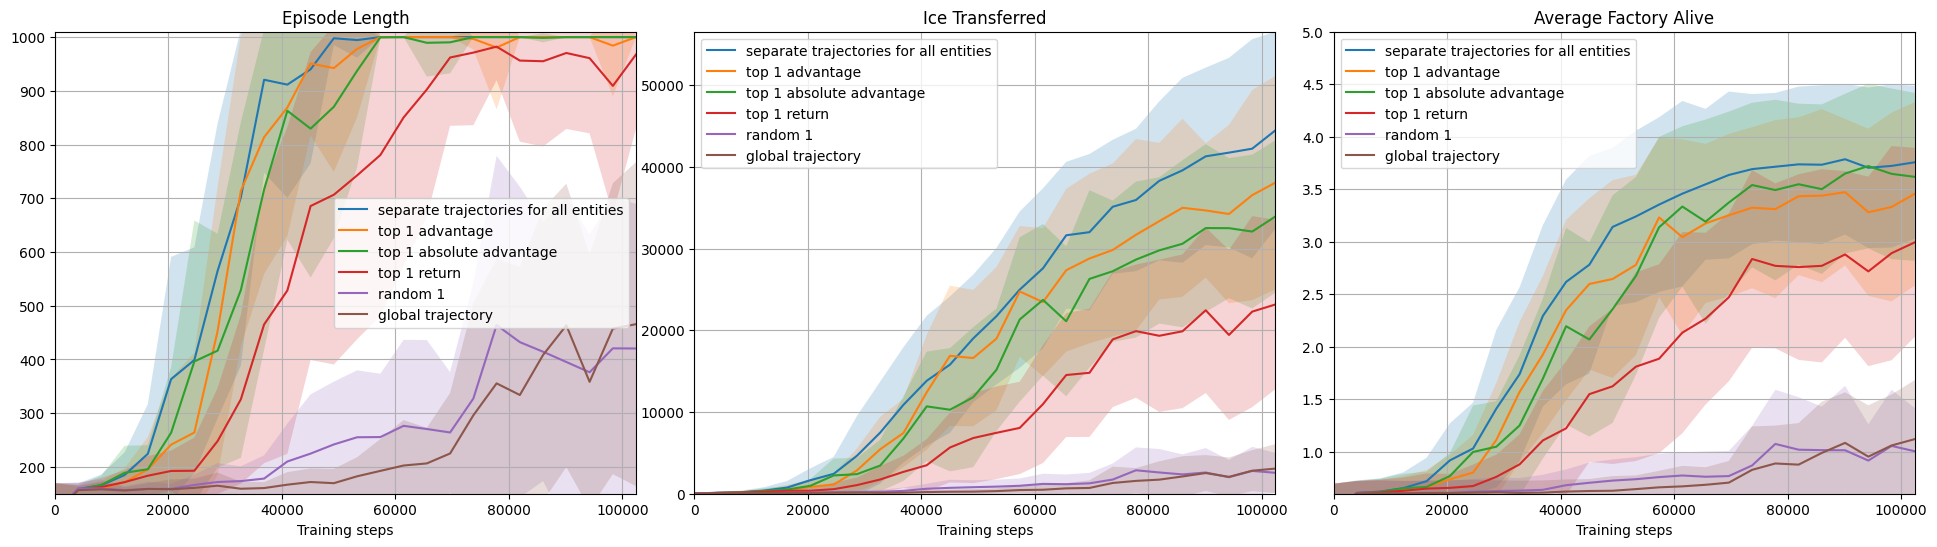
\includegraphics[width=0.95\linewidth]{images/results_hybrid/trajectory_sample_reduction/combined.png}
    \captionsetup{justification=justified, singlelinecheck=false, width=1\linewidth, labelfont=bf} 
    \caption[]{Plot comparing the different methods of trajectory sample reduction in terms of the length of the episodes, ice transferred by units, and number of active factories. In addition to the test variants, the global and completely separate trajectory variants are also present. Randomly selecting a single example at each step has the same effect as using a global trajectory. Out of all the sampling methods tried, selecting by advantage is the most prominent, leading to almost the same performance as using all data.}
    \label{fig:hybrid_results/trajectory_sample_reduction/combined}
\end{figure}

\begin{table}[ht]
    \footnotesize
    \renewcommand{\arraystretch}{1.2}%
    \begin{tabularx}{\textwidth}{|X|C{2.3cm}|C{2.3cm}|C{2.0cm}|C{2.0cm}|}
        \hline
\multicolumn{1}{|Y|}{\textbf{Group Name}} & \textbf{Final Ice Transferred} & \textbf{Final Episode Length} & \textbf{10\% of Episodes Finished by} & \textbf{95\% of Episodes Finished by} \\
        \hline
separate trajectories for all entities & \textbf{44,472 (12,065)} & \textbf{1,000 (0)} & \textbf{28,672 steps} & \textbf{49,152 steps} \\
top 1 advantage & 38,072 (13,071) & \textbf{1,000 (0)} & 32,768 steps & 57,344 steps \\
top 1 absolute advantage & 33,926 (9,324) & \textbf{1,000 (0)} & 32,768 steps & 57,344 steps \\
top 1 return & 23,156 (10,369) & 968 (138) & 40,960 steps & - \\
random 1 & 2,550 (2,434) & 420 (269) & 77,824 steps & - \\
global trajectory & 3,066 (2,996) & 466 (302) & 102,400 steps & - \\
        \hline
    \end{tabularx}
    \medskip
    \captionsetup{justification=justified, singlelinecheck=false, width=1\linewidth, labelfont=bf} 
    \caption{Table comparing the different methods of trajectory sample reduction. The metrics featured include the amount of ice transferred by units and the length of the episodes in the evaluation phase following the last training cycle. The table also contains the observed environment steps needed until the model reaches the maximum episode length in the specified percentage of evaluation environments. In addition to the test variants, the global and completely separate trajectory variants are also present. The table shows how selecting a single train example from each step by the right metric could approximate the training performance on all data. The advantage value proved to be the best metric for sampling.}
    \label{tab:hybrid_results/trajectory_sample_reduction/combined}
\end{table}

\bigskip

\noindent We tested the impact of selecting different numbers of examples with the highest advantage values from each environment step. Specifically, we tested the effects of taking 1, 2, 4, 8, and 16 such examples. The results are presented in \autoref{fig:hybrid_results/trajectory_sample_reduction_advantage/combined} and \autoref{tab:hybrid_results/trajectory_sample_reduction_advantage/combined}. Curiously, the inclusion of additional examples does not appear to significantly enhance performance. In fact, the rate of convergence is \textbdd{slightly hindered} when the sample size is increased from 4 to 16. This implies that the \textbdd{significance of an entity's action} may be \textbdd{diminished} by the multitude of other actions currently occurring in the surrounding environment, making the action less dominant in the loss calculation. By reducing the number of separate training examples and subsequently removing unnecessary data beforehand, we can help the convergence of the model. The slight edge exhibited by the sampled variants could also potentially be attributed to avoiding the problem of changing batch sizes, although a definitive conclusion cannot be drawn. We also cannot exclude the possibility that the observed, relatively small differences are due to \textbdd{sampling noise}.

\begin{figure}[ht]
    \centering
    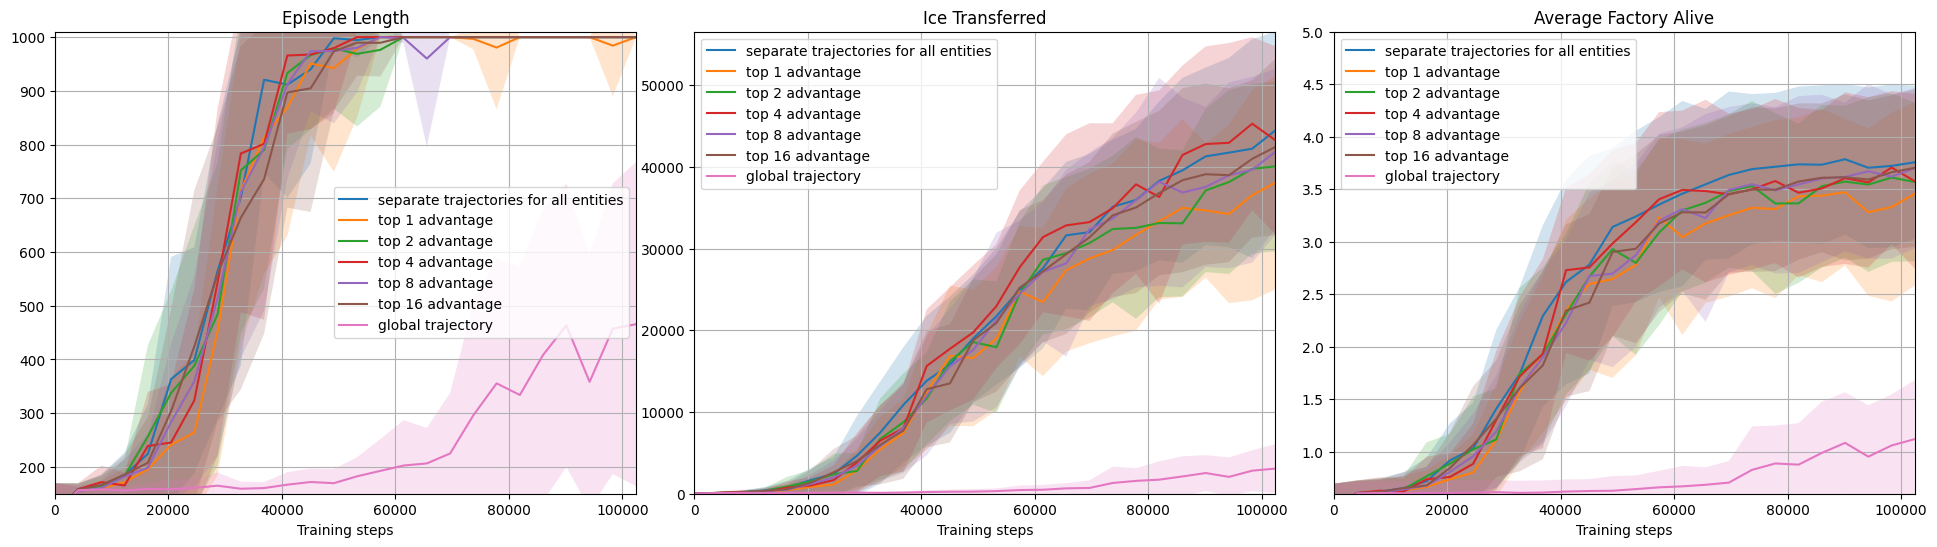
\includegraphics[width=0.95\linewidth]{images/results_hybrid/trajectory_sample_reduction_advantage/combined.png}
    \captionsetup{justification=justified, singlelinecheck=false, width=1\linewidth, labelfont=bf} 
    \caption[]{Plot comparing the performance of sampling train examples based on the advantage values in terms of the length of the episodes, ice transferred by units, and number of active factories. In addition to the test variants, the global and completely separate trajectory variants are also present. Increasing the number of sampled values appears to have minimal effect on performance, leading us to believe that the main benefit of utilizing a larger training set is to find outstandingly beneficial examples.}
    \label{fig:hybrid_results/trajectory_sample_reduction_advantage/combined}
\end{figure}

\begin{table}[ht]
    \footnotesize
    \renewcommand{\arraystretch}{1.2}%
    \begin{tabularx}{\textwidth}{|X|C{2.3cm}|C{2.3cm}|C{2.0cm}|C{2.0cm}|}
        \hline
\multicolumn{1}{|Y|}{\textbf{Group Name}} & \textbf{Final Ice Transferred} & \textbf{Final Episode Length} & \textbf{10\% of Episodes Finished by} & \textbf{95\% of Episodes Finished by} \\
        \hline
separate trajectories for all entities & \textbf{44,472 (12,065)} & \textbf{1,000 (0)} & 28,672 steps & \textbf{49,152 steps} \\
top 1 advantage & 38,072 (13,071) & \textbf{1,000 (0)} & 32,768 steps & 57,344 steps \\
top 2 advantage & 40,053 (10,402) & \textbf{1,000 (0)} & \textbf{24,576 steps} & 61,440 steps \\
top 4 advantage & 43,246 (11,518) & \textbf{1,000 (0)} & 28,672 steps & \textbf{49,152 steps} \\
top 8 advantage & 41,855 (10,159) & \textbf{1,000 (0)} & 28,672 steps & 57,344 steps \\
top 16 advantage & 42,433 (10,792) & \textbf{1,000 (0)} & \textbf{24,576 steps} & 53,248 steps \\
global trajectory & 3,066 (2,996) & 466 (302) & 102,400 steps & - \\
        \hline
    \end{tabularx}
    \medskip
    \captionsetup{justification=justified, singlelinecheck=false, width=1\linewidth, labelfont=bf} 
    \caption{Table comparing the performance of sampling train examples based on the advantage values. The metrics featured include the amount of ice transferred by units and the length of the episodes in the evaluation phase following the last training cycle. The table also contains the observed environment steps needed until the model reaches the maximum episode length in the specified percentage of evaluation environments. In addition to the test variants, the global and completely separate trajectory variants are also present. Increasing the number of advantage-sampled values did not appear to have a significant effect on performance.}
    \label{tab:hybrid_results/trajectory_sample_reduction_advantage/combined}
\end{table}

\bigskip

\noindent We were also interested in investigating the performance that can be achieved through \textbdd{random sampling}. We conducted an experiment examining the performance of different numbers of random samples, specifically 1, 2, 4, 8, and 16. The aforementioned variants were subsequently compared to the established, completely separate, and global variants. The results are available in \autoref{fig:hybrid_results/trajectory_sample_reduction_random/combined} and \autoref{tab:hybrid_results/trajectory_sample_reduction_random/combined}. Using a random sampling approach cannot provide comparable performance to utilizing the entire dataset. As expected, the performance improved as we increased the number of sampled examples, consistent with the random grouping observed in the trajectory separation experiment (\autoref{subsec:modulus-grouping}).

\begin{figure}[htbp]
    \centering
    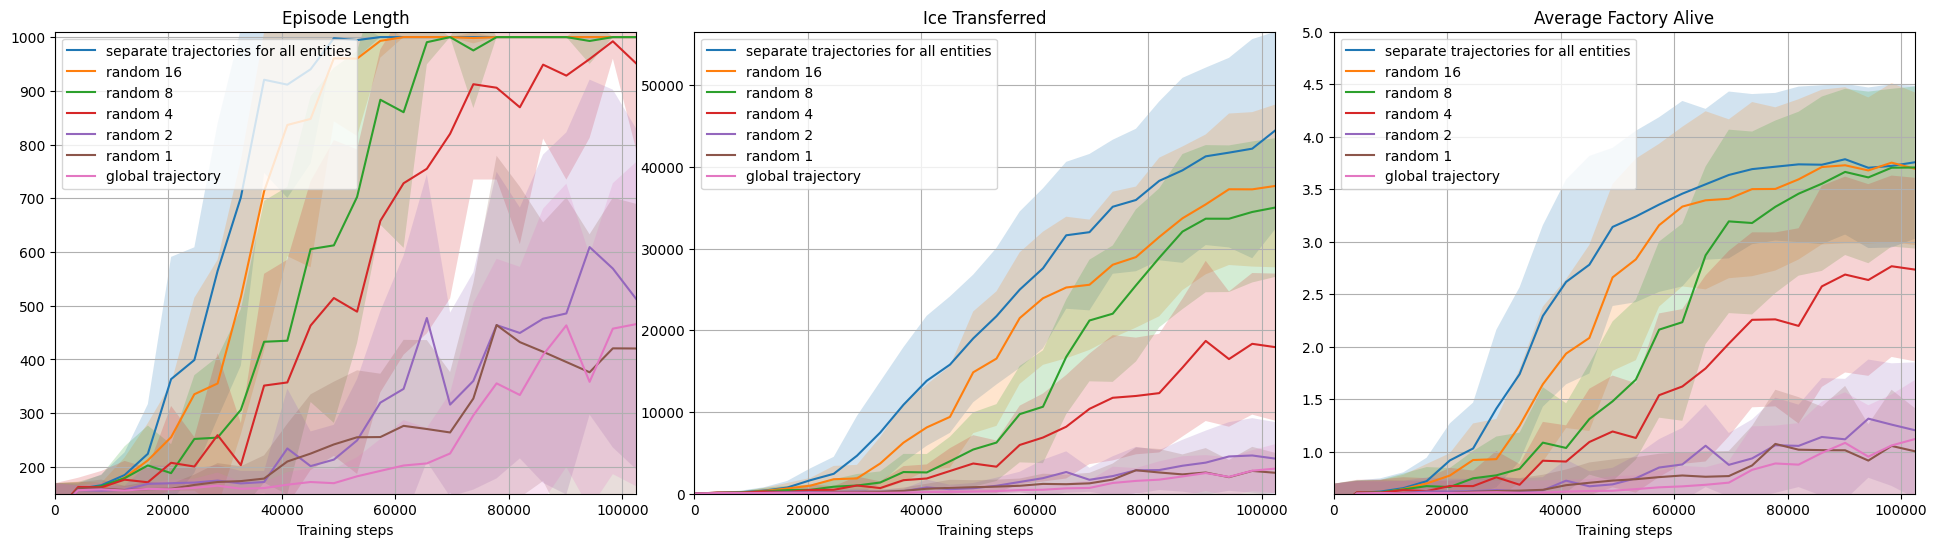
\includegraphics[width= 0.95\linewidth]{images/results_hybrid/trajectory_sample_reduction_random/combined.png}
    \captionsetup{justification=justified, singlelinecheck=false, width=1\linewidth, labelfont=bf} 
    \caption[]{Plot showcasing the performance of random train example sampling in terms of the length of the episodes, ice transferred by units, and number of active factories. In addition to the test variants, the global and completely separate trajectory variants are also present. As expected, more randomly sampled trajectories caused better performance.}
    \label{fig:hybrid_results/trajectory_sample_reduction_random/combined}
\end{figure}

\begin{table}[ht]
    \footnotesize
    \renewcommand{\arraystretch}{1.2}%
    \begin{tabularx}{\textwidth}{|X|C{2.3cm}|C{2.3cm}|C{2.0cm}|C{2.0cm}|}
        \hline
\multicolumn{1}{|Y|}{\textbf{Group Name}} & \textbf{Final Ice Transferred} & \textbf{Final Episode Length} & \textbf{10\% of Episodes Finished by} & \textbf{95\% of Episodes Finished by} \\
        \hline
separate trajectories for all entities & \textbf{44,472 (12,065)} & \textbf{1,000 (0)} & \textbf{28,672 steps} & \textbf{49,152 steps} \\
random 16 & 37,665 (9,965) & \textbf{1,000 (0)} & 32,768 steps & 61,440 steps \\
random 8 & 35,022 (8,492) & \textbf{1,000 (0)} & 45,056 steps & 69,632 steps \\
random 4 & 17,927 (9,007) & 951 (160) & 45,056 steps & - \\
random 2 & 4,284 (4,475) & 513 (317) & 77,824 steps & - \\
random 1 & 2,550 (2,434) & 420 (269) & 77,824 steps & - \\
global trajectory & 3,066 (2,996) & 466 (302) & 102,400 steps & - \\
        \hline
    \end{tabularx}
    \medskip
    \captionsetup{justification=justified, singlelinecheck=false, width=1\linewidth, labelfont=bf} 
    \caption{Table showcasing the performance of random train example sampling. The metrics featured include the amount of ice transferred by units and the length of the episodes in the evaluation phase following the last training cycle. The table also contains the observed environment steps needed until the model reaches the maximum episode length in the specified percentage of evaluation environments. In addition to the test variants, the global and completely separate trajectory variants are also present. As expected, more sampled trajectories resulted in better performance.}
    \label{tab:hybrid_results/trajectory_sample_reduction_random/combined}
\end{table}

\subsubsection{Emphasizing Data Quality over Quantity}
\noindent In \autoref{subsec:tsr}, we observed that the act of sampling a \textbdd{single training example} from an environment step with separate trajectories \textbdd{yields the same suboptimal outcome} as utilizing a \textbdd{global trajectory}. Moreover, employing a sample selection method based on a reward-like metric can \textbdd{yield comparable performance} to training on the \textbdd{entire dataset}. From our perspective, this suggests the significance of \textbdd{data quality} over \textbdd{data quantity}. In order to further examine this concept, we conducted a comparison between \textbdd{train sample reduction} and \textbdd{random grouping} (\autoref{subsec:modulus-grouping}). The results are presented in \autoref{fig:hybrid_results/grouping_vs_tsr/combined} and \autoref{tab:hybrid_results/grouping_vs_tsr/combined}. In this study, the two observed methods of training sample reduction were \textbdd{random sampling} (\textttdb{"random 1 samples"}, \textttdb{"random 4 samples"}), since it is the most easily comparable to \textbdd{random grouping} (\textttdb{"1 unit groups"}, \textttdb{"4 unit groups"}), and \textbdd{advantage-based selection} (\textttdb{"top 1 advantage"}, \textttdb{"top 4 advantage"}), which achieved the best performance in the trajectory separation test (\autoref{subsec:tsr}). We can derive from these charts that \textbdd{increasing the number of training examples} does \textbdd{not necessarily} lead to \textbdd{improved performance}, as advantage-based selection managed to beat random sampling even with a smaller sample size. This shows that the primary purpose of using a large amount of data in reinforcement learning is to \textbdd{identify actions} that are clearly \textbdd{more favorable}. In the experiment, both grouping and trajectory separation resulted in a maximum of 4 training examples per environment step. However, it is important to note that grouping incorporates data from all entities, although it poses challenges in terms of learnability, as discussed in \autoref{subsec:methodcomp}. This \textbdd{increased complexity of the training data} leads to a \textbdd{significant decrease in performance}, to the extent that even random sampling, which only includes a small subset of all entity data, can achieve similar performance. Furthermore, when we switch to advantage-based sampling, which learns only from the pre-selected most relevant examples, its training massively outperforms the grouped variant's. This further confirms the significance of data quality.

\begin{figure}[htbp]
    \centering
    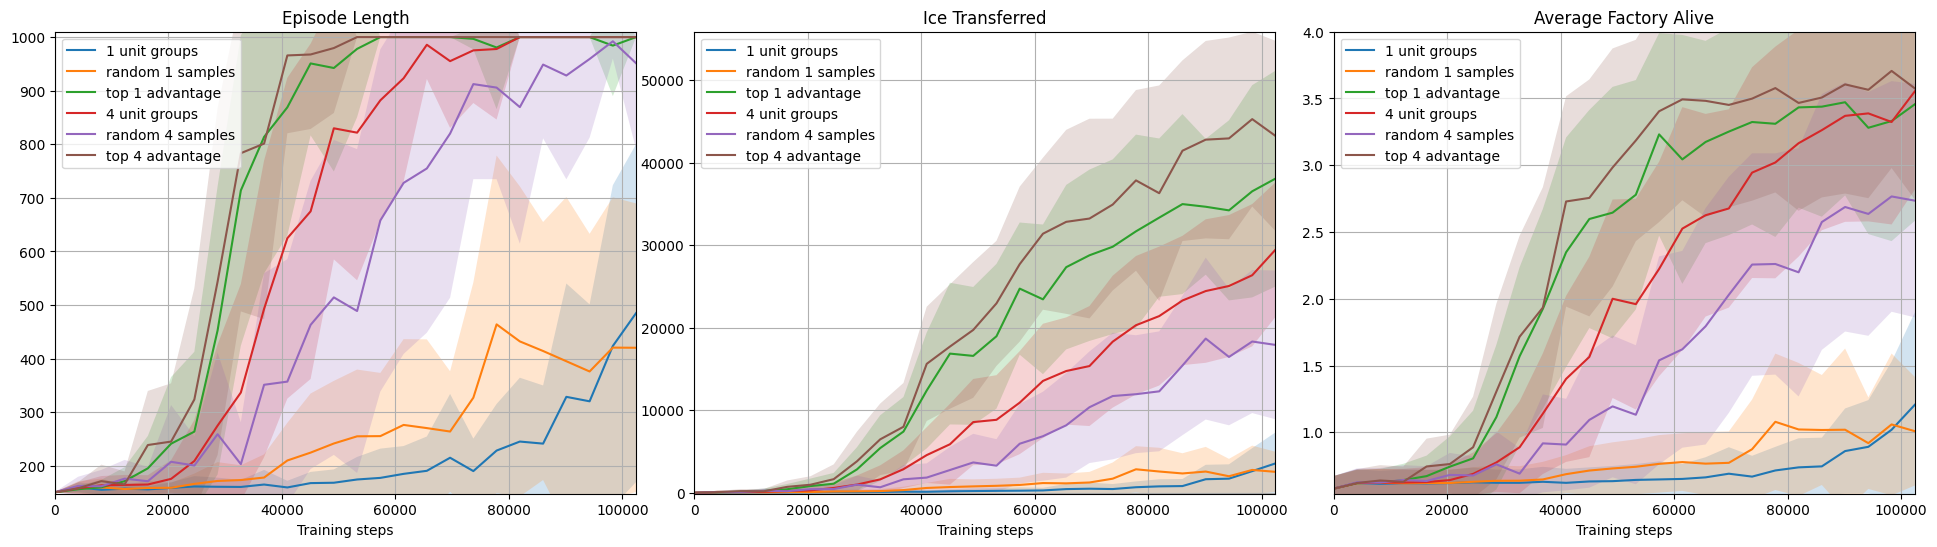
\includegraphics[width=0.95\linewidth]{images/results_hybrid/grouping_vs_tsr/combined.png}
    \captionsetup{justification=justified, singlelinecheck=false, width=1\linewidth, labelfont=bf} 
    \caption[]{Plot comparing random grouping, random sampling, and advantage-based sampling in terms of the length of the episodes, ice transferred by units, and number of active factories. Sampling by advantage outperforms both random grouping and random sampling, even if the advantage-based sampling contains fewer trajectories, suggesting greater importance of data quality than quantity.}
    \label{fig:hybrid_results/grouping_vs_tsr/combined}
\end{figure}

\begin{table}[ht]
    \footnotesize
    \renewcommand{\arraystretch}{1.2}%
    \begin{tabularx}{\textwidth}{|X|C{2.3cm}|C{2.3cm}|C{2.0cm}|C{2.0cm}|}
        \hline
\multicolumn{1}{|Y|}{\textbf{Group Name}} & \textbf{Final Ice Transferred} & \textbf{Final Episode Length} & \textbf{10\% of Episodes Finished by} & \textbf{95\% of Episodes Finished by} \\
        \hline
1 unit groups & 3,573 (3,753) & 485 (315) & 98,304 steps & - \\
random 1 samples & 2,550 (2,434) & 420 (269) & 77,824 steps & - \\
top 1 advantage & 38,072 (13,071) & \textbf{1,000 (0)} & 32,768 steps & 57,344 steps \\
4 unit groups & 29,459 (8,150) & \textbf{1,000 (0)} & 36,864 steps & 77,824 steps \\
random 4 samples & 17,927 (9,007) & 951 (160) & 45,056 steps & - \\
top 4 advantage & \textbf{43,246 (11,518)} & \textbf{1,000 (0)} & \textbf{28,672 steps} & \textbf{49,152 steps} \\
        \hline
    \end{tabularx}
    \medskip
    \captionsetup{justification=justified, singlelinecheck=false, width=1\linewidth, labelfont=bf} 
    \caption{Table comparing random grouping, random sampling, and advantage-based sampling. The metrics featured include the amount of ice transferred by units and the length of the episodes in the evaluation phase following the last training cycle. The table also contains the observed environment steps needed until the model reaches the maximum episode length in the specified percentage of evaluation environments. The advantage-based sampling managed to outperform the other variants in all metrics, even with fewer training examples, while the random sampling underperformed random grouping.}
    \label{tab:hybrid_results/grouping_vs_tsr/combined}
\end{table}


\subsection{Method Components}
\label{subsec:methodcomp}

\noindent Although the results obtained in \autoref{sec:trajectory-separation} seem impressive, it is \textbdd{challenging to identify} the specific factor that has led to such a substantial \textbdd{improvement in performance}. Based on our current understanding, the act of separating the trajectories leads to four notable enhancements in the training process. The process generates additional \textbdd{training examples} from the same environmental steps, thereby enhancing the model's ability to acquire broader policies at an accelerated rate through increased exploration. Another, perhaps the most noteworthy advantage, is the eradication of the \textbdd{reinforcement of undesirable behavior}. Such reinforcement could arise if one entity performs an action that results in a high advantage value while another entity behaves in a manner that is suboptimal for the team's success but doesn't get punished by enough negative advantage. In this case, the incorrect action would be reinforced alongside the positive action. By employing separate trajectories with \textbdd{localized rewards}, the occurrence of such events can be prevented. Our method also \textbdd{avoids calculating} advantage from steps where the \textbdd{original performing entity is no longer active}. If only a single trajectory were utilized, there would be no way to keep track of the status and reward of individual entities. Within highly dynamic environments, such as Lux, this phenomenon leads to a somewhat \textbdd{misleading calculation} due to the significant probability that the units and factories currently in existence will not persist until the conclusion of the episode. Consequently, it is \textbdd{impossible to determine} whether their actions in the present have truly contributed to \textbdd{any real advantage}. By keeping the rewards separate, we ensure that the entity receives credit for its immediate and observable efforts, both in the present and future. Lastly, separate trajectories result in separate \textbdd{advantage} calculations and separate \textbdd{critic value} outputs for all groups. Estimating the \textbdd{entire game state} in order to provide a final \textbdd{global value} is a significantly \textbdd{more complex} task for the model compared to predicting multiple values based on \textbdd{local observations}. Within this subsection, we examine the \textbdd{different components} of trajectory separation to determine which part has the greatest impact on enhancing performance.

\subsubsection{Inividual Components}
\label{subsec:individual-components}

\noindent Our initial hypothesis was that the most crucial components that needed to be separated were the \textbdd{reward}, \textbdd{terminal state} indication, \textbdd{critic value}, \textbdd{log probabilities}, and \textbdd{entropy} values. Therefore, we conducted a series of experiments where we systematically removed the separation of these components one by one. The purpose of these experiments was to observe the impact of each component's loss on the model's overall performance.

\bigskip

\noindent Both the \textbdd{reward} and \textbdd{critic} values are essential for the computation of the \textbdd{advantage}, an integral component of the Proximal Policy Optimization (\autoref{sec:ppo}) algorithm. Therefore, we decided to start with removing separation between these values. The results can be seen in \autoref{fig:hybrid_results/components/combined_rew} and \autoref{tab:hybrid_results/components/combined_rew}. The metrics for the \textttdb{"separate trajectories, global reward"} variant indicate that the utilization of separate trajectories with global rewards leads to a notable decrease in convergence speed, in comparison to separate trajectories with \textbdd{localized rewards}. This negative effect was expected since the absence of separated rewards hinders the model's ability to \textbdd{identify the specific actions} undertaken by the units and factories that led to the rewards received. Consequently, this issue aligns with the problem outlined in \autoref{par:global-rew}. In order to achieve efficient global advantage calculation, the critic head of the model must learn how to \textbdd{predict the performance of the entire team} rather than solely relying on predictions based on the local observations of individual entities. The decline in performance due to losing the ability to calculate \textbdd{critic value} predictions based on local information is further indicated by the \textttdb{"separate trajectories, global critic"} variant. The agents were able to sustain the operation of the factories for up to 1,000 steps in most environments, albeit at a slower pace, demonstrating how \textbdd{harder} it is for the model to work \textbdd{solely from global information}. Only when we remove both the \textbdd{critic values} and \textbdd{rewards} in test \textttdb{"separate trajectories, global advantage"} do we observe a reduction in performance to the level of a single global trajectory. A fully global \textbdd{advantage} calculation results in the \textbdd{same advantage value output for all entities}, meaning there is no way to differentiate between positive and negative actions under the same step, massively slowing down the training. Following this modification, the only difference in the policy loss between the entities is the \textbdd{probability ratios}, which fail to provide us any information about the desired direction and magnitude of policy updates. Due to the abovementioned factors, we believe that separate rewards hold significant importance. The impact of their effect is further examined in \autoref{subsubsec:rewardass}.

\bigskip

\noindent The outcomes following the elimination of the remaining separation components, namely the termination flags and the action probabilities, are observable in \autoref{fig:hybrid_results/components/combined_misc} and \autoref{tab:hybrid_results/components/combined_misc}. The fact that the performance remained consistent even after the removal of the separated \textbdd{terminal state flags} was unexpected and surprising to us. This group can be seen under the name \textttdb{"separate trajectories, global dones"}. Given that the trajectories are separated, and \textbdd{only currently active entities receive rewards}, indicating episode terminations prematurely at the destruction of an entity is somewhat \textbdd{redundant} since there will be no future rewards assigned to them that could skew the return calculation anyway. The act of indicating the inactivity of a group of agents is more logical in situations where the group has the potential to become active once again, particularly in cases where multiple entities are present within the same group. If all entities within the group are destroyed, but subsequently, a new entity is assigned, it is possible for the group to regain its activity. Whether stopping the future reward calculation between these two group states is beneficial is yet to be explored. The separation of \textbdd{distribution entropy values} does not appear to have any significance, as these values are ultimately combined into a single value to calculate the entropy loss regularization term. What massively degraded performance, however, was the removal of the \textbdd{separated log probabilities}. Through the aggregation of log probabilities, the gradients can \textbdd{propagate across} the action calculations of \textbdd{all entities}. Similarly to the combined advantage value, this global gradient propagation causes weight adjustments based on the whole team's performance, making it impossible to separate individual contributions. This observation shows the necessity of utilizing separate action probabilities in order to achieve optimal training.

\begin{figure}[htbp]
    \centering
    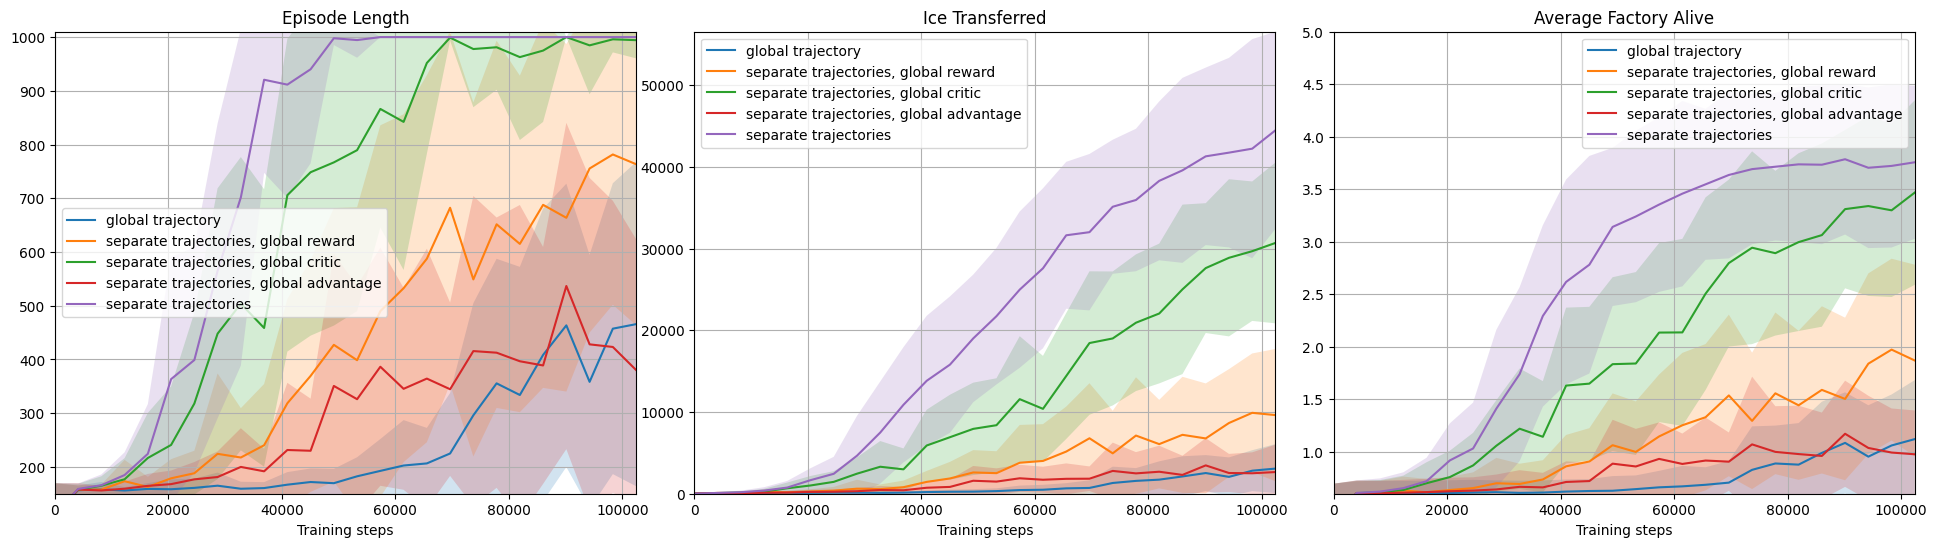
\includegraphics[width=0.95\linewidth]{images/results_hybrid/components/combined_rew.png}
    \captionsetup{justification=justified, singlelinecheck=false, width=1\linewidth, labelfont=bf} 
    \caption[]{Plot comparing the removal of separated components relevant to the advantage calculation in terms of the length of the episodes, ice transferred by units, and number of active factories. In addition to the test variants, the global and completely separate trajectory variants are also present. The separated reward plays a significant role but doesn't account for the whole performance boost. Removing separated critic value predictions and separated rewards together results in a similar performance to a single global trajectory.}
    \label{fig:hybrid_results/components/combined_rew}
\end{figure}

\begin{table}[ht]
    \footnotesize
    \renewcommand{\arraystretch}{1.2}%
    \begin{tabularx}{\textwidth}{|X|C{2.3cm}|C{2.3cm}|C{2.0cm}|C{2.0cm}|}
        \hline
\multicolumn{1}{|Y|}{\textbf{Group Name}} & \textbf{Final Ice Transferred} & \textbf{Final Episode Length} & \textbf{10\% of Episodes Finished by} & \textbf{95\% of Episodes Finished by} \\
        \hline
global trajectory & 3,066 (2,996) & 466 (302) & 102,400 steps & - \\
separate trajectories, global reward & 9,614 (8,094) & 763 (300) & 53,248 steps & - \\
separate trajectories, global critic & 30,687 (9,844) & 994 (34) & 40,960 steps & 69,632 steps \\
separate trajectories, global advantage & 2,643 (3,353) & 380 (244) & 73,728 steps & - \\
separate trajectories & \textbf{44,472 (12,065)} & \textbf{1,000 (0)} & \textbf{28,672 steps} & \textbf{49,152 steps} \\
        \hline
    \end{tabularx}
    \medskip
    \captionsetup{justification=justified, singlelinecheck=false, width=1\linewidth, labelfont=bf} 
    \caption{Table comparing the removal of separated components relevant to the advantage calculation. The metrics featured include the amount of ice transferred by units and the length of the episodes in the evaluation phase following the last training cycle. The table also contains the observed environment steps needed until the model reaches the maximum episode length in the specified percentage of evaluation environments. In addition to the test variants, the global and completely separate trajectory variants are also present. Removing the separation of rewards and critic values caused a significant performance decrease. Reward appears to be the most important component.}
    \label{tab:hybrid_results/components/combined_rew}
\end{table}

\begin{figure}[htbp]
    \centering
    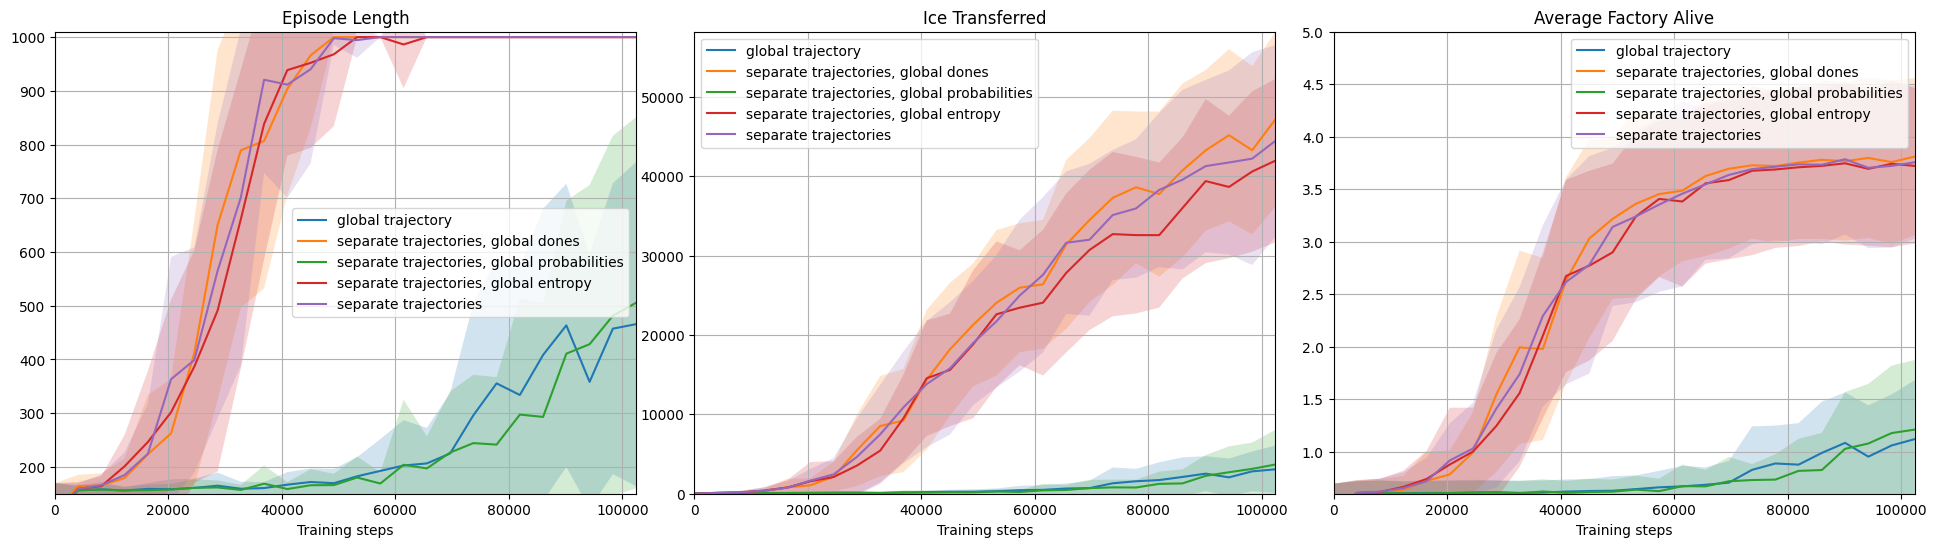
\includegraphics[width=0.95\linewidth]{images/results_hybrid/components/combined_misc.png}
    \captionsetup{justification=justified, singlelinecheck=false, width=1\linewidth, labelfont=bf} 
    \caption[]{Plot comparing the removal of other separated components in terms of the length of the episodes, ice transferred by units, and number of active factories. In addition to the test variants, the global and completely separate trajectory variants are also present. Aggregating the action probabilities globally degrades the model's performance to the level of a single global trajectory.}
    \label{fig:hybrid_results/components/combined_misc}
\end{figure}

\begin{table}[ht]
    \footnotesize
    \renewcommand{\arraystretch}{1.2}%
    \begin{tabularx}{\textwidth}{|X|C{2.3cm}|C{2.3cm}|C{2.0cm}|C{2.0cm}|}
        \hline
\multicolumn{1}{|Y|}{\textbf{Group Name}} & \textbf{Final Ice Transferred} & \textbf{Final Episode Length} & \textbf{10\% of Episodes Finished by} & \textbf{95\% of Episodes Finished by} \\
        \hline
global trajectory & 3,066 (2,996) & 466 (302) & 102,400 steps & - \\
separate trajectories, global dones & \textbf{47,201 (11,018)} & \textbf{1,000 (0)} & \textbf{28,672 steps} & \textbf{49,152 steps} \\
separate trajectories, global probabilities & 3,673 (4,372) & 506 (345) & 98,304 steps & - \\
separate trajectories, global entropy & 41,970 (10,305) & \textbf{1,000 (0)} & \textbf{28,672 steps} & 53,248 steps \\
separate trajectories & 44,472 (12,065) & \textbf{1,000 (0)} & \textbf{28,672 steps} & \textbf{49,152 steps} \\
        \hline
    \end{tabularx}
    \medskip
    \captionsetup{justification=justified, singlelinecheck=false, width=1\linewidth, labelfont=bf} 
    \caption{Table comparing the removal of other separated components. The metrics featured include the amount of ice transferred by units and the length of the episodes in the evaluation phase following the last training cycle. The table also contains the observed environment steps needed until the model reaches the maximum episode length in the specified percentage of evaluation environments. In addition to the test variants, the global and completely separate trajectory variants are also present. The table demonstrates the importance of separate action probabilities in order to limit the gradient flow to only relevant parts of the network during training.}
    \label{tab:hybrid_results/components/combined_misc}
\end{table}

\subsubsection{Reward Assignment}
\label{subsubsec:rewardass}

\noindent Based on the findings reported in \autoref{subsec:individual-components}, which indicated a significant impact of reward separation on performance, our objective was to investigate the importance of \textbdd{localized rewards}. To achieve this, we conducted an experiment combining the local, separated reward with the aggregated \textbdd{global reward}. Agents were allocated different percentages of their own rewards, specifically 0\%, 50\%, 75\%, and 100\% of their own rewards, with the remaining percentages being made up by the global reward. As evident from the data presented in \autoref{fig:hybrid_results/reward_assignment/combined} and \autoref{tab:hybrid_results/reward_assignment/combined}, the variant with completely separate reward values demonstrates superior performance compared to the other variants. Utilizing 25\% of the global rewards appears to result in convergence to an episode length of 1,000 at approximately the same step. Nevertheless, it gets outperformed in the \textbdd{ice transferred} and \textbdd{average factory alive} metrics by the completely separate variant. The variant that receives 50\% global rewards achieves the maximum episode length on average, whereas the variant that solely relies on global rewards fails to converge even after 100,000 steps. This experiment provides additional evidence to support the significance of localized rewards.

\begin{figure}[htbp]
    \centering
    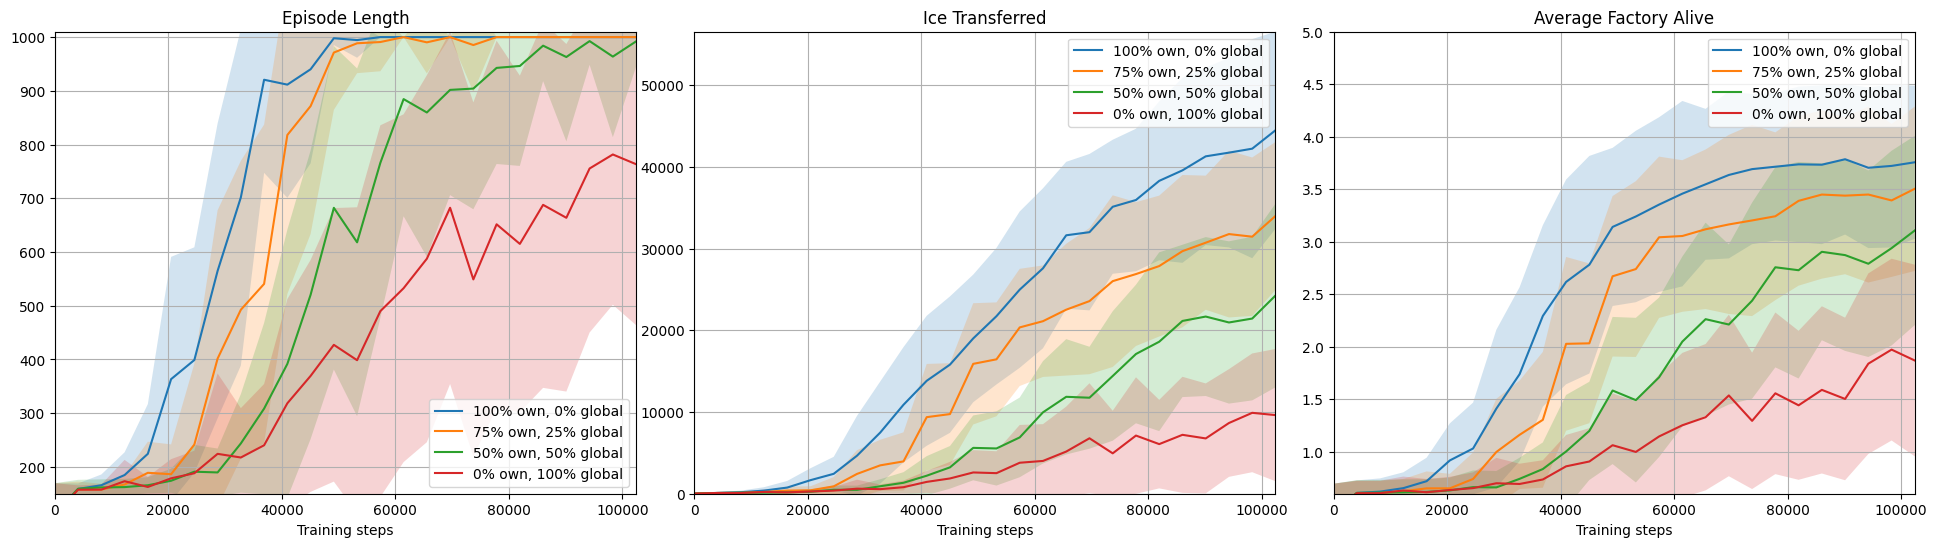
\includegraphics[width=0.95\linewidth]{images/results_hybrid/reward_assignment/combined.png}
    \captionsetup{justification=justified, singlelinecheck=false, width=1\linewidth, labelfont=bf} 
    \caption[]{Plot comparing the performance of different percentages of global and local rewards in terms of the length of the episodes, ice transferred by units, and number of active factories. In addition to the test variants, the global and completely separate trajectory variants are also present. Mixing in global rewards seems to hinder performance.}
    \label{fig:hybrid_results/reward_assignment/combined}
\end{figure}

\begin{table}[ht]
    \footnotesize
    \renewcommand{\arraystretch}{1.2}%
    \begin{tabularx}{\textwidth}{|X|C{2.3cm}|C{2.3cm}|C{2.0cm}|C{2.0cm}|}
        \hline
\multicolumn{1}{|Y|}{\textbf{Group Name}} & \textbf{Final Ice Transferred} & \textbf{Final Episode Length} & \textbf{10\% of Episodes Finished by} & \textbf{95\% of Episodes Finished by} \\
        \hline
100\% own, 0\% global & \textbf{44,472 (12,065)} & \textbf{1,000 (0)} & \textbf{28,672 steps} & \textbf{49,152 steps} \\
75\% own, 25\% global & 33,985 (9,059) & \textbf{1,000 (0)} & \textbf{28,672 steps} & 57,344 steps \\
50\% own, 50\% global & 24,244 (11,238) & 992 (47) & 45,056 steps & 94,208 steps \\
0\% own, 100\% global & 9,614 (8,094) & 763 (300) & 53,248 steps & - \\
        \hline
    \end{tabularx}
    \medskip
    \captionsetup{justification=justified, singlelinecheck=false, width=1\linewidth, labelfont=bf} 
    \caption{Table comparing the performance of different global and local reward percentages. The metrics featured include the amount of ice transferred by units and the length of the episodes in the evaluation phase following the last training cycle. The table also contains the observed environment steps needed until the model reaches the maximum episode length in the specified percentage of evaluation environments. In addition to the test variants, the global and completely separate trajectory variants are also present.}
    \label{tab:hybrid_results/reward_assignment/combined}
\end{table}


\subsection{Comparison with Other Works}
\label{subsec:comparison}

\noindent As previously stated in this section, the training objectives in the experiments demonstrating \textbdd{trajectory separation} (\autoref{sec:trajectory-separation}) were focused on achieving the \textbdd{maximum episode length}, which can be accomplished by keeping at least one factory alive from both players. Factories have a \textbdd{lichen watering} action (\autoref{sec:wincondition}), which is used to determine the winner if both players successfully maintain their factories until the maximum duration of the episode. In the previous experiments, we masked out (\autoref{subsec:actions}) this watering action in order to achieve faster convergence. This decision was made since watering can \textbdd{reduce the potential lifespan of a factory}. Consequently, in order to conduct a comparative analysis between our approach and state-of-the-art solutions, it was necessary to enable lichen watering. As a result, we proceeded to train a \textbdd{slightly different} version of our model. We used trajectory separation without any kind of grouping rule (\autoref{subsec:grouping}) or trajectory sample reduction (\autoref{subsec:tsr}). Given that the other solutions gave rewards for growing lichen, we made adjustments to the reward functions so that the factories received \textbdd{rewards proportional to the number of lichen tiles} present on the board at the end of the episode. Lichen can only be grown on rubbleless tiles; thus, we also rewarded units after \textbdd{clearing away rubble} next to factories and lichen tiles. We measured how long it took for the modified model to learn how to keep the factories alive up to the maximum episode length. The performance of the modified model compared to the original can be observed in \autoref{fig:hybrid_results/lichen_vs_ts/combined} and \autoref{tab:hybrid_results/lichen_vs_ts/combined}. Even though enabling and rewarding the watering action caused a slight decrease in performance, the model still managed to learn how to transport sufficient ice to factories. It also learned how to successfully grow lichen, as can be seen in \autoref{fig:hybrid_results/lichen/combined}.

\begin{figure}[htbp]
    \centering
    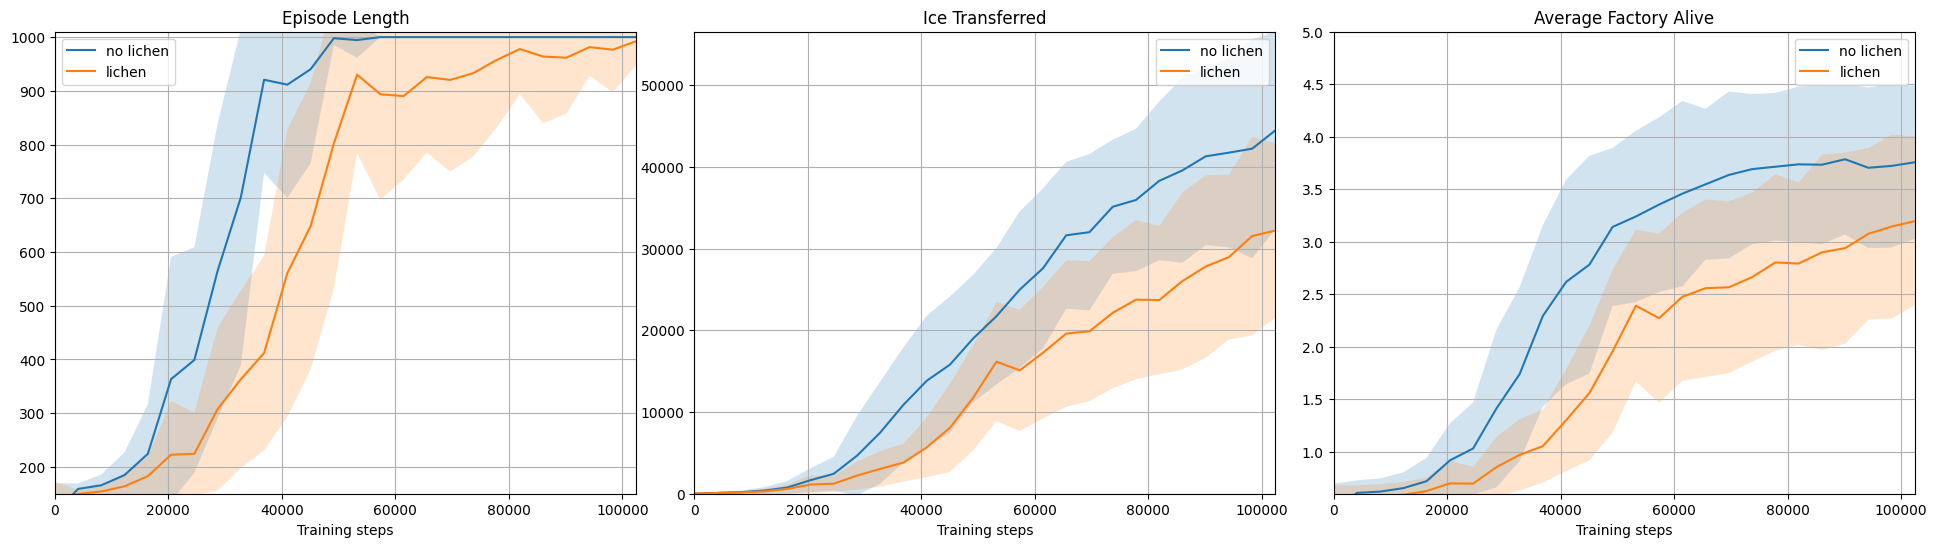
\includegraphics[width=0.95\linewidth]{images/results_hybrid/lichen_vs_ts/combined.png}
    \captionsetup{justification=justified, singlelinecheck=false, width=1\linewidth, labelfont=bf} 
    \caption[]{Plot comparing the performance of the new lichen-enabled model to the original in terms of the length of the episodes, ice transferred by units, and number of active factories. While lichen watering degrades performance, the goal of reaching the maximum episode length is still achieved at the end of the observed step range.}
    \label{fig:hybrid_results/lichen_vs_ts/combined}
\end{figure}

\begin{table}[ht]
    \footnotesize
    \renewcommand{\arraystretch}{1.2}%
    \begin{tabularx}{\textwidth}{|X|C{2.3cm}|C{2.3cm}|C{2.0cm}|C{2.0cm}|}
        \hline
\multicolumn{1}{|Y|}{\textbf{Group Name}} & \textbf{Final Ice Transferred} & \textbf{Final Episode Length} & \textbf{10\% of Episodes Finished by} & \textbf{95\% of Episodes Finished by} \\
        \hline
no lichen & \textbf{44,472 (12,065)} & \textbf{1,000 (0)} & \textbf{28,672 steps} & \textbf{49,152 steps} \\
lichen & 32,199 (10,670) & 992 (45) & 40,960 steps & 102,400 steps \\
        \hline
    \end{tabularx}
    \medskip
    \captionsetup{justification=justified, singlelinecheck=false, width=1\linewidth, labelfont=bf} 
    \caption{Table comparing the performance of the new lichen-enabled model to the original. The metrics featured include the amount of ice transferred by units and the length of the episodes in the evaluation phase following the last training cycle. The table also contains the observed environment steps needed until the model reaches the maximum episode length in the specified percentage of evaluation environments. In addition to the test variants, the global and completely separate trajectory variants are also present. The lichen-enabled variant managed to reach the desired 95\% of completed episodes by the end of the observed step range.}
    \label{tab:hybrid_results/lichen_vs_ts/combined}
\end{table}

\begin{figure}[htbp]
    \centering
    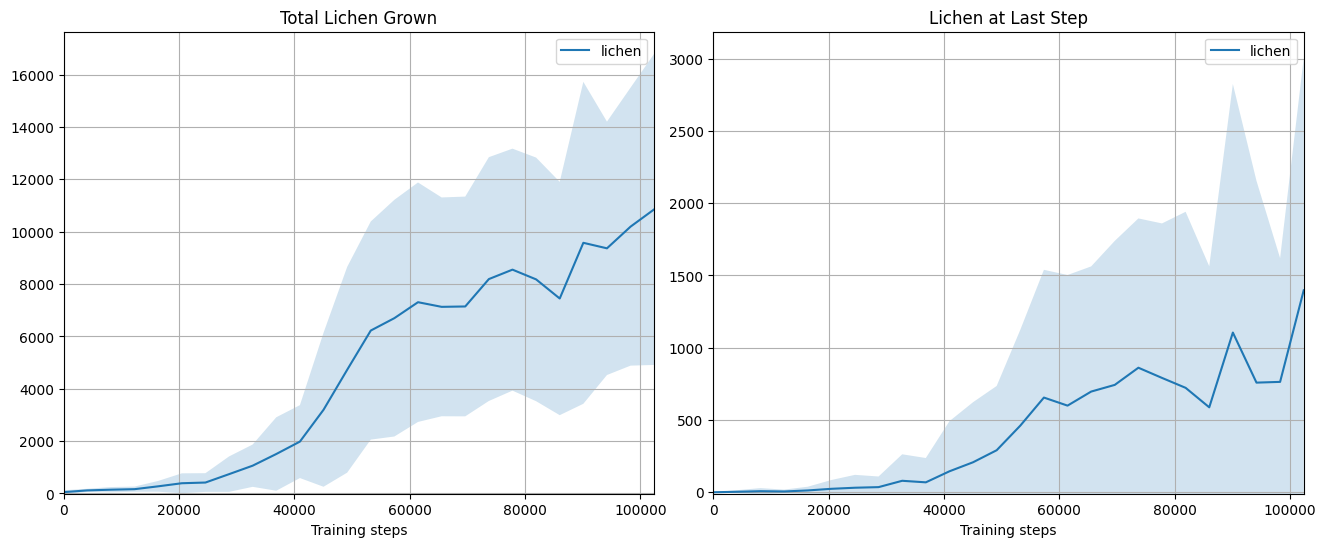
\includegraphics[width=0.95\linewidth]{images/results_hybrid/lichen/combined.png}
    \captionsetup{justification=justified, singlelinecheck=false, width=1\linewidth, labelfont=bf} 
    \caption[]{Plot showcasing the amount of total lichen grown and the amount of lichen at the end of the episodes. In addition to learning how to reach the maximum episode length (\autoref{fig:hybrid_results/lichen_vs_ts/combined}), the agent demonstrated the ability to solve a secondary task, as shown by the ascending lines.}
    \label{fig:hybrid_results/lichen/combined}
\end{figure}

\bigskip

\noindent We wanted to compare our solution to the \textbdd{top-performing submissions} in the Lux AI competition. The basis of our comparison is how long it took for the different models to reach a state where they could \textbdd{keep the factories alive} until the maximum episode length \textbdd{in most environments}. In our case, this goal was 95\% of episodes. Unfortunately, the leaderboards were predominantly controlled by \textbdd{rule-based methods}, resulting in very few RL-based submissions that could be used for a comparative analysis. Many refrained from sharing their work, and in lots of cases where they did share it, their trained models or training metrics were \textbdd{not made publicly available}. The only somewhat reliable source we could find was \textbdd{FLG's submission} (\cite{ferdinand}), which was somewhat similar to the pixel-to-pixel architecture we started with. Their training objective during the initial \textbdd{set-up phase} was comparable to ours, which aimed to teach the agent fundamental aspects of the game, such as gathering resources. The duration of their training in terms of time and steps was outlined; however, we are not sure what their stopping criteria were. Consequently, for the purpose of our comparison, we will assume that the stopping criterion used in the referenced submission was identical to our own. In addition, we included a \textbdd{baseline solution} provided by the competition organizers (\cite{luxai_s2-baseline-source}). The comparison can be seen in \autoref{tab:other-work-comparisons}. Our approach massively outperformed both the baseline and the FLG's submission in every single one of our metrics. We managed to reach the maximum episode length in 95\% of the environments by step 102,400. In comparison, the baseline model required 1.4 million steps to reach the same milestone, while the submission of FLG was trained for 65 million steps. Given that we utilized a larger value for the hyperparameter \textbdd{number of epochs} compared to the baseline, resulting in faster training, we believed it was necessary to account for this difference in our comparison. Having said that, our approach is still 5 times more efficient in terms of weight updates needed. Our approach also yielded significantly reduced model sizes, with a mere 200 thousand trainable parameters, as opposed to 451 thousand and 6.08 million, respectively. We also compared the training times, although it should be noted that the resources used for training the other two solutions remain undisclosed, potentially introducing a bias to the presented values.

\bigskip

% time it took for ours to reach 102k steps:
% 2.143 h
% 2.113 h
% 1.999 h
% avg: 2.085 h

\begin{table}[htbp]
    \footnotesize
    \renewcommand{\arraystretch}{1.2}%
    \begin{threeparttable}
        \begin{tabularx}{\linewidth}{|X|C{2.0cm}|C{2.0cm}|C{2.0cm}|C{2.0cm}|}
            \hline
            \textbf{Solution} & \textbf{Parameters}  & \textbf{Training time} & \textbf{Environment Steps} & \textbf{Training Epochs} \\
            \hline
            Trajectory Separated Hybrid Approach & \textbf{200K} & \textbf{2 hours} & \textbf{102K} & \textbf{250} \\
            Baseline Solution (\cite{luxai_s2-baseline-source}) & 451K & 2 days & 1.4M & 1364 \\
            Best RL Submission (\cite{ferdinand}) & 6.08M & 2 days\tnote{*} & 65M\tnote{*} & ?\tnote{**} \\
            \hline
        \end{tabularx}
        \begin{tablenotes}
            \item[*] exact stopping criterion is not known, only the number of steps the model was trained on and the time of training.
            \item[**] \textbdd{number of epochs} hyperparameter not provided.
        \end{tablenotes}
        \captionsetup{justification=justified, singlelinecheck=false, width=1\linewidth, labelfont=bf} 
        \caption{Table containing the comparison of our work with other implementations. We included the best-performing reinforcement learning submission of the Lux AI competition and a baseline repository provided by the organizers. Our method outperforms both of them in terms of both training time and observed environment steps needed to reach the designated goal. The table also shows a significant difference in model sizes.}
        \label{tab:other-work-comparisons}
    \end{threeparttable}
\end{table}


\subsection{Model Ablation Study}
\label{subsec:ablation}

\noindent Through the utilization of \textbdd{trajectory separation} (\autoref{sec:trajectory-separation}), we achieved a significant acceleration in the training process of our model. However, as previously discussed in \autoref{sec:monolithic-approach} and \autoref{sec:hybrid-approach}, many additional components played an important role in achieving the level of performance described, with \textbdd{certain components being absolutely indispensable}. In this subsection, we performed an ablation study on the key methods employed to demonstrate the various factors that can impact reinforcement learning and the potential pitfalls that can arise.

\subsubsection{Weight Initialization}

\noindent The proper initialization of weights plays a crucial role, particularly in the application of algorithms such as Proximal Policy Optimization (\autoref{sec:ppo}). We have provided an overview of the weight initialization structure of our model in \autoref{subsec:weight-scaling} and will delve into this issue further in \autoref{ch:disc-init-is-all-you-need}. In this study, we aim to illustrate the impact of incorrect initialization on the convergence of our trajectory-separated \textbdd{hybrid} (\autoref{sec:hybrid-approach}) model. The study involved the examination of two components: the weight initialization \textbdd{scaling} in the \textbdd{output layers} and an \textbdd{additional scaling} applied to \textbdd{all the weights} after initialization, referred to as \textbdd{extra scaling}. We tested removing the extra scaling from the hidden layers (\textttdb{"no extra hidden layer scaling"}) as well as from all layers (\textttdb{"no extra scaling"}). We also conducted experiments to evaluate the effects of removing any kind of scaling from the actor output layers (\textttdb{"no actor scaling"}), the critic value output layers (\textttdb{"no value scaling"}), and all output layers (\textttdb{"no scaling"}). As presented in \autoref{fig:hybrid_results/ablation_study/combined_init} and \autoref{tab:hybrid_results/ablation_study/combined_init}, the \textbdd{removal of any} weight initialization component leads to \textbdd{deterioration of performance}. Eliminating all \textbdd{weight-downscaling techniques} renders the model incapable of any kind of learning. The main problem with large weights is their \textbdd{effect on the initial policies}. A network that exhibits a high degree of bias may not assign \textbdd{equal probabilities} to all possible actions, resulting in a decrease in the \textbdd{exploration} of different actions and a slower rate of learning. This biased network can sometimes lead to \textbdd{policy collapse}, as observed with variant \textttdb{"no actor scaling"}. Interestingly, removing the critic value output's scaling causes even larger performance degradation because the early parts of the training must be spent on training the value network to overcome its \textbdd{inherent bias}. As a result, the predicted advantage values, which are essential for the PPO algorithm, will be inaccurate.

\begin{figure}[htbp]
    \centering
    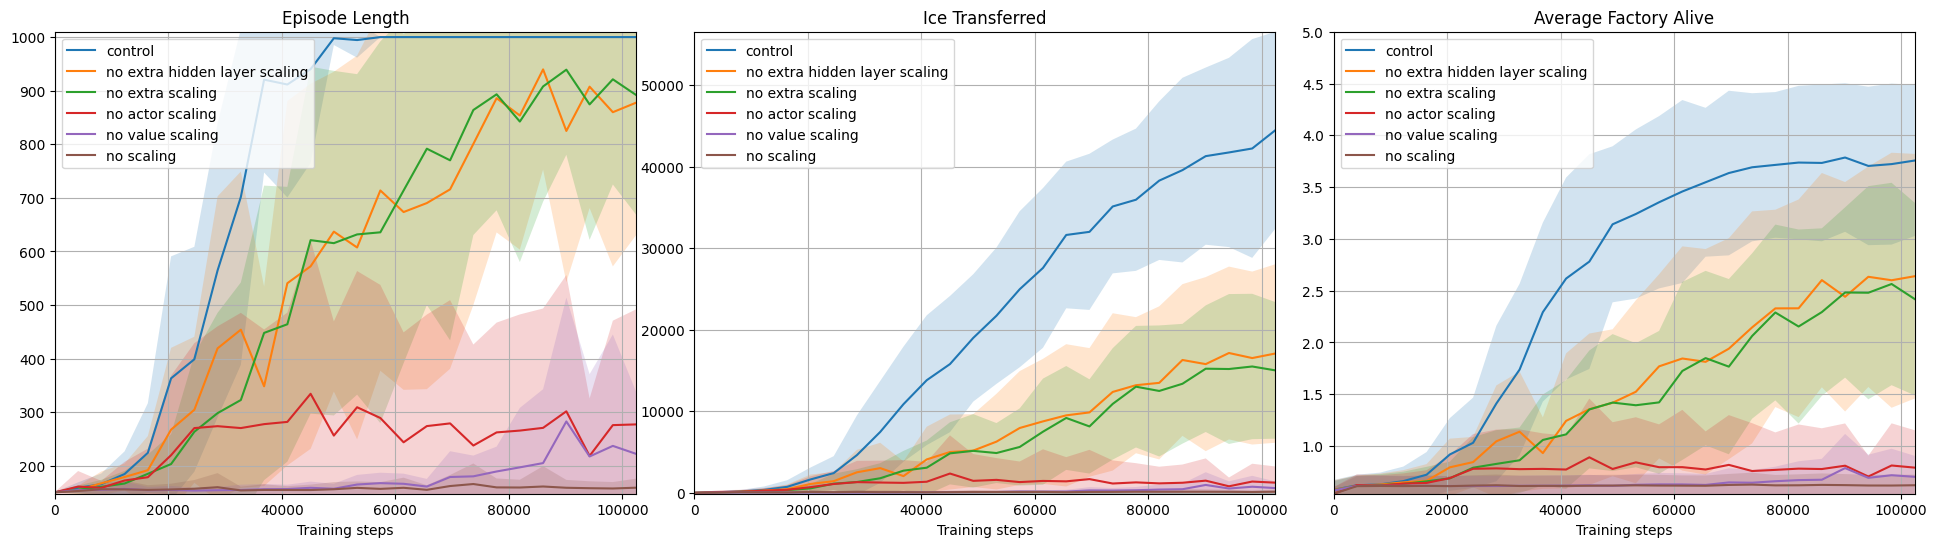
\includegraphics[width=0.95\linewidth]{images/results_hybrid/ablation_study/combined_init.png}
    \captionsetup{justification=justified, singlelinecheck=false, width=1\linewidth, labelfont=bf} 
    \caption[]{Plot showcasing the difference in performance weight magnitudes can cause in terms of the length of the episodes, ice transferred by units, and number of active factories. Removing any kind of weight downscaling caused a significant performance decrease. Not scaling down the weights of the output layer at all makes training impossible for the model.}
    \label{fig:hybrid_results/ablation_study/combined_init}
\end{figure}

\begin{table}[ht]
    \footnotesize
    \renewcommand{\arraystretch}{1.2}%
    \begin{tabularx}{\textwidth}{|X|C{2.3cm}|C{2.3cm}|C{2.0cm}|C{2.0cm}|}
        \hline
\multicolumn{1}{|Y|}{\textbf{Group Name}} & \textbf{Final Ice Transferred} & \textbf{Final Episode Length} & \textbf{10\% of Episodes Finished by} & \textbf{95\% of Episodes Finished by} \\
        \hline
control & \textbf{44,472 (12,065)} & \textbf{1,000 (0)} & \textbf{28,672 steps} & \textbf{49,152 steps} \\
no extra hidden layer scaling & 17,093 (10,944) & 878 (247) & 32,768 steps & - \\
no extra scaling & 15,019 (8,371) & 892 (223) & 36,864 steps & - \\
no actor scaling & 1,255 (1,986) & 277 (215) & 45,056 steps & - \\
no value scaling & 591 (811) & 222 (116) & - & - \\
no scaling & 145 (257) & 159 (17) & - & - \\
        \hline
    \end{tabularx}
    \medskip
    \captionsetup{justification=justified, singlelinecheck=false, width=1\linewidth, labelfont=bf} 
    \caption[]{Table showcasing the difference in performance weight magnitudes can cause. The metrics featured include the amount of ice transferred by units and the length of the episodes in the evaluation phase following the last training cycle. The table also contains the observed environment steps needed until the model reaches the maximum episode length in the specified percentage of evaluation environments. The table clearly shows the decline in performance caused by taking away the weight scalings one by one. None of the studied variants managed to learn how to keep the factories alive until the maximum episode length in most environments.}
    \label{tab:hybrid_results/ablation_study/combined_init}
\end{table}

\subsubsection{Removing Heuristics}

\noindent Our implementation of \textbdd{action masking} (\autoref{subsec:mono-actions}) and \textbdd{factory placement} (\autoref{subsec:heur-bidding-factory}) introduces a great level of \textbdd{heuristics} into the system. Action masking decreases the action space, resulting in faster convergence. Additionally, the strategic placement of factories in close proximity to ice tiles simplifies the environment. Both of these factors play a crucial role, as can be observed in \autoref{fig:hybrid_results/ablation_study/combined_heuristics} and \autoref{tab:hybrid_results/ablation_study/combined_heuristics}. Without the implementation of action masking, the model is presented with an \textbdd{excessive number} of potential combinations in its \textbdd{action space}, leading to an inability to learn an optimal policy. Consequently, there was no significant increase observed in the \textbdd{episode length} metric throughout the entire training period. By setting the factory placement to random, the agents can still learn how to transport ice to factories. However, due to the \textbdd{varying distances} of ice tiles from factories in each episode, the units are \textbdd{unable to learn} how to keep the factories alive within the observed step range.

\begin{figure}[htbp]
    \centering
    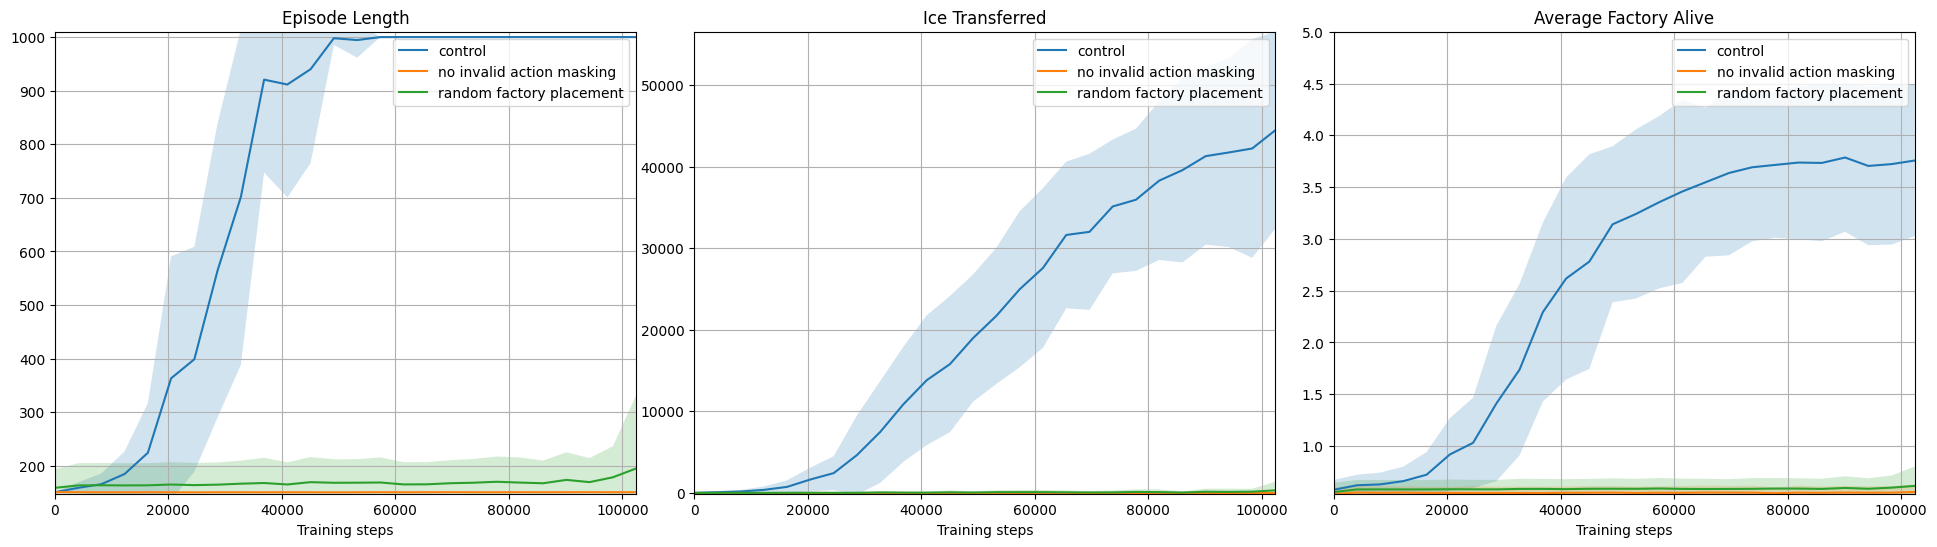
\includegraphics[width=0.95\linewidth]{images/results_hybrid/ablation_study/combined_heuristics.png}
    \captionsetup{justification=justified, singlelinecheck=false, width=1\linewidth, labelfont=bf} 
    \caption[]{Plot showcasing the difference in performance that removing heuristics causes in terms of the length of the episodes, ice transferred by units, and number of active factories. The elimination of action masking renders training infeasible within the specified step range that we have presented. In addition, the placement of factories at random locations introduces complexity to the environment, resulting in a significant decline in performance.}
    \label{fig:hybrid_results/ablation_study/combined_heuristics}
\end{figure}

\begin{table}[ht]
    \footnotesize
    \renewcommand{\arraystretch}{1.2}%
    \begin{tabularx}{\textwidth}{|X|C{2.3cm}|C{2.3cm}|C{2.0cm}|C{2.0cm}|}
        \hline
\multicolumn{1}{|Y|}{\textbf{Group Name}} & \textbf{Final Ice Transferred} & \textbf{Final Episode Length} & \textbf{10\% of Episodes Finished by} & \textbf{95\% of Episodes Finished by} \\
        \hline
control & \textbf{44,472 (12,065)} & \textbf{1,000 (0)} & \textbf{28,672 steps} & \textbf{49,152 steps} \\
no invalid action masking & 0 (0) & 151 (0) & - & - \\
random factory placement & 316 (1,055) & 195 (137) & - & - \\
        \hline
    \end{tabularx}
    \medskip
    \captionsetup{justification=justified, singlelinecheck=false, width=1\linewidth, labelfont=bf} 
    \caption[]{Table showcasing the difference in performance that removing heuristics causes. The metrics featured include the amount of ice transferred by units and the length of the episodes in the evaluation phase following the last training cycle. The table also contains the observed environment steps needed until the model reaches the maximum episode length in the specified percentage of evaluation environments. Without action masking, the units were unable to transfer any ice to factories. Random factory placement still allowed the units to learn that mining and transferring ice are advantageous, but they could not perform said actions optimally.}
    \label{tab:hybrid_results/ablation_study/combined_heuristics}
\end{table}

\subsubsection{Network Regularization}

\noindent In our network, we incorporated two crucial regularization components: \textbdd{batch normalization} (\autoref{subsec:batchnorm}) and \textbdd{spectral norm} (\autoref{subsec:spectralnorm}). In the following experiment, we tested the necessity of employing both regularization methods. As can be seen in \autoref{fig:hybrid_results/ablation_study/combined_net} and \autoref{tab:hybrid_results/ablation_study/combined_net}, it is apparent that the inclusion of \textbdd{some form of regularization is essential}. Removing batch normalization resulted in our model's inability to learn how to reach the maximum episode length within the observed step range. Interestingly, eliminating the spectral norm by itself did not significantly affect performance. Nevertheless, in the \textbdd{absence of batch normalization}, the \textbdd{performance deteriorated} even further when the spectral norm was removed. This observation suggests that the simultaneous use of both regularization methods may not be necessary. However, including \textbdd{at least one of them is crucial}, preferably batch normalization.

\begin{figure}[htbp]
    \centering
    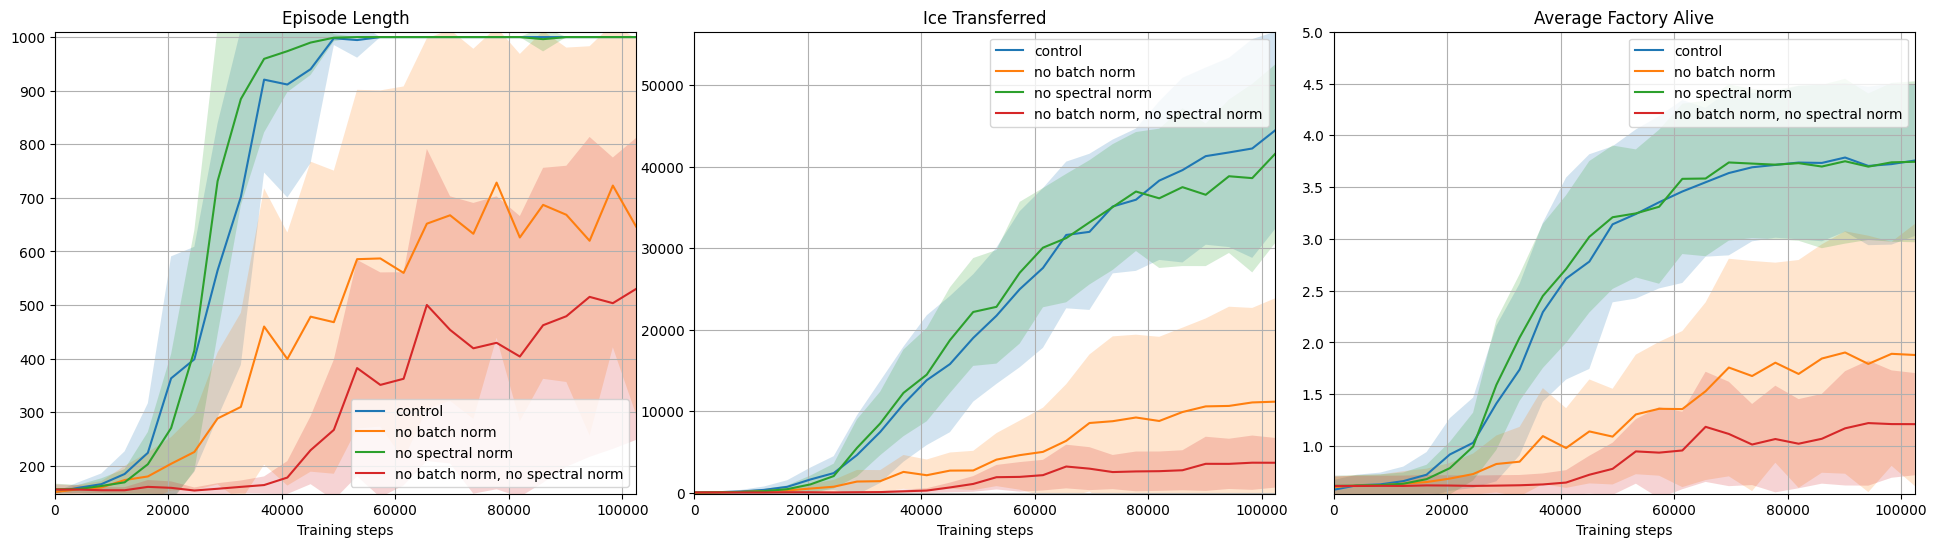
\includegraphics[width=0.95\linewidth]{images/results_hybrid/ablation_study/combined_net.png}
    \captionsetup{justification=justified, singlelinecheck=false, width=1\linewidth, labelfont=bf} 
    \caption[]{Plot showcasing the difference in performance that removing regularization from our network causes in terms of the length of the episodes, ice transferred by units, and number of active factories. It is clearly visible that batch normalization is the most important regularization component. However, if there is no batch normalization utilized in the network, the presence of spectral norm can help mitigate the need for regularization. Removing batch normalization appears to also cause high variance in the observed metrics.}
    \label{fig:hybrid_results/ablation_study/combined_net}
\end{figure}

\begin{table}[ht]
    \footnotesize
    \renewcommand{\arraystretch}{1.2}%
    \begin{tabularx}{\textwidth}{|X|C{2.3cm}|C{2.3cm}|C{2.0cm}|C{2.0cm}|}
        \hline
\multicolumn{1}{|Y|}{\textbf{Group Name}} & \textbf{Final Ice Transferred} & \textbf{Final Episode Length} & \textbf{10\% of Episodes Finished by} & \textbf{95\% of Episodes Finished by} \\
        \hline
control & \textbf{44,472 (12,065)} & \textbf{1,000 (0)} & \textbf{28,672 steps} & 49,152 steps \\
no batch norm & 11,184 (12,688) & 646 (351) & 53,248 steps & - \\
no spectral norm & 41,611 (10,938) & \textbf{1,000 (0)} & \textbf{28,672 steps} & \textbf{45,056 steps} \\
no batch norm, no spectral norm & 3,696 (3,039) & 530 (282) & 65,536 steps & - \\
        \hline
    \end{tabularx}
    \medskip
    \captionsetup{justification=justified, singlelinecheck=false, width=1\linewidth, labelfont=bf} 
    \caption[]{Table showcasing the difference in performance that removing regularization from our network causes. The metrics featured include the amount of ice transferred by units and the length of the episodes in the evaluation phase following the last training cycle. The table also contains the observed environment steps needed until the model reaches the maximum episode length in the specified percentage of evaluation environments. Removing batch normalization decreases the model's performance significantly, making it unable to learn how to reach the maximum episode length in all environments. Removing spectral norms further degrades performance.}
    \label{tab:hybrid_results/ablation_study/combined_net}
\end{table}

\cleardoublepage

\chapter{Discussion}
\label{ch:disc}

\noindent In the results sections, we presented extensive charts, data, and convergence metrics, offering a \textbdd{data-driven analysis} of the limitations in multi-agent reinforcement learning and potential solutions. However, our discussion chapter aims to provide a \textbdd{broader perspective} on our research journey, encompassing pivotal transitions and stages, along with novel insights and challenges encountered. We wrap up each section with concise \textbdd{recommendations for constructing robust systems} and cautionary notes on \textbdd{practices to avoid}.

\begin{itemize}

\item \autoref{ch:disc-diverse-domains} examines the \textbdd{adaptability of RL algorithms} across tasks and their effectiveness in multi-agent settings.
\item \autoref{ch:disc-dictatorship-failure} analyzes the \textbdd{inability of dictatorial approaches to converge} in complex, dynamic environments where global views may not suffice.
\item \autoref{ch:disc-beyond-one-mind} investigates the \textbdd{transition to a multi-scale environment} overview and its implications on individuality and agent performance.
\item \autoref{ch:disc-init-is-all-you-need} discusses the critical \textbdd{role of initialization and regularization} in deep RL, highlighting their impact on convergence and avoidance of local optima.
\item \autoref{ch:disc-paying-for-performance} explores the \textbdd{trade-offs of model complexity and training time}, particularly in the context of Lux AI competitions where submissions often prioritize deep neural nets without sufficient consideration of problem-solving approaches.
\item \autoref{ch:disc-singular-to-spectrum} analyzes the \textbdd{transferability of learned behaviors} in MARL systems, focusing on the dynamics of alignment and reward shaping and their implications on agent performance.

\end{itemize}

\section{Diverse Domains, Diverse Algorithms}
\label{ch:disc-diverse-domains}

\noindent We argue that a \textbdd{one-size-fits-all algorithm does not exist} in the context of reinforcement learning, particularly in multi-agent environments (\cite{liu2024jointppo}). Typically, when a new technique or algorithm emerges in reinforcement learning, it is tested within a specific task or a set of similar environments. These are designed for single-agent settings, simplifying the problem space by avoiding dynamic entity cardinalities, credit assignment burdens, and trajectory separation issues. Our benchmark study of novel RL algorithms highlights potential issues in their applicability to fuzzy tasks and complex environments, such as Lux AI (\autoref{sec:environment}).

\bigskip

\noindent Augmented Random Search (\autoref{sec:ars}) tends to underperform as the number of learnable parameters in a neural network increases. In environments like Lux, which require extensive state space representations and larger networks to learn input-output mappings, the \textbdd{usability of derivation-free methods degrades}. Neuroevolution is still an evolving subfield of AI, making architectural searches inefficient for our purposes; employing domain knowledge and prior insights proves more effective.

\bigskip

\noindent In our benchmark study, TRPO (\autoref{sec:trpo}) and A2C (\autoref{sec:a2c}) delivered similar results, illustrating the necessity for PPO’s development. Given the sparsity of positive actions in such environments, \textbdd{TRPO and A2C are not regulative enough} with the magnitude of policy updates. PPO addresses this with an advanced clipping mechanism that trims extensive updates at a hyperparameter-defined threshold, preventing detrimental changes and maintaining the direction of beneficial updates.

\bigskip

\noindent The comparison between M-PPO and standard PPO clearly shows that \textbdd{invalid action masking significantly enhances the convergence speed of the algorithms}. This improvement is consistent across most environments tested in the literature, as it introduces domain-specific knowledge into the learning model (\cite{Huang_2022}). To illustrate, consider teaching a child to bicycle down an alleyway with the promise of a reward at the end but failing to mention the need to avoid obstacles that could cause a fall and potentially prolong the journey. With invalid action masking, it's like explicitly instructing that colliding with obstacles is prohibited because it never leads to positive rewards.

\bigskip

\noindent Recurrent PPO (\autoref{sec:rppo}) is particularly effective in scenarios where interdependencies between environmental steps are crucial for decision-making, such as in Partially Observable Markov Decision Processes (POMDPs), where agents sense only a local area of the environment. This perceptional handicap generates a trajectory that significantly enhances an agent's decision-making capabilities. However, in our study, the impact of interdependencies between steps is minimized due to the fully observable nature of the environment. Given that resources, units, and factories are always visible, a single state of the environment provides sufficient information for making decisions. In our case, the recurrent nature of LSTMs and their reliance on sequence-based input can lead to noise from past observations, which results in a worse performance than approaches that do not incorporate historical data. \textbdd{R-PPO}, however, \textbdd{could be utilized for generating action queues}, which we did not use in our study. A recurrent policy could plan a sequence of action autoregressively, reducing the frequency of action queue updates and lowering the power costs of the units. This specialized application was beyond the scope of our current benchmark study but remains a promising area for future research.

\bigskip

\noindent Regarding DQNs (\autoref{sec:dqn}; \autoref{sec:qrdqn}), it is evident that learning the full distribution over returns provides significantly better results, especially in environments where future rewards are sparse and estimating a mean could distort the true value of an action in a given state. Utilizing a quantization method on a fixed uniform distribution can better capture the actual value and future impact of choosing an action $a$ in state $s$. However, this approach comes with substantial computational costs, which limit our ability to conduct further tests. QR-DQN remains a promising candidate for our proposed hybrid method in the future.

\bigskip

\noindent In conclusion, PPO provides an ideal parallelizable framework due to its fixed rollout sizes and effective trajectory separation. Our hybrid approach aims to extend these capabilities to fully adapt it for multi-agent domains, leading us to designate it as \textbdd{MA-PPO}.

\section{The Failure of Dictatorship in Multi-Agent Societies}
\label{ch:disc-dictatorship-failure}

\noindent In a dictatorship, one person or a small group holds absolute power without constitutional limitations (\cite{VocabularyDictatorship}). In the realm of multi-agent systems, this concept translates to a social dynamic where one entity dictates rules and decisions without input from others. As discussed in \autoref{sec:monolithic-approach}, we referred to this dynamic as \textbdd{direct input}, where individual entity actions impact the model's behavior at either an individual or group level through their trajectories. However, in our monolithic solution, trajectory separation is absent, and entities are perceived as a singular entity rather than individual contributors. This phenomenon, we termed \textbdd{Multi-Agent Dictatorship}, characterizes this approach.

\bigskip

\noindent Looking at the results in \autoref{sec:monolithic-approach-results}, a significant degradation in model performance is evident, with the model failing to grasp the necessary behaviors in the environment. Even in instances where it managed to accumulate a larger sum of rewards due to exploratory ice collection or transfer to a factory, it struggled to reinforce this behavior. One might question why this is the case. When the model observes a global increase in ice at one of the factories and receives a reward, it \textbdd{should theoretically converge} towards this behavior. However, \textbdd{in the monolithic approach, this is not the case}. Our environment is sparse, with the exploration space scaling exponentially as the agent progresses through an episode. Despite running 32 environments with an episode length of 256 steps each, totaling 8k step samples (\autoref{sec:monolithic-approach-training}), and an average of around 20 units on the map per step, \textbdd{beneficial actions are exceedingly rare}. Even when an agent does discover a highly beneficial move, it typically involves just one unit on the map, while the rest are engaged in non-beneficial actions. Paradoxically, this can lead to a \textbdd{reinforcement of suboptimal behavior}, as the single unit's beneficial action contributes to the global reward of the system, reinforcing the actions of all units, including those that did not contribute positively to the outcome.

\bigskip

\noindent Another bottleneck arises from the single trajectory approach (\autoref{sec:multi-agent-environment}), where the environment's trajectory is one long sequence. In this setup, the death of a unit does not impact the trajectory length, as termination only occurs when all factories of one player are destroyed. However, the death of a unit is highly detrimental because any subsequent beneficial actions taken by other units can lead to \textbdd{reinforcement of the deceased unit's past actions}. This creates another paradoxical situation where the monolithic approach cannot adequately explain the reinforcement dynamics, especially in cases involving the creation or destruction of units. This phenomenon is exacerbated by how the total accumulated reward throughout a rollout is calculated. As a result, we observe peculiar interactions and reinforcement of actions, even when units die or are created. In some cases, a newly created unit can \textbdd{inherit reinforcement from a past action} executed by a different unit, despite the newly created unit not yet contributing positively to the environment.

\bigskip

\noindent Additional bottlenecks arise from the single value head (\autoref{sec:mono-network-actor-critic}), which contributes to the global perspective on the environment by calculating a single value over all states. This approach becomes \textbdd{highly sparse}, considering that only a small percentage of the total map is occupied by entities, typically ranging from 1 to 2 percent (20 units on average + 4 factory locations). Similarly, using a single critic is suboptimal because we aim to have multiple agents performing various tasks in the environment. Moreover, relying solely on a single actor head is \textbdd{insufficient to capture the complexity} of multi-agent interactions. Furthermore, the feature extractor of the network (\autoref{sec:monolithic-network}), particularly a U-net architecture, \textbdd{requires significantly more data} than what is available in our 200k-step training scenario to learn the class segmentation of units on the map (e.g., distinguishing between diggers and rechargers). The limited data, coupled with incorrect reinforcements and weight updates by the PPO algorithm, can degrade the quality of updates and lead to \textbdd{divergence}.

\bigskip

\noindent While a dictatorial PPO approach may seem easier to implement, it ultimately proves \textbdd{ineffective} in multi-agent systems due to its inability to account for individuality and the nuanced interactions among agents.

\section{Beyond One Mind}
\label{ch:disc-beyond-one-mind}

\noindent What is an agent? This one question haunted us throughout our work. When looking at existing solutions for the Lux AI environment, virtually all approaches relied on a single idea. Create a single-brain model that outputs an action for every entity on the board (\cite{chen2023emergent}, \cite{ferdinand}). This did not look like a truly multi-agent solution to us since there was only one real agent with a very complex action space. We wondered why everyone gravitated towards this idea instead of a more traditional multi-agent control approach. We think this architecture became popular for a couple of reasons. First, it solves, or at least mitigates the credit assignment problem since there is effectively a single agent. Second, the 2D grid map can be easily interpreted by a convolutional network, which also can output actions in the same shape. Third, since the number of entities constantly changes, letting one agent manage the whole team simultaneously is much simpler.

\bigskip

\noindent Upon closer examination, we realized, there is more to this architecture than a monolithic, single-brain model. If we keep the board's shape at each layer, we can interpret this network as predicting the entities' actions from their local environment's observation through convolutional filters. This is important since if we used some bottleneck to represent the environment's global state, the network would have difficulty capturing and using every relevant information. However, if we use local information through convolutions and at no point change the size of the board, the model can focus on the specific entity's localized observations. Localized observations result in needing to understand much less about the whole game to output an action for a single entity. Using residual connections helps even more since the features do not need to be entirely remapped at every layer, allowing the network to capture important information around the entity. This is why we started using the term "hybrid architecture" to differentiate it from simple monolithic architecture. We think this change matters a lot and should be studied more.

\bigskip

\noindent Even though the hybrid architecture can, in theory, allow a smaller model to solve the task by using localized observations, we still do not consider this a multi-agent solution. There is a single agent, the team itself, who can take an action with every single active entity. For this composite action, it receives a single reward value. The problem is that there is no way to tell which particular action resulted in that reward, so all of it would get reinforced or punished simultaneously. We solved this with our technique called \textbdd{trajectory separation} (\autoref{subsec:grouping}). With it, we can treat every entity as a separate trajectory and massively improve the performance of our model. With this implementation, we can call entities agents since each entity can work separately from the other, using local observations and getting a unique reward value for their actions while keeping the optimization benefits of having a centralized model.


\section{Initialization is All You Need}
\label{ch:disc-init-is-all-you-need}

\noindent Reproducibility has always been a problem in scientific research. In a 2016 survey, more than 1,500 scientists were questioned about the reproducibility of their research and the research of others. 70\% of them could not replicate other people's results, and 50\% could not even replicate their own findings (\cite{karbasi2023replicability}, \cite{Baker2016}). Unfortunately, this \textbdd{reproducibility crisis} is relevant in machine learning too, so much so that conferences have established so-called \textbdd{reproducibility challenges} (\cite{pwc_rc_2022}).

\bigskip

\noindent When it comes to reinforcement learning, reproducibility is especially hard. \cite{henderson2019deep} showed that environment stochasticity and randomness in the learning process, such as weight initialization, matters so much that even averaging together multiple runs with different random seeds can lead to misleading results. We also experienced a significant performance fluctuation during our initial experiments purely because of different random seeding. Having a differently initialized neural network meant that the initial preferred policies of the agents were different, which in turn led to different observed states in the environment, resulting in training trajectories that were very different from each other.

\bigskip

\noindent At first, we had trouble reproducing our results, even with the same seeds. We learned that many things depend on the state of the random generator. In our environments, we had to seed the random generator for Pytorch since that is the machine learning framework we used for training and Numpy since the Lux AI environment depended on it. Python's random generator also had to be seeded since simple things like the hash function are stochastic to prevent certain attacks (\cite{stackoverflow_answer_27522708}). We also learned that the convolutional layer's output in Pytorch with CUDA is not entirely deterministic since multiple convolution algorithms are benchmarked to find the fastest (\cite{pytorch_randomness}). This feature can be turned off, and doing so solved our issues. However, while turning off benchmarking and proper seeding solves our reproducibility issues, it is worth noting that convolutional layers used on GPUs with a multi-threaded setting will not result in the same outputs because addition on floating point numbers is not associative (\cite{oracle_goldberg}), resulting in very slight differences.

\bigskip

\noindent During our architecture search, we noticed a strange behavior. Modifying the order of layer definitions changed how quickly the model's training converged. In one such case, the initialization was so optimal that the entities learned to keep factories alive until the end of the game very early, while changing any one line in the model's structure caused the model not to learn anything. Changing the order of layer definitions even by one line meant that the random generator was at entirely different states when initializing the same parameters. It turns out that it is pretty standard to initialize the networks with orthogonal initialization, with the policy layers' weights scaled down in order to represent better a uniform distribution (\cite{shengyi2022the37implementation}), allowing each action to be explored with the same frequency. Some research suggests scaling down the output layers even more by a factor of 100. In \cite{andrychowicz2020matters}, they found that doing so increases performance by 66\% in one benchmark environment, which corresponds to what we experienced. A badly-initialized model means that the agent must first unlearn its inherent bad behavior. That is, if it can even experience beneficial actions. After scaling down the policy layers, the massive fluctuations in performance disappeared. However, there was still a noticeable difference between seeds. We looked at the PPO losses and saw that, in some cases, the value loss exploded. At that time, we used a shared embedding network for the actor and critic heads, and an exploding value loss meant that the value loss's gradient completely dominated the embedding network's weight updates, causing policy collapse. Scaling down the value network by the same factor solved this exploding loss issue. Having said that, the difference between seeds only got under control after we scaled down every single weight in the hidden layers. We are not sure why these tiny weights were necessary, mainly because our network already contains many regularization elements with batch norm (\autoref{subsec:batchnorm}), spectral norm (\autoref{subsec:spectralnorm}) and residual connections (\autoref{subsec:residual}).

\section{Sometimes Less is More}
\label{ch:disc-paying-for-performance}

\noindent Looking at the submissions for the best performing reinforcement learning submissions in the Lux AI competition, we noticed how long it took to train them. The best submission was trained on 65 million envrionment steps (\cite{ferdinand}), just to learn rudemantary skills, for example collecting resources. The baseline solution that was provided by the organizers learned how to keep factories alive until the end of the game only after 1.4 million envrionment steps, and 2 days of constant training. Since we wanted to search through a lot of architectures, we knew that these training times would not work for us, because of both time and resource contraints. Therefore, we wanted to speed up the convergence of the models to as fast as possible.

\bigskip

\noindent We experimented with small, fully connected neural networks at first, with a lot of hand-engineered features. For example, the vector pointing towards the closest ice or factory. We could not achieve much success with this method, so we decided to stop using such features and, like many others, switch to a pixel-to-pixel (\cite{chen2023emergent}) convolutional arhictecture. We built the model from the bottom up, trying to be as small as possible, while still being able to learn our designated goals. We also tried changing the number of rollout steps, minibatch-size and the number of parallel environments. We found out that by reducing the maximum episode length by a factor of 4, the model could still learn to keep the factories alive until the original episode length, while being able to train much faster due to now having more environments running in parallel.

\bigskip

\noindent The largest boost in performance came from the introduction of our technique called \textbdd{trajectory separation} (\autoref{subsec:grouping}). After separating the rewards and the network outputs to entity level, we saw a huge boost in performance (\autoref{sec:trajectory-separation}). We did experiments comparing this approach to global trajectories and found that without this feature, the model can still converge to solving the problem, but much slower. This naturally makes us wonder what performance could be achieved with our approach, if we trained for the same time and step size as the leading submissions. In our opinion, working within constraints can be beneficial, in order to find new solutions.

\begin{comment}
\section{The Black Box Problem}
\label{ch:disc-black-box-problem}

\noindent In our research, we aimed to ensure \textbdd{explicability} by using a modular approach where we could clearly describe and assess the functionality of each component to verify its alignment with our objectives, often referred to as \textbdd{interpretability} in the literature (\cite{glanois2022survey}). For instance, if agents cluster without performing any actions, it could indicate that they have learned invalid actions. Similarly, if agents fail to mine for ice, this may suggest that our reward system requires refinement. These scenarios illustrate the principles of AI explainability (XAI) and interpretability, which focus on understanding AI behavior in isolated settings. Despite their significance, these terms lack clear definitions in current nomenclature and can vary widely across AI subdomains, heavily dependent on the system's specific inputs and outputs (\cite{puiutta2020explainable}; \cite{9194697}; \cite{heuillet2020explainability}). Interpretability focuses on a deep, mechanical understanding of the model, its reward architecture, or the RL algorithm, detailing the internal mechanics. Conversely, explainability offers a more functional perspective, providing a model-agnostic view of the outputs of a model while serving as an external tool that examines the model's actions and attempts to explain its behaviors (\cite{glanois2022survey}).

\bigskip

\noindent Neural networks are notoriously difficult to understand due to their gray-box nature (\cite{zahavy2017graying}), with simpler machine learning models like decision trees or small linear layers being more interpretable. Extensive studies have been conducted to decompose such models, revealing why a CNN backbone with pixel cross-attention is significantly more complex for human comprehension than a straightforward linear regression model (\cite{glanois2022survey}). Deep RL algorithms, known for their need for substantial data to train, often overfit their training environments and exhibit low generalization capabilities (\cite{zhang2018study}). 

\bigskip

\noindent We \textbdd{encountered challenges with both interpretability and explainability} in our work. Although Explainable AI includes subfields like intelligibility, comprehensibility, transparency, and understandability, we observed significant overlap among these concepts in our research (\cite{glanois2022survey}). 

\bigskip

\noindent Our ventures through interpretability required us to evaluate our reward structure to ensure its alignment with our objectives. In AI terms, this involves questioning whether we are \textbdd{aligning the agent's behavior toward our goals} or overlooking critical components. We also examined our feature representation: does it make sense? For instance, should an agent trained to focus on diplomatic activities such as ice collection need information about enemy units on the map? In reinforcement learning, feature selection methods are less applicable because the data used for learning can be highly varied based on what the end user considers relevant. Inputs might include images, keyboard interactions, global information, sounds, or any other outputs from the environment, which often leads to a surplus of data, much of which may not be valuable. Traditional feature selection methods also struggle due to the end-to-end nature of the training and the \textbdd{absence of clear supervised or unsupervised categorizations} of RL in general. Decisions about which features to use are less about statistical methods, such as correlation matrices or chi-square tests, and more about the system's explainability. This limitation creates a complex \textbdd{interdependency}: to determine if our setup of features and input data is sensible, the model itself must be explainable. Paradoxically, one might assume that if a model is explainable, it should also be interpretable, leading us to an issue we gracefully named the \textbdd{Black Box Problem in Multi-Agent Reinforcement Learning}. Interestingly, this notion of co-dependence is reminiscent of actor-critic methods, where the actor and critic components must maintain a balance, ensuring that neither dominates the other (\autoref{sec:a2c}).

\bigskip

\noindent Additional interpretability measures must be considered when selecting the action space and implementing invalid action masking, which inherently restricts action choices and, as one might guess, also functions as a hyperparameter (\autoref{subsec:M-PPO}). Deciding on the neural architecture in Deep RL, such as in PPO (\autoref{sec:ppo}), involves determining how trajectories should be divided among agents, how advantages and log probabilities should be computed, and whether the model should include multiple actors, multiple critics, or potentially both. These decisions add further layers of complexity and require careful consideration to ensure interpretability.

\bigskip

\noindent \textbdd{Rewards also function as hyperparameters in reinforcement learning} and can be particularly challenging to interpret in complex multi-agent architectures. In a single-agent system, a reward increment (e.g., an increase by 5) indicates agent performance, allowing us to trace back through our credit assignment system to determine which actions or combinations of actions contributed to that increase. Reward metrics and plots can thus be instrumental in evaluating model performance. However, in multi-agent systems, where reward signals and trajectories are often globalized, interpreting rewards becomes ambigous. Our hybrid approach (\autoref{sec:hybrid-approach}) significantly improves the explainability of multi-agent PPO by localizing reward signals to individual entities. While this does not entirely demystify the system, it creates understanding on an entity level, making it easier to identify how specific actions influence the rewards of specific agents.

\bigskip

\noindent Inherent randomness in initialization also poses a significant challenge to explainability and reproducibility in reinforcement learning (\cite{jang2021entropyaware}). Models are hypersensitive to slight parameter changes, and something as simple as altering the position of a line in the PyTorch network code could trigger a superior seed, causing rapid convergence. While this might appear valuable, it undermines the reliability of the results, as success depends heavily on specific initial conditions rather than the inherent robustness of the model. Ironically, one could suggest that Deep RL might be tackled by searching for an optimal seed, assuming the model, state representation, and reward architecture align perfectly with the environment's goals. However, such an algorithm, while theoretically amusing, highlights the impracticality and unpredictability of relying on good initial conditions for consistent outcomes in Deep RL.

\bigskip

\noindent The \textbdd{Black Box problem} is a real issue, and this becomes even more evident when attempting to experiment with and understand the outcomes produced by Deep RL models. We recommend following a structured approach when designing such systems, ensuring that all modular components align with the intentions of the set goals to help shine a light on the internal mechanisms of these complex models.

\end{comment}

\section{Journey from Singular to Spectrum}
\label{ch:disc-singular-to-spectrum}

\noindent Transferring domain knowledge from specific domains has been shown to reduce sample efficiency in Reinforcement Learning algorithms (\cite{huang2023robust}). In our case, starting with the simple tasks of ice gathering and water generation for factories covers only a fraction of the potential activities in the Lux environment, which also includes ore collection, rubble destruction, enemy unit destruction, and resource sabotage. This approach to learning multiple dissimilar tasks in the same environment is known as \textbdd{Multi-Task RL (MT-RL)} (\cite{electronics9091363}) while teaching an agent to apply learned knowledge from one task to another is termed \textbdd{Transfer RL} (\cite{Lazaric2012}; \cite{TFLearning}; \cite{10172347}).

\bigskip

\noindent Both MT-RL and Transfer RL come with challenges. MT-RL often requires a weighting framework because not all tasks are equally important, and Transfer RL can struggle when the learned task is substantially different from the new target task (\cite{deramo2024sharing}; \cite{brunskill2013sample}). However, even tasks as distinct as enemy unit sabotage and ice collection share some similarities, such as basic movement patterns in the environment.

\bigskip

\noindent Implementing these methods involves detailed processes like proper checkpointing, resetting annealing hyperparameters, and updating reward signals. One approach could involve learning a source and a target network concurrently, with the source network acting as a regularizer for the target network (\cite{huang2023robust}). This process allows the target network to converge on a new task while maintaining relevance to the source domain. Due to its complexity and time demands, a Multi-Task learning framework remains a prospective area for future exploration in our research.

\bigskip

\noindent To expand from focusing on a single task to addressing a broader spectrum of activities, we retained the same configuration—using the same state representation, network architecture, and credit assignment system—but we also \textbdd{introduced rewards for new behaviors} (\autoref{subsec:comparison}). For instance, we began rewarding units for clearing rubble next to factories and for factories watering lichen around themselves. This approach effectively aligns the system to new goals within the environment but requires learning from scratch, which is a significant drawback.

\bigskip

\noindent This strategy could be further extended to include additional tasks, each requiring a new training phase from scratch. Alternatively, one could adjust the alignment of agents through invalid action masking; however, \textbdd{we recommend employing established retraining or continual training methods} from the literature, applied appropriately.


\cleardoublepage

\chapter{Conclusion and Future Work}
\label{ch:conc}

\noindent Multi-agent research plays a crucial role in advancing the pursuit of \textbdd{Artificial General Intelligence} by exploring emergent intelligence in environments that abstract real-world scenarios. These settings, characterized by dynamic agent interactions, diverse interests, and fuzzy goals, \textbdd{mirror the complexity of real-life situations}. Multi-agent competitions, like Lux, serve as invaluable platforms for developers, offering open-source frameworks to simulate diverse environments. These environments enable researchers to explore, test, and refine their ideas, fostering a \textbdd{deeper understanding of communication, cooperation, interaction, and common goal achievement among agents}.

\bigskip

\noindent In this work, we outlined a \textbdd{hybrid} multi-agent control architecture and introduced our \textbdd{trajectory separation} technique for improving its capabilities. We also \textbdd{provided insights} into creating suitable nonlinear approximator architectures (NNs) for policy and value approximation. Additionally, we proposed \textbdd{guidelines for selecting novel RL algorithms} suitable for MARL settings, focusing on the Lux AI environment.

\bigskip

\noindent Regarding the future, we aim to explore the applicability of \textbdd{R-PPO in action queue generation} and \textbdd{QR-DQN as another baseline} for MARL settings. Furthermore, we plan to experiment with \textbdd{continual or multi-phase training} strategies to leverage additional possible strategies within the Lux AI environment. We aim to expand and test our hybrid model on \textbdd{various environments} to assess its generalizability.

\bigskip

\noindent We also intend to explore additional, more advanced techniques beyond the scope of this research. One such approach involves implementing a class system using trajectory splitting and per-class reward shaping. This method will allow us to categorize agents into different types, such as diggers or saboteurs, enhancing the versatility of our models. Furthermore, we plan to integrate an internal communication protocol for agent cooperation, leveraging attention mechanisms (\cite{vaswani2023attention}). Additionally, we aim to improve our models by implementing a transformer decoder-based action-queue generator, further extending their capabilities.

\bigskip

\noindent We are enthusiastic about the future of this project and expect significant potential in extending PPO to multi-agent settings, \textbdd{officially coining the term MA-PPO} (Multi-Agent Proximal Policy Optimization).

\cleardoublepage

% Acknowledgements (optional) - in case your thesis received funding or would like to express special thanks to someone
\chapter*{\acklabel}
\addcontentsline{toc}{chapter}{\acklabel}

\noindent This work was supported by the \textbdd{Institute for Business Cooperation Scholarship} under grants \textbdd{\#E111SIVE}. We extend our gratitude to our supervisor, \textbdd{László Gulyás}, for his extensive efforts, patience, and invaluable guidance, which were crucial throughout this project. We also thank \textbdd{Eötvös Loránd University and the Department of Artificial Intelligence} for providing the resources and environment essential for this project's development.

% Appendices (optional) - useful for detailed information in long tables, many and/or large figures, etc.
\appendix
\chapter{Hyperparameters}
\label{appx:hyperparams}

\section{Single Unit Testbench}
\label{app:a}

\begin{table}[htbp]
    \centering
    \begin{tabularx}{\textwidth}{|X|C{1cm}|C{1cm}|C{1cm}|C{1cm}|C{1.2cm}|C{1.3cm}|C{1.2cm}|C{1.3cm}|}
        \hline
        \textbf{Hyperparameter} & \textbf{ARS} & \textbf{A2C} & \textbf{DQN} & \textbf{PPO} & \textbf{QR-DQN} & \textbf{R-PPO} & \textbf{TRPO} & \textbf{MPPO} \\
        \hline
        \hline
        policy & MLP & MLP & MLP & MLP & MLP & LSTM-MLP & MLP & MLP \\
        \hline
        \hline
        learning\_rate & 2e-2 & 7e-4 & 3e-4 & 3e-4 & 7e-4 & 3e-4 & 1e-4 & 3e-4 \\
        \hline
        n\_steps & - & 50 & - & 50 & - & 50 & 50 & 50 \\
        \hline
        batch\_size & - & 1024 & 1024 & 1024 & 1024 & 1024 & 1024 & 1024 \\
        \hline
        n\_epochs & - & - & - & 10 & - & 10 & - & 10 \\
        \hline
        gamma & - & 0.99 & 0.99 & 0.99 & 0.99 & 0.99 & 0.99 & 0.99 \\
        \hline
        gae\_lambda & - & 0.95 & - & 0.95 & - & 0.95 & 0.95 & 0.95 \\
        \hline
        tau & - & - & 0.95 & - & 0.95 & - & - & - \\
        \hline
        ent\_coef & - & 1e-3 & - & 1e-3 & - & 01e-3 & - & 1e-3 \\
        \hline
        vf\_coef & - & 0.5 & - & 0.5 & - & 0.5 & - & 0.5 \\
        \hline
        exp\_fraction & - & - & 0.1 & - & 0.01 & - & - & - \\
        \hline
        exp\_initial\_eps & - & - & 1.0 & - & 1.0 & - & - & - \\
        \hline
        exp\_final\_eps & - & - & 0.05 & - & 0.1 & - & - & - \\
        \hline
        clip\_range & - & - & - & 0.2 & - & 0.2 & - & 0.2 \\
        \hline
        target\_kl & - & - & - & 0.05 & - & 0.05 & 0.05 & 0.05 \\
        \hline
        \hline
        net\_params & \begin{tabular}{@{}c@{}}128 \\ 128\end{tabular} & \begin{tabular}{@{}c@{}}128 \\ 128\end{tabular} & \begin{tabular}{@{}c@{}}128 \\ 128\end{tabular} & \begin{tabular}{@{}c@{}}128 \\ 128\end{tabular} & \begin{tabular}{@{}c@{}}128 \\ 128\end{tabular} & \begin{tabular}{@{}c@{}}128 \\ 128\end{tabular} & \begin{tabular}{@{}c@{}}128 \\ 128\end{tabular} & \begin{tabular}{@{}c@{}}128 \\ 128\end{tabular} \\
        \hline
    \end{tabularx}
    \captionsetup{justification=justified, singlelinecheck=false, width=1\linewidth, labelfont=bf} 
    \caption{The table displays key hyperparameters utilized in the single unit benchmark study (\autoref{sec:single-unit-testbench-results}). It's important to note that for the R-PPO algorithm, the value 128 also denotes the hidden size of the LSTM layer, whereas for the other algorithms, 128 only refers to the size of the linear projection layers.}
    \label{tab:single-agent-hyperparameters}
\end{table}

\section{Monolithic Approach}
\label{app:b}

\begin{table}[H]
    \begin{tabularx}{\textwidth}{|X|C{3.8cm}|C{3.8cm}|}
        \hline
        \multicolumn{1}{|Y|}{\textbf{Hyperparameter}} & \textbf{Monolithic Training} & \textbf{Comparison With Other Methods} \\
        \hline
        \hline
        policy & MLP & MLP \\
        \hline
        number of trainable parameters & X & X \\
        \hline
        shared actor and value embeddings & false & false \\
        \hline
        \hline
        algorithm & M-PPO & M-PPO \\
        \hline
        optimizer & Adam & Adam \\
        \hline
        weight decay & false & false \\
        \hline
        learning rate & 2e-4 & 2e-4 \\
        \hline
        max episode length & 256 & 1000 \\
        \hline
        parallel environments & 32 & 8 \\
        \hline
        rollout steps & 8,192 & 8,192 \\
        \hline
        mini-batch size & 1024 & 1024 \\
        \hline
        epochs per train cycle & 10 & 10 \\
        \hline
        train until N steps & 204,800 & 204,800 \\
        \hline
        gamma & 0.99 & 0.99 \\
        \hline
        GAE lambda & 0.95 & 0.95 \\
        \hline
        entropy coefficient & 1e-3 & 1e-3 \\
        \hline
        value coefficient & 0.5 & 0.5 \\
        \hline
        gradient normalization & true & true \\
        \hline
        maximum gradient norm & 0.5 & 0.5 \\
        \hline
        clip range & 0.2 & 0.2 \\
        \hline
        clip value loss & true & true \\
        \hline
        target KL & none & none \\
        \hline
        \hline
        runs per test & 3 & 3 \\
        \hline
        evaluation environments & 12 & 12 \\
        \hline
        evaluation after every N train cycles & 1 & 1 \\
        \hline
    \end{tabularx}
    \captionsetup{justification=justified, singlelinecheck=false, width=1\linewidth, labelfont=bf} 
    \caption{Table containing all key hyperparameters utilized in the monolithic approach tests. The \textbdd{Monolithic Training} hyperparameters were used in \autoref{sec:monolithic-approach}, \autoref{sec:monolithic-approach-results}.}
    \label{tab:mono-approach-hyperparameters}
\end{table}

\section{Hybrid Approach}
\label{app:c}

\begin{table}[H]
    \begin{tabularx}{\textwidth}{|X|C{3.8cm}|C{3.8cm}|}
        \hline
        \multicolumn{1}{|Y|}{\textbf{Hyperparameter}} & \textbf{Trajectory Separation Test} & \textbf{Comparison With Other Methods} \\
        \hline
        \hline
        policy & MLP & MLP \\
        \hline
        number of trainable parameters & 208,457 & 209,033 \\
        \hline
        shared actor and value embeddings & false & false \\
        \hline
        \hline
        algorithm & M-PPO & M-PPO \\
        \hline
        optimizer & Adam & Adam \\
        \hline
        weight decay & false & false \\
        \hline
        learning rate & 2e-4 & 2e-4 \\
        \hline
        max episode length & 256 & 1000 \\
        \hline
        parallel environments & 16 & 4 \\
        \hline
        rollout steps & 4,096 & 4,096 \\
        \hline
        mini-batch size & 512 & 512 \\
        \hline
        epochs per train cycle & 10 & 10 \\
        \hline
        train until N steps & 102,400 & 102,400 \\
        \hline
        gamma & 0.99 & 0.99 \\
        \hline
        GAE lambda & 0.95 & 0.95 \\
        \hline
        entropy coefficient & 1e-3 & 1e-3 \\
        \hline
        value coefficient & 0.5 & 0.5 \\
        \hline
        gradient normalization & true & true \\
        \hline
        maximum gradient norm & 0.5 & 0.5 \\
        \hline
        clip range & 0.2 & 0.2 \\
        \hline
        clip value loss & true & true \\
        \hline
        target KL & none & none \\
        \hline
        \hline
        runs per test & 3 & 3 \\
        \hline
        evaluation environments & 12 & 12 \\
        \hline
        evaluation after every N train cycles & 1 & 1 \\
        \hline
    \end{tabularx}
    \captionsetup{justification=justified, singlelinecheck=false, width=1\linewidth, labelfont=bf} 
    \caption{Table containing all key hyperparameters utilized in the hybrid approach tests. The \textbdd{Trajectory Separation Test} hyperparameters were used in \autoref{sec:trajectory-separation}, \autoref{subsec:trajec_reduc}, \autoref{subsec:methodcomp} and \autoref{subsec:ablation}, while  the "Comparison with Other Methods" hyperparameters were only used in \autoref{subsec:comparison}.}
    \label{tab:hybrid-approach-hyperparameters}
\end{table}

\chapter{Tools Used and Other Implementation Details}
\label{appx:impl_details}

\noindent Our initial approach started with integrating the Lux Environment (\textcolor{deepblue}{\cite{lux-ai-season-2}}) directly into an easy-to-manage development environment through containerization. For this process, we went with the most popular option, \textbdd{Docker} (\textcolor{deepblue}{\cite{merkel2014docker}}). For our initial setup, we selected two distinct Ubuntu configurations: a CPU-only version for debugging (\textbdd{ubuntu:latest}) and another with NVIDIA CUDA support (\textbdd{nvidia/cuda:12.2.0-base-ubuntu20.04}) for training purposes. However, the computational demands of our experiments increased to the point where it became completely unfeasible to conduct runs locally. Thus, we transitioned to cloud-based training, utilizing a \textbdd{Google Colab's Pro} subscription (\textcolor{deepblue}{\cite{Bisong2019}}) to train on GPUs with increased memory sizes. The rationale for containerization was to increase transparency and ensure compatibility across devices. Moreover, it aimed to facilitate future development and future integration with cloud services for training. This approach significantly reduced our research overhead associated with running experiments by utilizing \textbdd{VSCode} (\textcolor{deepblue}{\cite{VSCode}}) and its DevContainer tool.

\bigskip

\noindent All code development was carried out on local machines, with code security managed through \textbdd{Git} Source Control and hosted on \textbdd{GitHub}. The Lux Environment was accessible in two forms: as a package installable via \textbdd{pip} (\textcolor{deepblue}{\cite{luxai_s2-pip}}) or through its raw source code (\textcolor{deepblue}{\cite{luxai_s2-source}}). To maintain consistency and minimize disruptions in our research, we opted to pin the version of the Lux Environment to the iteration current as of the last competition in March 2023 (\textcolor{deepblue}{\cite{lux-ai-season-2}}). Therefore, instead of using the pip package, we downloaded the source code to make it always available offline.

\bigskip

\noindent The engine was mandatory for both the development and the evaluation of actions to determine their correctness. It managed the stepping of the environment, making sure each step produced a stable state and provided consistent updates. Moreover, the engine was responsible for sending the fully visible environmental state to our client solution in JSON format through the default output stream (stdout). Because information exchange exhausted the two most used data streams on our system, debugging only became possible with the utilization of logger packages. As the engine was developed exclusively in \textbdd{Python} (\textcolor{deepblue}{\cite{Python380}}), we naturally also chose Python for our implementation to maintain compatibility and evade serialization issues.

\bigskip

\noindent To ensure transparency and reproducibility in our research, we have implemented automated testing using \textbdd{PyTest} and static code analysis. Our Docker images are uploaded to \textbdd{Docker Hub} and \textbdd{GitHub Docker Registry}, and all documentation is accessible through the source code. The Docker images can be accessed through: \url{https://hub.docker.com/r/ranuon98/luxai_gpu}.

\bigskip

\noindent We have also used AI tools, namely \textbdd{GitHub CoPilot} (\textcolor{deepblue}{\cite{github-copilot}}) to speed up development, \textbdd{Grammarly} (\textcolor{deepblue}{\cite{Grammarly}}) for grammar checking, and \textbdd{ChatGPT} (\textcolor{deepblue}{\cite{chatgpt}}) to help with phrasing.

\bigskip

\noindent As the starting point for the development of our \textbdd{hybrid model} (\autoref{sec:hybrid-approach}), we have branched out of a GitHub repository called \textbdd{Luxai-s2-Baseline} by \textbdd{RoboEden} (\cite{luxai_s2-baseline-source}), which we found recommended in the Github repository of the \textbdd{Lux AI Challenge season 2} competition (\cite{luxais2_neurips_23}).

\bigskip

\noindent The code, training visualizations, evaluation results, issues, and a project wiki are publicly available at: \url{https://github.com/MagmaMultiAgent}


\cleardoublepage

% Bibliography (mandatory)
\phantomsection
\addcontentsline{toc}{chapter}{\biblabel}
\printbibliography[title=\biblabel]
\cleardoublepage

% List of figures (optional) - useful over 3-5 figures
\phantomsection
\addcontentsline{toc}{chapter}{\lstfigurelabel}
\listoffigures
\cleardoublepage

% List of tables (optional) - useful over 3-5 tables
\phantomsection
\addcontentsline{toc}{chapter}{\lsttablelabel}
\listoftables
\cleardoublepage

% List of algorithms
\phantomsection
\addcontentsline{toc}{chapter}{\lstalgorithmlabel}
\listofalgorithms
\cleardoublepage

% List of symbols (optional)

\printnomenclature

% Have to put this at the end
\cleardoublepage
\chapter{Work Distribution}
\label{appx:workdistrib}

\noindent The distribution of the work presented in this research can be concisely summarized by the structure outlined here. The contributions of \textbdd{Takács Tamás} to this work include the following:

\begin{itemize}

\item Created the single-unit testbench code and implemented the training and evaluation code for all algorithms (\autoref{sec:single-unit-testbench}).

\item Implemented the code and evaluated the results for the monolithic approach (\autoref{sec:monolithic-approach}).

\item Conducted ablation studies on the finalized hybrid model (\autoref{subsec:ablation}). Outlined the feature extractor structure.

\item Wrote the Introduction chapter (\autoref{ch:intro}) and the Single-Unit Testbench (\autoref{sec:single-unit-testbench}) and Monolithic Approach (\autoref{sec:monolithic-approach}) sections in the Methods chapter of this work. Additionally, he authored the following discussions: (\autoref{ch:disc-diverse-domains}; \autoref{ch:disc-dictatorship-failure}; \autoref{ch:disc-singular-to-spectrum}).

\end{itemize}

\noindent The contributions of \textbdd{Magyar Gergely} to this work include the following:

\begin{itemize}

\item Greatly optimized the implementation in terms of memory usage and speed, enabling it to fit into a smaller GPU than originally required by the baseline (\autoref{subsec:comparison}).

\item Theorized and developed the method of trajectory separation (\autoref{subsec:grouping}).

\item Conducted the experiments to evaluate the effectiveness of trajectory separation (\autoref{sec:trajectory-separation}; \autoref{subsec:methodcomp}; \autoref{subsubsec:rewardass}). 

\item Wrote the Multi-Agent Environment (\autoref{sec:multi-agent-environment}) and Hybrid sections (\autoref{sec:hybrid-approach}) within the Methods chapter of this work, authored the entire Results section (\autoref{ch:resu}), and contributed to the following discussions: (\autoref{ch:disc-beyond-one-mind}; \autoref{ch:disc-init-is-all-you-need}; \autoref{ch:disc-paying-for-performance}).

\end{itemize}

\noindent All work mentioned above is \textbdd{subject to collaborative influence}, as most tasks, decision-making, testing, and writing were carried out collaboratively rather than individually. The contribution list outlined above is a close generalization.



\end{document}
